% Wczytanie szablonu
\documentclass[nostrict,polish]{Szablon}

% Definicja dokumentu
\usepackage[unicode=true]{hyperref}
\newcommand\PDFtitle{Silnik renderujący używający technik cieniowania odroczonego}
\newcommand\PDFauthors{Szymon Szczyrbak}
\hypersetup{
  pdftitle={\PDFtitle},
  pdfauthor={\PDFauthors},
}

% Biblatex
\usepackage{babel}
\usepackage{biblatex}

% Diagramy
\usepackage{tikz}
\usepackage{float}
\usetikzlibrary{er,positioning,fit}

% Zmiana czcionki dla symulacji maszynopisu (verbatim)
\makeatletter
\renewcommand{\verbatim@font}{\ttfamily\small}
\makeatother

% subsubsekcje
\titleclass{\subsubsubsection}{straight}[\subsection]

\newcounter{subsubsubsection}[subsubsection]
\renewcommand\thesubsubsubsection{\thesubsubsection.\arabic{subsubsubsection}}
\renewcommand\theparagraph{\thesubsubsubsection.\arabic{paragraph}}

\titleformat{\subsubsubsection}
{\normalfont\normalsize\bfseries}{\thesubsubsubsection}{1em}{}
\titlespacing*{\subsubsubsection}
{0pt}{3.25ex plus 1ex minus .2ex}{1.5ex plus .2ex}

\makeatletter
\renewcommand\paragraph{\@startsection{paragraph}{5}{\z@}%
	{3.25ex \@plus1ex \@minus.2ex}%
	{-1em}%
	{\normalfont\normalsize\bfseries}}
\renewcommand\subparagraph{\@startsection{subparagraph}{6}{\parindent}%
	{3.25ex \@plus1ex \@minus .2ex}%
	{-1em}%
	{\normalfont\normalsize\bfseries}}
\def\toclevel@subsubsubsection{4}
\def\toclevel@paragraph{5}
\def\toclevel@paragraph{6}
\def\l@subsubsubsection{\@dottedtocline{4}{7em}{4em}}
\def\l@paragraph{\@dottedtocline{5}{10em}{5em}}
\def\l@subparagraph{\@dottedtocline{6}{14em}{6em}}
\makeatother

\setcounter{secnumdepth}{4}
\setcounter{tocdepth}{4}

\renewcommand*{\sectionautorefname}{New section name}


% Część właściwa pracy
\begin{document}
\chapter*{Streszczenie}
\addcontentsline{toc}{chapter}{Streszczenie}
Cieniowanie odroczone jest techniką grafiki 3D czasu rzeczywistego popularną wśród twórców gier komputerowych pozwalającą na obsługę wielu światłen na scenie bez znaczącego spadku wydajności.

W niniejszej pracy zaprojektowano i zaimplementowano silnik renderujący używając języka C i biblioteki graficznej Vulkan.
Opisano elementy silnika renderującego oraz nisko i wysokopoziomowe techniki graficzne używane w nowoczesnych grach 3D z naciskiem na renderowanie odroczone. Opisano architekturę silnika i szczegóły implementacji. Wyrenderowano przykładową scenę i zbadano wydajność użytych technik graficznych.
\\
\\
Słowa kluczowe: silnik renderujący, renderowanie odroczone, renderowanie bez dowiązań, renderowanie pośrednie, Vulkan, glTF.
\\
Dziedzina nauki i techniki według OECD: 1.2 Nauki o komputerach i informatyka.

\chapter*{Abstract}
\addcontentsline{toc}{chapter}{Abstract}  
// TODO
\include{chapters/0b_spis_tresci}
\chapter*{Wykaz ważniejszych oznaczeń i skrótów}
\addcontentsline{toc}{chapter}{Wykaz ważniejszych oznaczeń i skrótów}

Skróty:
\begin{itemize}
\item{API} - Application Programming Interface, interfejs programistyczny aplikacji;
\item{CPU} - Central Processing Unit, procesor;
\item{GPU} - Graphics Processing Unit, procesor graficzny.
\item{SDK} - Software Development Kit, zestaw narzędzi dla programistów aplikacji.
\end{itemize}
\chapter{Wstęp}
\label{chap:introduction}

Podręcznik \cite{HughesDamEtAl13} definiuje grafikę komputerową jako dziedzinę interdyscyplinarna zajmującą się komunikacją wizualną za pomocą wyświetlacza komputera i jego urządzeń wejścia-wyjścia.

Rozwój teoretyczny grafiki komputerowej jest zdominowany przez doroczną konferencję SIGGRAPH \cite{SIGGRAPH}, podczas której prezentacje i dyskusje akademickie są przeplecione z targami branżowymi.
Rozwój grafiki komputerowy jest w znacznej mierze napędzany wymaganiami stawianymi przez przemysł rozrywkowy. Przykładem jest dobrze znana seria kursów przeznaczona dla twórców gier komputerowych obejmująca najnowsze prace i postępy w technikach renderowania czasu rzeczywistego używanych w silnikach graficznych rozwijanych przez producentów gier komputerowych \cite{SIGGRAPH_ADVANCES}.

Renderowanie to proces konwersji pewnych prymitywów na obraz przeznaczony do wyświetlania na ekranie.
Wyświetlany obraz jest nazywany klatką (ang. frame).

Renderowanie czasu rzeczywistego nakłada ograniczenie czasowe dotyczące liczby klatek na sekundę (ang. frames per second, FPS), która musi być na tyle wysoka, by dawać iluzję ciągłości ruchu.
Przyjmuje się, że ograniczenie to jest spełniane poprzez zapewnienie wyświetlanie minimum 30 klatek na sekundę (renderowanie trwa krócej niż $\frac{1}{30}$ sekundy).
Eliminuje to kosztowne obliczeniowo techniki renderowania dające fotorealisteczne rezultaty takie jak śledzenie promieni (ang. ray tracking) i wymaga od programistów zastosowania technik aproksymacji mniej lub bardziej luźno opertych na prawach fizyki oraz użycia bibliotek graficznych wspierających akcelerację sprzętową takich jak Vulkan lub OpenGL.

Silnik renderujący, zwany też silnikiem graficznym to element aplikacji odpowiadający za renderowanie czasu rzeczywistego. Zapewnia on wysokopoziomową warstwę abstrakcji pozwalającą użytkownikowi na operowanie używając takich konceptów jak sceny, obiekty, materiały lub światła oraz ukrywają niskopoziomowe detale użytych bibliotek i technik graficznych.

Zaprojektowanie i zaimplementowanie silnika graficznego jest złożonym procesem wymagającym znajomości szerokiego wachlarza technik graficznych z całego możliwego spektrum poziomów abstrakcji, dlatego też coraz więcej twórców gier komputerowych decyduje się na licencjonowanie i użycie gotowego silnika graficznego zamiast powolnej i mozolnej pracy nad własnymi rozwiązaniami.

Jeśli jednak celem inżyniera jest poszerzenie osobistego zrozumienia grafiki komputerwej, to warto podjąć próbę stworzenia własnego silnika graficznego.


\section{Cel pracy}

Celem pracy jest zaprojektowanie i zaimplementowanie silnika graficznego, którego potok graficzny używa techniki cieniowania odroczonego.

Silnik został napisana jako biblioteka programistyczna języka C używającej skryptów Python do automatycznej generacji kodu podczas procesu budowania.
Renderowanie grafiki 3D jest obsługiwane przez Vulkan API.
Zasoby uzywane podczas renderowania są wczytywane z bazy zasobów, która jest wyjściem potoku zasobów działającego podczas procesu budowania.
Działanie biblioteki jest sterowane plikiem konfiguracyjnym dostarczonym przez użytkownika i jest demonstrowane przy użyciu pliku wykonywalnego renderujacego przykładową scenę używając cieniowania odroczonego.

Celem autora było zapoznanie się z teorią stojącą za elementami składającymi się na silnik graficzny i praktyczne zademonstrowanie zdobytej wiedzy.


\section{Zakres pracy}

Niniejsza praca ma charakter przeglądowy. Nowoczesne silniki graficzne składają się z wielu elementów, z których każdy może być niezależnie rozwijany do dowolnie wysokiego poziomu skomplikowania, dlatego trudno je wszystkie dokładnie i wyczerpująco opisać w ramach jednej pracy.

Zakres pracy obejmuje:
\begin{itemize}
	\item {opis algorytmów i technik graficznych używanych w nowoczesnych silnikach graficznych, ze szczególnym naciskiem na Vulkan API i renderowanie odroczone},
	\item{omówienie architektury i implementacji projektu},
	\item{demonstrację użycia silnika graficznego do wyrenderowania przykładowej sceny},
	\item{analizę wydajności silnika graficznego}.
\end{itemize}

Stworzony silnik nie może konkurować z silnikami graficznymi profesjonalnie rozwijanymi przez duże drużyny z myślą o zastosowaniu w grach komputerowych (takimi jak otwarty Godot \cite{godotengine} czy komercyjny Unreal Engine \cite{unrealengine}).
Jest on jednak przystosowany do względnie łatwej, szybkiej i elastycznej modyfikacji potoku graficznego oraz wspiera mechanizmy zgłaszania informacji debugowania oferowane przez Vulkan API, co pozwala na szybki cykl prototypowania i debugowania podczas zapoznawania się z technikami graficznymi.

\section{Struktura pracy}

// TODO





\chapter{Wprowadzenie do dziedziny}
\label{chap:field}

Grafika komputerowa czasu rzeczywistego jest szerokim zagadnieniem.
W tym rozdziale przybliżono podstawowe pojęcia, bibliotekę Vulkan oraz techniki renderowania, których zrozumienie jest wymagane przed rozpoczęciem implementacji silnika graficznego.

\section{Podstawowe pojęcia}
// TODO matematyka
// TODO podział przestrzeni

\section{Potok zasobów}
// TODO

\subsection{glTF}

// TODO

\section{Vulkan}

Biblioteki graficzne pozwalaja aplikacji na użycie ich API do uzyskania dostępu do akceleracji sprzętowej, czyli przeniesienia obliczeń wymaganych przez renderowanie z CPU do specjalnie pod nie zoptymalizowanego GPU.

Biblioteka graficzna mająca na celu równe wsparcie wielu platform rozwijanych przez różnych IHV (\textit{Independent Hardware Vendor}, niezależny dostawca sprzętu) wymaga drobiazgowego ustandaryzowania i dokumentacji.
W czasie pisania pracy istnieją trzy popularne standardy: Direct3D od firmy Microsoft oraz OpenGL i Vulkan od konsorcjum non-profit Khronos.

Vulkan został po raz pierwszy wydany w 2016 i oferuje między innymi:
\begin{itemize}
	\item ponad 1000+ stron zwięzłej, precyzyjnej i szczgółowej specyfikacji API,
	\item bezstanowość: nie jest używana globalna maszyna stanów jak w OpenGL, co ułatwia wielowątkowość,
	\item wszystkie informacje używane podczas renderowania są zaszyte w 
	\item zestaw testów zgodności Vulkan CTS \cite{VULKANCTS},
	\item wieloplatformowość: w odróżnieniu od DirectX wspieranego tylko przez system Windows i konsole Xbox \cite{HughesDamEtAl13},
	\item ustandaryzowaną niskopoziomową reprezentację shaderów w postaci kodu bajtowego SPIR-V,
	\item niskopoziomowe i ręczne zarządzanie pamięcią GPU: odciąża to sterownik,
	\item warstwy walidacji wykrywające nieprawidłowe użycie API.
\end{itemize}


// TODO 1000+ linijek trójkąt

// TODO HISTORIA, core vs ext, promowanie

\subsection{Podstawy API}

// TODO użycie api, notacje, funcje tworzenia i niszczenia, łańcuch pNext, rozszerzenia instancji i urządzenia

\subsection{Inicjalizacja podstawowych obiektów}

Wszyskie programy używające API Vulkan wymagają wcześniejszego stworzenia następujących obiektów:
\begin{itemize}
	\item instancji (\textit{VkInstance}),
	\item powierzchni okna (\textit{VkSurface}),
	\item urządzenia fizycznego (\textit{VkPhysicalDevice}),
	\item urządzenia logicznego (\textit{VkDevice}),
	\item wskaźników funkcji rozszerzeń,
	\item kolejek (VkQueue),
\end{itemize}

Poniższy diagram przedstawia kolejność inicjalizacji podstawowych obiektów Vulkan:
\begin{figure}[H]
	\centering
	\begin{tikzpicture}[node distance=1cm]
		\tikzstyle{object} = [rectangle, minimum width=3cm, minimum height=1cm,text centered, draw=black]
		\tikzstyle{input} = [rectangle, rounded corners, minimum width=3cm, minimum height=5mm,text centered, draw=black]
		\tikzstyle{arrow} = [thick,->,>=stealth]
		\tikzstyle{relation} = [densely dotted,->]
		
		\node (VkInstance) [object] {VkInstance};
		\node (VkApplicationInfo) [input, above = 3mm of VkInstance, rectangle split, rectangle split parts=3] {VkApplicationInfo\nodepart{two}Rozszerzenia instancji\nodepart{three}Warstwy};
		\node (VkSurface) [object, right = of VkInstance] {VkSurface};
		\node (WSI) [input, above = 3mm of VkSurface] {Rozszerzenia WSI};
		\node (VkPhysicalDevice) [object, below = of VkInstance] {VkPhysicalDevice};
		\node (VkDevice) [object, right = of VkPhysicalDevice] {VkDevice};
		\node (VkDeviceInfo) [input, below = 3mm of VkDevice, rectangle split, rectangle split parts=4] {Rodziny kolejek\nodepart{two}Funkcjonalności\nodepart{three}Rozszerzenia urządzenia\nodepart{four}Warstwy};
		\node (VkQueue) [object, right = of VkDevice] {VkQueue};
		
		\draw [arrow] (VkApplicationInfo) -- (VkInstance);
		\draw [arrow] (VkInstance) -- (VkSurface);
		\draw [arrow] (WSI) -- (VkSurface);
		\draw [relation] (VkInstance) -- (VkPhysicalDevice);
		\draw [relation] (VkSurface) -- (VkPhysicalDevice);
		\draw [arrow] (VkPhysicalDevice) -- (VkDevice);
		\draw [arrow] (VkDeviceInfo) -- (VkDevice);
		\draw [relation] (VkDeviceInfo) -- (VkPhysicalDevice);
		\draw [arrow] (VkDevice) -- (VkQueue);

		\path ([xshift=29mm,yshift=0mm]current bounding box.south west)
		node[matrix,anchor=south east,cells={nodes={font=\sffamily,anchor=west}},draw,thick,inner sep=1ex]{
			\draw[arrow](0,0) -- ++ (0.6,0); & \node{Tworzenie};\\
			\draw[relation](0,0) -- ++ (0.6,0); & \node{Wybieranie};\\
		};
		
	\end{tikzpicture}
	\caption{Kolejność inicjalizacji podstawowych obiektów Vulkan}
	\label{vulkan_initialization}
\end{figure}

\subsubsection{Instancja}

Pierwszym krokiem każdego programu chcącego używać Vulkan jest stworzenie instancji, która pozwala programowi
na komunikację z loaderem Vulkan.

Loader Vulkan to zewnętrzna warstwa biblioteki Vulkan pośredniczącą miedzy aplikacją i urządzeniami fizycznymi. Jest on odpowiedzialny za wykrywanie sterowników wspierających Vulkan i przekazywanie do nich wywołań API po wcześniejszym przefiltrowaniu ich przez załadowane warstwy.
Poniższy diagram przedstawia warstwową architekturę biblioteki Vulkan \cite{VULKANLOADER}:
\begin{figure}[H]
	\centering
	\begin{tikzpicture}[node distance=1cm]
		\tikzstyle{object} = [rectangle, minimum width=3cm, minimum height=1cm,text centered, draw=black]
		\tikzstyle{relation} = [thick,->,>=stealth]
		
		\node (Aplikacja) [object] {Aplikacja};
		\node (Loader) [object, right = of Aplikacja] {Loader};
		\node (Warstwa1) [object, below = of Aplikacja] {Warstwa \#1};
		\node (WarstwaDot) [right = 2.4mm of Warstwa1] {...};
		\node (WarstwaN) [object, below = of Loader] {Warstwa \#n};
		\node (Driver1) [object, right = of Loader] {Sterownik \#1};
		\node (DriverDot) [below = 3mm of Driver1] {...};
		\node (DriverM) [object, below = 3mm of DriverDot] {Sterownik \#m};
		\node (Device1) [object, right = of Driver1] {Urządzenie fizyczne \#1};
		\node (DeviceDot) [below = 3mm of Device1] {...};
		\node (DeviceK) [object, below = 3mm of DeviceDot] {Urządzenie fizyczne \#k};
		
		\draw [relation] (Aplikacja) -- (Loader);
		\draw [relation] (Loader) -- (Warstwa1);
		\draw [relation] (Warstwa1) -- (WarstwaDot);
		\draw [relation] (WarstwaDot) -- (WarstwaN);
		\draw [relation] (WarstwaN) -- (Loader);
		\draw [relation] (Loader) edge[out=0,in=180] (Driver1);
		\draw [relation] (Loader) edge[out=0,in=180,out looseness=-0.6] (DriverDot);
		\draw [relation] (Loader) edge[out=0,in=180,looseness=0] (DriverM);
		\draw [relation] (Driver1) edge[out=0,in=180] (Device1);
		\draw [relation] (Driver1) edge[out=0,in=180,out looseness=0.2,in looseness=2.4] (DeviceDot);
		\draw [relation] (DriverM) edge[out=0,in=180,looseness=0] (DeviceK);
		\draw [relation] (DriverM) edge[out=0,in=180,out looseness=0.2,in looseness=2.4] (DeviceDot);
		
	\end{tikzpicture}
	\caption{Warstwowa architektura biblioteki Vulkan}
	\label{vulkan_loader}
\end{figure}

// HIRO warstwy

Instancja musi zostać stworzona przed użyciem jakichkolwiek innych funkcji API Vulkan.
Jest ona używana przez funkcje instancji, które są używane do:
\begin{itemize}
	\item stworzenia powierzchni okna,
	\item stworzenia komunikatora debugowania,
	\item uzyskania wskaźników funkcji rozszerzeń,
	\item pobrania listy urządzeń fizycznych
\end{itemize}

Podczas tworzenia instancji należy zdefiniować podstawowe informacje o aplikacji (VkApplicationInfo zawierające nazwę i wersję aplikacji, używanego silnika i API Vulkan) oraz listę używanych rozszerzeń instancji i warstw.

\subsubsection{Powierzchnia}

Po stworzeniu instancji Vulkan program chcący prezentować wyniki renderowania musi stworzyć powierzchnię okna.

Ten krok może być pominięty dla programów używających Vulkan w trybie *headless* niewyświetlającym
wyniku renderowania na ekranie. W innym wypadku powierzchnia musi być stworzona przed urządzeniem fizycznym, ponieważ
jest używana do sprawdzania, czy wybrane urządzenie fizyczne wspiera stworzenie łańcucha wymiany dla powierzchni okna.

Stworzenie powierzchni okna odbywa się przy użyciu WSI (Windowing System Integration, integracja systemu okien), który jest zbiórem rozszerzeń udostępnianych przez środowisko uruchomieniowe programu pozwalających na integrację API Vulkan z systemem okien w celu wyświetlenia wyników renderowania.
Użycie WSI wymaga trzech rozszerzeń istancji:
\begin{itemize}
	\item \textit{VK\_KHR\_surface}: udostępnia obiekt VkSurface bez funkcji tworzenia,
	\item \textit{VK\_KHR\_swapchain}: udostępnia obiekt VkSwapchain,
	\item \textit{VK\_KHR\_*\_surface}, gdzie \textit{*} to nazwa systemu okien (przykładowo \textit{VK\_KHR\_win32\_surface} dla Windows): udostępnia specyficzne funkcje instancji pozwalajace na stworzenie VkSurface.
\end{itemize}
Tworzenie okna jest często obsługiwane przez bibliotekę multimedialną taką jak GLFW \cite{GLFW} czy SDL \cite{SDL}, które posiadają funkcjonalność abstrahującą zawiłości tworzenia powierzchni okna używając WSI.

\subsubsection{Urządzenie fizyczne}

Po stworzeniu instancji należy wybrać urządzenie fizyczne. Reprezentuje ono pojedyńczą implementację Vulkan - zwykle jedną z kart graficznych obsługiwana przez zainstalowany sterownik graficzny lub renderer programowy taki jak llvmpipe \cite{LLVMPIPE} czy \cite{SWIFTSHADER}.

Rozróżniane są następujące typy urządzeń fizycznych (\textit{VkPhysicalDeviceType}):
\begin{itemize}
	\item \textit{DISCRETE\_GPU}: dedykowana karta graficzna,
	\item \textit{INTEGRATED\_GPU}: zintegrowane GPU,
	\item \textit{VIRTUAL\_GPU}: wirtualne GPU oferowane przez środowisko wirtualizacji,
	\item \textit{CPU}: renderer programowy.
\end{itemize}

Kazde urządzenie fizyczne jest opisywane ogólnie przy pomocy właściwości i funkcjonalności.
Właściwości (\textit{VkPhysicalDeviceProperties}) zawierają wspieraną wersja API, typ, nazwę i producenta GPU oraz jego limity - numeryczne wartości, które muszą być przestrzegane przez program podczas jego użytkowania (przykładowo limit \textit{maxImageDimension2D} definiuje najwyższa obsługiwana wysokość lub szerokość obrazu 2D).
Funkcjonalności (\textit{VkPhysicalDeviceFeatures} zawierają długą listę wartości logicznych, które opisują dokładnie możliwości urządzenia (przykładowo \textit{tessellationShader} oznaczaja wsparcie shaderów wyliczania teselacji).

Funkcja instancji \textit{vkEnumeratePhysicalDevices()} zwraca listę dostępnych urządzeń fizycznych.
Funkcje \textit{vkGetPhysicalDeviceProperties2()} i \textit{vkGetPhysicalDeviceFeatures2()}\footnote{Te funkcje są częścią rozszerzenia instancji \textit{VK\_KHR\_get\_physical\_device\_properties2}, które zostało promowane w Vulkan 1.1. W przeciwieństwie do wcześniejszych funkcji \textit{vkGetPhysicalDeviceProperties()} i \textit{vkGetPhysicalDeviceFeatures()} używają one fańcucha \textit{pNext} i wspierają odpytywanie właściwości i funkcjonalności wprowadzonych przez późniejsze wesje Vulkan oraz rozszerzenia.} pozwalają on określenie kolejno właściwości i funkcjonalności urządzenia fizycznego.
Funkcja \textit{vkEnumerateDeviceExtensionProperties()} zwraca listę wspieranych rozszerzeń urządzenia.

Aplikacja musi wybrać z listy kandydatów urządzenie fizyczne, które wspiera wszystkie właściwości i funkcjonalności używane podczas działania aplikacji oraz jest najlepiej najwydajniejsze - powinno uniknąć się sytuacji, w której renderer programowy jest wybierany zamiast GPU.


\subsubsection{Urządzenie logiczne}

Po wybraniu urządzenia fizycznego należy użyć go do stworzenia urządzenia logiczne. Reprezentuje ono
sterownik graficzny urządzenia fizycznego i jest używane przez większość funkcji i poleceń Vulkan.

Podczas tworzenia urządzenia fizycznego nalezy zdefiniować używane kolejki oraz funkcjonalności i rozszerzenia urządzenia, których wsparcie było sprawdzane podczs wyboru urządzenia fizycznego.
Dodatkowo w imię kompatybilności wstecznej powinno się ponownie podać listę używanych warstw. Jest to spowodowane przestarzałym i zlikwidowanym podziałem na warstwy instancji i urządzenia - obecnie wszystkie warstwy są traktowane jako oba rodzaje.


\subsubsection{Kolejki}

Podczas tworzenia urządzeniem logicznego sterownik graficzny automatycznie tworzony żądane kolejki.

Kolejki są używane do wykonywania na urządzeniu fizycznym poleceń zawartych w buforach poleceń wysłanych do kolejki funkcją \textit{vkQueueSubmit()}. Funkcja zwraca kontrolę do aplikacji nieczekając na zakończenie wykonywania bufora poleceń na GPU - wymagana jest synchronizacja GPU z CPU przy pomocy ogrodzeń.
Wykonanie buforów poleceń może się odbywać poza kolejnością lub nakładać i wymaga synchronizacji GPU z GPU przy pomocy semafor.
Podobnie nie ma silnej gwarancji porządkowania wykonywania poleceń należącego do pojedyńczego bufora i wymaga jawnej synchronizacji używając barier potoku lub zdarzeń.

Każda kolejka należy do pewnej rodziny kolejek (\textit{VkQueueFlagBits}) sygnalizując tym wsparcie pewnego rodzaju poleceń:
\begin{itemize}
	\item \textit{GRAPHICS}: kolejka graficzna, wspiera polecenia rysowania \textit{vkCmdDraw*()},
	\item \textit{COMPUTE}: kolejka obliczeniowa, wspiera polecenia GPGPU (General-Purpose Computing on GPU, obliczenia ogólnego przeznaczenia na GPU) \textit{vkCmdDispatch*()} oraz polecenia śledzenia promieni (np. \textit{vkCmdTraceRays*()}),
	\item \textit{TRANSFER}: kolejka transferowa, wspiera polecenia transferu (np. \textit{vkCmdCopyBuffer*()}, \textit{vkCmdFillBuffer()}),
	\item \textit{SPARSE\_BINDING}: kolejka zasobów chronionych, wspiera funkcję \textit{vkQueueBindSparse()} dowiązującą do zasobu indywidualne strony pamięci,
	\item \textit{PROTECTED}: kolejka pamięci chronionej, promowana w Vulkan 1.1, pozwala na ochronę pamięci zasobów.
\end{itemize}
Jedna kolejka może należeć do kilku rodzin - przykładowo kolejki graficzne i obliczeniowe zawsze wspierają operacje transferu.
Sterowniki mogą wykonywać bufory poleceń wysłane do różnych kolejek asynchronicznie zapewniając skalowanie na wielordzeniowych GPU, dlatego warto pomyśleć o użyciu osobnych kolejek transferu, graficznych i obliczeniowych do kopiowania danych i przeplatania poleceń rysowania z obliczeniami GPGPU - pamiętając, że narzut związany z synchronizacją może zniwelować poprawy wydajności.

Uchwyt do kolejki urządzenia logicznego jest uzyskiwany używając funkcji \textit{vkGetDeviceQueue()}.


\subsubsection{Wskaźniki funkcji rozszerzeń}

Użycie funkcji niebędących częścią używanej wersji API Vulkan i oferowanej przez wspierane rozszerzenia instancji i urządzenia wymaga pobrania wskaźników funkcji w loadera używając funkcji instancji \textit{vkGetInstanceProcAddr()}.
Zwrócony wskaźnik nie musi bezpośrednio wskazywać na implementację oferowaną przez sterownik i może być funkcją loadera wykonującą dodatkową logikę dodaną przez załadowane warstwy.
Funkcja \textit{vkGetDeviceProcAddr()} pozwala na pominięcie loadera, co gwarantuje szybsze wywołania API, ale zwrócona funkcja może być używana tylko dla urządzenia logicznego użytego do pobrania jej.


\subsection{Łańcuch wymiany}

Łańcuch wymiany to obiekt \textit{VkSwapchainKHR} będący częścia rozszerzenia \textit{VK\_KHR\_swapchain} WSI i reprezentuje tablica prezentowalnych obrazów należących do powierzchni okna.
Jest on używany do prezentacji obrazu, czyli aktualizacji powierzchni okna zawartością wyrenderowanego obrazu.
Dodatkowo łańcuch wymiany może być używany do synchronizacji pionowej (vertical synchronization, V-sync), czyli synchronizacji prezentacji obrazów z częstotliwością
odświeżania ekranu, której brak powoduje rozrywanie obrazu - korupcję polegającą na jednoczesnym wyświetlaniu zawartości
kilku klatek w tym samym czasie.

Program nie może bezpośrednio prezentować obrazu. Zamiast tego musi on:
\begin{itemize}
	\item Pobrać tablicę uchwytów prezentowalnych obrazów funkcją \textit{vkGetSwapchainImagesKHR()},
	\item Wybrać dostępny prezentowalny obraz z tablicy uchwyrów przy użyciu indeksu zwróconego przez funkcję \textit{vkAcquireNextImageKHR()},
	\item Wyrenderować scenę do dostępnego prezentowalnego obrazu przy użyciu funkcji vkQueueSubmit(),
	\item Oddać wyrenderowany obraz łańcuchowi wymiany funkcją \textit{vkQueuePresentKHR()}.
\end{itemize}
Każdy z tych kroków wymaga synchronizacji z krokiem następnym przy użyciu semaforów. Funkcja \textit{vkAcquireNextImageKHR()} sygnalizuje \textit{semafor dostępności obrazu}, na który czeka funkcja \textit{vkQueueSubmit()} - GPU zaczyna renderowanie dopiero wtedy, gdy prezentowany obraz nie jest używany przez okno.
Funkcja \textit{vkQueueSubmit()} sygnalizuje \textit{semafor zakończena renderowania}, na który czeka funkcja \textit{vkQueuePresentKHR()} - okno może zacząć prezentować wynik renderowania dopiero wtedy, gdy GPU zakończył wykonywanie poleceń.


Okno wyświetla tylko jeden prezentowalny obraz na raz, ale istnieje możliwość umieszczania kilku obrazów w kolejce do
prezentacji. Aktualnie prezentowany obraz jest często nazywany \textit{buforem przednim} (front buffer), a reszta obrazów w kolejce od prezentowania jest zwana \textit{buforami tylnymi} (back buffers).

Część sterownika graficznego zwana silnikiem prezentacji wybiera z kolejki obraz służący jako bufor przedni i używa go
do prezentacji. Po zakończeniu prezentacji obraz zostaje oznaczony jako nieużywany i może być ponownie pobrany przez
program.

Poniższy diagram ilustruje cykl życia obrazu łańcucha wymiany:
\begin{figure}[H]
	\centering
	\begin{tikzpicture}[node distance=1cm]
		\tikzstyle{object} = [rectangle, minimum width=3cm, minimum height=1cm,text centered, draw=black]
		\tikzstyle{function} = [rectangle, rounded corners,text centered, draw=black]
		\tikzstyle{arrow} = [thick,->,>=stealth]
		
		\node (PresentableImage1) [object] at (90:4cm) {Prezentowalny obraz};
		\node (PresentableImageDot1) [right = 1mm of PresentableImage1] {...};
		\node (PresentableImages) [draw,dotted,fit=(PresentableImage1) (PresentableImageDot1)] {};
		
		\node (vkAcquireNextImageKHR) [function] at (150:4cm) {vkAcquireNextImageKHR()};
		
		\node (AcquiredImage1) [object] at (180:4cm) {Pobrany obraz};
		\node (AcquiredImageDot1) [left = 1mm of AcquiredImage1] {...};	
		\node (AcquiredImages) [draw,dotted,fit=(AcquiredImage1) (AcquiredImageDot1)] {};
		
		\node (vkQueueSubmit) [function] at (215:4cm) {vkQueueSubmit()};
		
		\node (RenderedImage1) [object] at (270:4cm) {Wyrenderowany obraz};
		\node (RenderedImageDot1) [right = 1mm of RenderedImage1] {...};	
		\node (RenderedImages) [draw,dotted,fit=(RenderedImage1) (RenderedImageDot1)] {};
		
		\node (vkQueuePresentKHR) [function] at (325:4cm) {vkQueuePresentKHR()};
		
		\node (PresentedImage1) [object] at (360:4cm) {Prezentowany obraz};
		\node (PresentedImageDot1) [right = 1mm of PresentedImage1] {...};	
		\node (PresentedImages) [draw,dotted,fit=(PresentedImage1) (PresentedImageDot1)] {};
		
		\node (PresentEvent) [function] at (390:4cm) {Wyświetlenie obrazu};
				
		\draw [arrow] (120:4cm) arc (120:142:4cm);
		\draw [arrow] (157:4cm) arc (157:168:4cm);
		\draw [arrow] (198:4cm) arc (198:208:4cm);
		\draw [arrow] (224:4cm) arc (224:240:4cm);
		\draw [arrow] (307:4cm) arc (307:318:4cm);
		\draw [arrow] (335:4cm) arc (335:343:4cm);
		\draw [arrow] (372:4cm) arc (372:383:4cm);
		\draw [arrow] (399:4cm) arc (398:412:4cm);
		
		\node (PresentableImagesLabel)[above=0cm of PresentableImages] {\textbf{Nieużywane prezentowalne obrazy}};
		\node (AcquiredImagesLabel)[below=0cm of AcquiredImages] {\textbf{Pobrane obrazy}};
		\node (RenderedImagesLabel)[below=0cm of RenderedImages] {\textbf{Wyniki renderowania}};
		\node (PresentedImagesLabel)[below=0cm of PresentedImages] {\textbf{Kolejka obrazów do prezentacji}};
		
		\draw [arrow, postaction={decorate,decoration={text along path,raise=1mm,text align=center,text={Aplikacja}}}] (133:16mm) arc (133:300:16mm);
		\draw [arrow, postaction={decorate,decoration={text along path,raise=1mm,text align=center,reverse path,text={Łańcuch wymiany}}}] (305:16mm) arc (305:486:16mm);
		
		
	\end{tikzpicture}
	\caption{Cykl życia obrazu łańcucha wymiany}
	\label{swap_chain}
\end{figure}


Dokładny mechanizm działania silnika prezentacji zależy od wybranego trybu prezentacji: (\textit{VkPresentModeKHR}):
\begin{itemize}
	\item \textit{IMMEDIATE}: wyrenderowane obrazy są natychmiastowo prezentowane. Brak synchronizacji pionowej może powodować rozrywanie obrazu.
	\item \textit{FIFO}: łańcuch wymiany zachowuje się jak kolejka FIFO. Przed odświeżeniem ekranu obraz z przodu kolejki jest usuwany i prezentowany. Wyrenderowane obrazy są dodawane na koniec kolejki. Jeśli kolejka jest pełna, to program jest blokowany na funkcji \textit{vkQueuePresentKHR()} i musi czekać na zwolnienie miejsca w kolejce. Ten tryb zapewnia synchronizację pionową i jego dostępność jest gwarantowana przez specyfikację Vulkan. Jednak w sytuacji, w której GPU renderuje obrazy szybciej, niż ekran je prezentuje, program jest blokowany.
	\item \textit{FIFO\_RELAXED}: podobny do \textit{FIFO}, ale prezentacja obrazu może pomijać synchronizację pionowa wywołując rozrywanie gdy kolejka jest pełna, ale zmniejszając czas blokowania aplikacji,
	\item \textit{MAILBOX}: podobny do \textit{FIFO}, ale zamiast blokowania programu gdy kolejka jest pełna, starsze obrazy w kolejce są zastępowane przez nowsze. Ten tryb zapewnia synchronizację pionową i zgodnie ze specyfiakcją Vulkan gwarantuje, że program nie jest blokowany podczas prezentacji oraz może zawsze pobrać nieużywany obraz z łańcucha wymiany, ale tylko pod warunkiem, że liczba prezentowalnych obrazów jest większa od minimalnej liczby wymaganej przez powierzchnię okna.
\end{itemize}

Istnieją sytuacja, w których łańcuch wymiany musi być odtworzony (zniszczony i stworzony).
Fukcje \textit{vkAcquireNextImageKHR()} i \textit{vkQueuePresentKHR()} mogą zwrócić rezultat
ERROR\_OUT\_OF\_DATE\_KHR oznaczający, że powierzchnia okna zmieniła się w taki sposób, że nie jest już kompatybilna z łańcuchem wymiany.
Aplikacja może chciać odtworzyć łańcuch wymiany także dla rezultatu \textit{SUBOPTIMAL\_KHR} oznaczającego, że rozmiar obrazów łańcucha wymiany przestał dokładnie pokrywać się z powierzchnią okna i prezentacja musi przeprowadzać dodatkowe operacje skalowania.
Najczęstszym sprawcą obu tych sytuacji jest zmiana rozmiaru okna.

\subsection{Bufory poleceń}

// TODO diagram state, bindings

\subsection{Zasoby}
// TODO pamięć
// TODO bufory uniform i bufory magazynowe, obrazy, próbniki, obrazy magazynowe


\subsection{Synchronizacja}

// TODO

\subsubsection{Bariery potoku}

Bariera potoku to prymityw synchronizacji definiowany poleceniem \textit{vkCmdPipelineBarrier()} pozwalający na zdefiniowanie zależności wykonania oraz zależności pamięci pomiędzy poleceniami przed i po barierze.

Zależność wykonania to gwarancja, że praca pewnych \textit{źródłowych etapów potoku} (określonych używając
\textit{VkPipelineStageFlags}) dla wcześniejszego zestawu poleceń została zakończona przed rozpoczęciem wykonywania pewnych
\textit{docelowych etapów potoku} dla późniejszego etapu poleceń. 

Przykładowo zależność wykonania pomiędzy etapami
\textit{COLOR\_ATTACHMENT\_OUTPUT} i \textit{FRAGMENT\_SHADER} gwarantuje, że zapis do dołączeń kolorów został skończony przed rozpoczęciem
wykonywania shadera fragmentów.

Zależność pamięci to zależność wykonania z dodatkową gwarancją, że rezultat zapisów wyspecyfikowanych przez pewien \textit{źródłowy
zakres dostępów} (określony używając \textit{VkAccessFlags}) wygenerowanych przez wcześniejszy zestaw poleceń jest udostępiony
późniejszemu zestawowi poleceń dla pewnego \textit{docelowego zakresu dostępów}.

Przykładowo zaleźność pamięci pomiędzy etapami
\textit{COLOR\_ATTACHMENT\_OUTPUT} i \textit{FRAGMENT\_SHADER} z zakresami dostępów \textit{COLOR\_ATTACHMENT\_WRITE} i \textit{SHADER\_READ} gwarantuje, że zapis
do dołączeń kolorów zostanie skończony i będzie mógł być odczytany przez shader fragmentów.

Istnieją trzy rodzaje barier w zależności od rodzaju pamięci zarządzanego przez zależności pamięci:

\begin{itemize}
	\item {bariery pamięci obrazów}: dla zakresu obrazu, dodatkowo pozwala na tranzycje układu obrazu,
	\item {bariery pamięci buforów}: dla zakresu bufora,
	\item {globalne bariery pamięci}: dla wszystkich istniejących obiektów,
\end{itemize}

// TODO użycie
// TODO listingi?

\subsubsection{Semafory}

Semafory to obiekty \textit{VkSemaphore} pozwalające na synchronizację wykonywania buforów poleceń w tej samej lub pomiędzy kolejkami. GPU
może sygnalizować semafor po zakończeniu wykonywania poleceń oraz może czekać na sygnalizację semafora przed
rozpoczęciem wykonywania następnego bufora poleceń.

Przykładowo semafory są używane do synchronizacji pomiędzy kolejką
graficzna i kolejką prezentacji w celu zagwarantowania, że prezentowalny obraz łańcucha wymiany jest używany tylko przez jedną kolejkę.

\subsubsection{Ogrodzenia}

Ogrodzenia to obiekty \textit{VkFence} pozwalające na synchonizację poleceń wykonywanych w kolejce na GPU z CPU.
Ogrodzenie może być sygnalizowane przez GPU po zakończeniu wykonywania funkcji używających GPU, CPU może zresetować ogrodzenie
funkcją \textit{vkResetFences()} lub czekać na jego sygnalizację funkcją \textit{vkWaitForFences()} chwilowo blokując wykonywanie programu.

Przykładowo ogrodzenia są używane do zagwarantowania, że program nie używa funkcji \textit{vkQueueSubmit()} do wysyłania buforów poleceń szybciej, niż GPU je wykonuje.

\subsubsection{Zdarzenia}
Zdarzenia to obiekty \textit{VkEvent} pozwalające ogólną synchronizację wykonywanych poleceń z innymi poleceniami bądź CPU.
Funkcja \textit{vkCmdSetEvents()} sygnalizuje zdarzenie po rozpoczęciu wykonywania źródłowych etapów potoku zależności wykonania. Wraz z funkcją \textit{vkCmdWaitEvents()} pozwala na specyfikację pełnej zależności pamięci.
Aplikacja może manualnie sygnalizowane, resetować i czekać na zdarzenia na funkcjami \textit{vkSetEvents()}, \textit{vkResetEvent()} i \textit{vkGetEventStatus()}, co pozwala na blokowanie GPU przez CPU i jest jedyną funkcjonalnością niemożliwą do zaimplementowania przez poprzednio opisane prymitywy synchronizacji, które powinny być optymalniejsze od elastyczniejszych zdarzeń.

\subsection{Deskryptory i stałe push}

Vulkan nie pozwala na bezpośredni dostęp do zasobów z poziomu shadera i wymaga użycia deskryptorów.

Deskryptor to blok pamięci z opisem pojedyńczego zasobu używanego przez GPU. Dokładna wewnętrzna struktura deskryptora jest w formacie specyficznym dla GPU, ale może być intuicyjnie rozumiana jako struktura zawierająca wskaźnik to adresu pamięci GPU z danymi zasobu oraz dodatkowe metadane opisujące rodzaj zasobu oraz w jaki sposób zasób będzie używany przez shader.

\subsubsection{Tworzenie deskryptorów}

Vulkan nie pozwala na tworzenie i używanie pojedyńczych deskryptorów i wymaga grupowania ich w tablice poprzez zbiory deskryptorów  (obiekt \textit{VkDescriptorSet}).

Stworzenie zbiorów deskryptorów wymaga wcześniejszego stworzenia dwóch obiektów: puli deskryptorów (\textit{VkDescriptorPool})
oraz układu zbioru deskryptorów (\textit{VkDescriptorSetLayout}).

Pula deskryptorów to źródło, z którego alokowane są deskryptory w postaci zbiorów deskryptorów. Podczas tworzenia należy zadeklarować:
\begin{itemize}
	\item maksymalną liczbę zaalokowanych zbiorów deskryptorów,
	\item maksymalną liczbę rodzajów deskryptorów.
\end{itemize}

Układ zbioru deskryptorów reprezentuje wewnętrzną strukturę zbioru deskryptorów - programista języka C może o nim myśleć jako o deklaracji struktury używanej później do definiowania zmiennych (zbiorów deskryptorów).
Układ składa się z listy dowiązań deskryptorów (\textit{VkDescriptorSetLayoutBinding}).

Jedno dowiązanie deskryptora reprezentuje fragment zbioru deskryptorów zajmowany przez deskryptory tego samego typu.
Każde dowiązanie deskryptora jest opisane poprzez:
\begin{itemize}
	\item {\textit{numer dowiązania}}: używany do odnoszenia się w shaderze do dowiązania i uzyskania dostępu do
	zasobu,
	\item \textit{typ deskryptora},
	\item \textit{liczba deskryptorów},
	\item {\textit{zbiór etapów cieniowania}}: określa które shadery w potoku graficznym mają dostep do zasobów.
\end{itemize}
Typ deskryptora zależy od rodzaju opisywanego zasobu, przykładowo:
\begin{itemize}
	\item {\textit{UNIFORM\_BUFFER}}: bufor uniform,
	\item {\textit{UNIFORM\_BUFFER\_DYNAMIC}}: dynamiczny bufor uniform, dodatkowy dynamiczny offset jest specyfikowany podczas dowiązywania zbioru deskryptorów,
	\item {\textit{STORAGE\_BUFFER}}: bufor magazynowy,
	\item {\textit{STORAGE\_BUFFER\_DYNAMIC}}: dynamiczny bufor magazynowy,
	\item {\textit{SAMPLER}}: próbnik,
	\item {\textit{SAMPLED\_IMAGE}}: widok próbkowalnego obrazu,
	\item {\textit{STORAGE\_IMAGE}}: widok obrazu magazynowego,
	\item {\textit{COMBINED\_IMAGE\_SAMPLER}}: próbkowany obraz, pojedyńczy deskryptor jest skojarzony zarówno z próbnikiej, jaki i z widokiem obrazu,
	\item {\textit{UNIFORM\_TEXEL\_BUFFER}}: widok bufora uniform,
	\item {\textit{STORAGE\_TEXEL\_BUFFER}}: widok bufora magazynowego.
\end{itemize}

\subsubsection{Aktualizacja deskryptorów}

Po stworzeniu zbioru deskryptorów zawartość jego deskryptorów jest niezdefiniowna i musi być zaktualizowana funkcją
\textit{vkUpdateDescriptorSets()}. Jej wejściem jest \textit{tablica struktur VkWriteDescriptorSet}, której każdy pojedyńczy element opisuje
który wycinek tablicy wybranego dowiązania w zbiorze deskryptorów powinien być zaktualizowany informacjami o zasobach.

Aktualizacja zbioru deskryptorów odbywa się na CPU natychmiastowo po wywołaniu \textit{vkUpdateDescriptorSets()} i jest możliwa
tylko zanim zbiór deskryptorów zostanie użyty przez jakiekolwiek polecenie w nagrywanym bądź wykonywanym buforze poleceń.
Jednym z wyjątków jest aktualizacja zbiorów deskryptorów zaalokowanych z puli deskryptorów wspierającej funkcjonalność uaktualnienia deskryptorów po dowiązaniu.

\subsubsection{Stałe push}

Stałe push to sposób przekazywania danych do shaderów będący szybszą i łatwiejszą 
alternatywą dla deskryptorów. Nie wymagają one tworzenia i aktualizacji zasobów opartych na pamięci GPU - pamięć CPU stałej push jest bezpośrednio kopiowana i przechowywana w nagrywanym buforze poleceń komendą \textit{vkCmdPushConstants()}.

Niestety ta metoda ma poważne ograniczenie - minimalny rozmiar pamięci udostępniany shaderowi gwarantowany przez specyfikację Vulkan to tylko 128 bajtów, co odpowiada dwóm macierzom 4x4. Z tego powodu stałe push powinny być używane do przekazywania danych, które zmieniają się na tyle często, że narzut wydajnościowy synchronizacji modyfikowanych buforów uniform. Przykładem mogą być macierze transformacji albo indeksy tekstur używane przez polecenia rysowania.


\subsubsection{Zadeklarowanie użycia deskryptorów w układzie potoku}

Układ potoku (\textit{VkPipelineLayout}) zawiera informacje o sposobie organizacji wszystkich zbiorów deskryptorów i stałych push, które mogą być używane w potoku (\textit{VkPipeline}). Jest on używany do dowiązywania zbiorów deskryptorów i nagrywania stałych push.

Podczas tworzenia należy zadeklarować:
\begin{itemize}
	\item listę układów zbiorów deskryptorów,
	\item listę zakresów stałych push (\textit{VkPushConstantRange}).
\end{itemize}

Zakres stałej push składa się z:
\begin{itemize}
	\item zbioru etapów cieniowania mających dostęp do stałej push,
	\item offset i rozmiar pamięci, który moze być używany przez powyższe etapy cieniowania.
\end{itemize}

Liczba poszczególnych typów deskryptorów uzwględnionych w potoku renderowania jest ograniczona limitami urządzenia fizycznego.
Limit \textit{maxPerStageResources} to maksymalna liczba zasobów, które mogą być dostępne dla pojedyńczego etapu cieniowania.
Rodzina limitów \textit{maxDescriptorSet*}, gdzie \textit{*} to typ deskryptora, kontroluje maksymalną liczbę deskryptorów danego typu w układzie potoku.

\subsubsection{Dowiązanie deskryptorów do bufora poleceń}

Przed użyciem zasobów opisanych zbiorem deskryptorów przez polecenia rysowania wymagane jest dowiązania ich do bufora
poleceń przy użyciu komeny \textit{vkCmdBindDescriptorSets()}. Jednym z jej wejść jest \textit{numer zbioru}, który wraz z numerami
dowiązań służy do identyfikacji zasobu w shaderach.


\subsubsection{Diagram użycia deskryptorów}

Relacje pomiędzy obiektami, funkcjami i komendami używającymi deskryptorów i stałych push zostały przedstawione na poniższym diagramie:
\begin{figure}[H]
	\centering
	\begin{tikzpicture}[node distance=1cm]
		\tikzstyle{object} = [rectangle, minimum width=3cm, minimum height=1cm,text centered, draw=black]
		\tikzstyle{function} = [rectangle, rounded corners,text centered, draw=black]
		\tikzstyle{arrow} = [thick,->,>=stealth]
		\tikzstyle{relation} = [densely dotted]

		\node (VkDescriptorSetLayout) [object] {VkDescriptorSetLayout};
		\node (VkDescriptorPool) [object, right = of VkDescriptorSetLayout] {VkDescriptorPool};
		\node (VkDescriptorSet) [object, below = of VkDescriptorPool] {VkDescriptorSet};
		\draw [arrow] (VkDescriptorSetLayout) -- (VkDescriptorSet);
		\draw [arrow] (VkDescriptorPool) -- (VkDescriptorSet);
		
		\node (VkPipelineLayout) [object, below = of VkDescriptorSetLayout] {VkPipelineLayout};
		\node (VkPushConstantRange) [object, left = of VkDescriptorSetLayout] {VkPushConstantRange};
		\draw [arrow] (VkDescriptorSetLayout) -- (VkPipelineLayout);
		\draw [arrow] (VkPushConstantRange) -- (VkPipelineLayout);
		
		\node (vkUpdateDescriptorSets) [function, right = of VkDescriptorSet] {vkUpdateDescriptorSets};
		\draw [arrow] (VkDescriptorSet) -- (vkUpdateDescriptorSets);
		\draw [arrow] (vkUpdateDescriptorSets) -- (VkDescriptorSet);
		\node (resources) [object, rectangle split, rectangle split parts=2, above = of vkUpdateDescriptorSets] {VkBuffer \nodepart{two} VkImage};
		\draw [arrow] (resources) -- (vkUpdateDescriptorSets);
		\draw [relation] (resources) edge[out=135, in=45, looseness=0.4] (VkDescriptorSetLayout);
		
		\node (vkCmdBindDescriptorSets) [function, below = of VkDescriptorSet] {vkCmdBindDescriptorSets};
		\draw [arrow] (VkPipelineLayout) -- (vkCmdBindDescriptorSets);
		\draw [arrow] (VkDescriptorSet) -- (vkCmdBindDescriptorSets);
		
		\node (vkCmdPushConstants) [function, below = of VkPipelineLayout] {vkCmdPushConstants};
		\draw [arrow] (VkPipelineLayout) -- (vkCmdPushConstants);
		\node (pushmemory) [object, text width=2cm, left = of vkCmdPushConstants] {pamięć CPU stałej push};
		\draw [arrow] (pushmemory) -- (vkCmdPushConstants);
		\draw [relation] (pushmemory) -- (VkPushConstantRange);
		
		\node (VkCommandBuffer) [object, below = of vkCmdBindDescriptorSets] {VkCommandBuffer};
		\draw [arrow] (vkCmdPushConstants) -- (VkCommandBuffer);
		\draw [arrow] (vkCmdBindDescriptorSets) -- (VkCommandBuffer);
		
		 \path ([xshift=34mm,yshift=-2mm]current bounding box.south west)
		node[matrix,anchor=south east,cells={nodes={font=\sffamily,anchor=west}},
		draw,thick,inner sep=1ex]{
			\draw[arrow](0,0) -- ++ (0.6,0); & \node{Użycie};\\
			\draw[relation](0,0) -- ++ (0.6,0); & \node{Kompatybilność};\\
		};

	\end{tikzpicture}
	\caption{Relacje pomiędzy obiektami Vulkan używanymi do zarządzania deskryptorami}
	\label{descriptor_relations}
\end{figure}

\subsubsection{Dostęp do zasobów w shaderach}

Po dowiązaniu zbiorów deskryptorów i stałych push do bufora poleceń dostęp do zasobów z poziomu kodzu GLSL shadera odbywa się poprzez zmienną posiadającą odpowiednie kwalifikatory układu.

Przykładowo kwalifikator układu dla pojedyńczego deskryptora typu UNIFORM\_BUFFER z dowiązania o numerze $x$ ze zbioru o numerze $y$ ma następującą formę:
\lstset{language=GLSL}
\begin{lstlisting}
struct bufferStruct {
	vec3 field1;
	mat4 field2;
	...
};
layout(scalar, set = y, binding = x) uniform bufferBlock {
	bufferStruct buffer;
};
\end{lstlisting}

Analogicznie kwalifikator układu dla tablicy deskryptorów typu COMBINED\_IMAGE\_SAMPLER o rozmiarze $r$ z dowiązania o numerze $x$ ze zbioru o numerze $y$ próbkowanych obrazów 2D ma następującą formę:
\lstset{language=GLSL}
\begin{lstlisting}
layout(set = y, binding = x) uniform sampler2D texture[r];
\end{lstlisting}

\section{Rozszerzenie VK\_EXT\_descriptor\_indexing}

Rozszerzenie \textit{VK\_EXT\_descriptor\_indexing} wprowadziło szereg dodatkowych funkcjonalności pozwalających na tworzenie dużych zbiorów
deskryptorów zawierających wszystkie zasoby używane przez program.
Celem tego jest umożliwienie technik renderowania bez dowiązań. Z powodu swojej użyteczności rozszerzenie to zostało promowane w Vulkan 1.2.
W kolejnych sekcjach opisano nowe funkcjonalości.

\subsection{Niejednolite dynamiczne indeksowanie deskryptorów}

Deskryptory są traktowane przez shadery jako tablice, do których dostęp odbywa się używając indeksu.

Statyczne indeksowanie pozwala na dostęp do zasobu przy użyciu indeksu będącego stałą czasu kompilacji. Jest to najstarszy i zawsze wspierany sposób indeksowania.

Dynamiczne indeksowanie pozwala na dostęp do zasobu przy użyciu wartości czasu wykonywania.

Jednolite dynamiczne indeksowanie wymaga, żeby indeks był taki sam we wszystkich wywołań shadera spowodowanych przez pojedyńcze polecenie rysowania - użycie różnych indeksów jest błędem i może skutkować korupcjami.
Przykładem tego rodzaju indeksowania jest użycie indeksu tekstury w stałej push lub buforze uniform.
Wymaga ona wsparcia następujących funkcjonalności urządzenia Vulkan 1.0:
\begin{itemize}
	\item {\textit{shaderUniformBufferArrayDynamicIndexing}}: tablice buforów uniform,
	\item {\textit{shaderSampledImageArrayDynamicIndexing}}: tablice próbkowalnych obrazów,
	\item {\textit{shaderStorageBufferArrayDynamicIndexing}}: tablice buforów magazynowych,
	\item {\textit{shaderStorageImageArrayDynamicIndexing}}: tablice obrazów magazynowych.
\end{itemize}

Niejednolite dynamiczne indeksowanie pozwala na swobodny dostęp do zasobów znajdujących się w pamięci GPU przy użyciu dowolnych indeksów.
Przykładem może być indeksowanie tablicy tekstur używając indeksu instancji polecenia rysowania albo próbki tekstury pozaekranowej.
Wymaga ona wsparcia analogicznych funkcjonalności urządzenia Vulkan 1.2:
\begin{itemize}
	\item {\textit{shaderUniformBufferArrayNonUniformIndexing}},
	\item {\textit{shaderSampledImageArrayNonUniformIndexing}},
	\item {\textit{shaderStorageBufferArrayNonUniformIndexing}},
	\item {\textit{shaderStorageImageArrayNonUniformIndexing}}.
\end{itemize}

W czasie pisania pracy powyższe funkcjonalności są wspierane przez więcej niż $90\%$ urządzeń \cite{GPUINFO}.

Niejednolite dynamiczne indeksowanie wymaga zadeklarowania rozszerzenia SPIR-V \textit{SPV\_EXT\_descriptor\_indexing}.
Może być to uczynione z poziomu kodu GLSL przez dodanie następującej dyrektywy preprocesora:
\lstset{language=GLSL}
\begin{lstlisting}
#extension GL_EXT_nonuniform_qualifier : require
\end{lstlisting}
Dodatkowo każde użycie niejednolitego indeksu powinno być oznaczone funkcją \textit{nonuniformEXT}:
\lstset{language=GLSL}
\begin{lstlisting}
vec4 color = texture(textures2D[nonuniformEXT(index)], uv);
\end{lstlisting}

Wymóg jednolitości podczas indeksowania deskryptorów był spowodowany ograniczeniami poprzednich generacji GPU - w modelu renderowania OpenGL dostęp do dowiązanych tekstur odbywał się pośrednio poprzez jednostki teksturujące, które były widoczne przez wszystkie wywołania shaderów i nie pozwalały na zmianę dołączonych tekstur podczas wykonywania polecenia rysowania \cite{GPUGEM4}. 

\subsection {Aktualizacja deskryptorów po dowiązaniu}

Domyślnie deskryptory nie mogą być aktualizowane po nagraniu ich dowiązania w buforze poleceń, przez co aplikacja musi mieć kompletną wiedzę o wszystkich używanych zasobach w trakcie nagrywania buforów poleceń.
Nie dotyczy to jednak deskryptorów używających funkcjonalności aktualizacji po dowiązaniu, co pozwala na elastyczniejsze zarządzanie zasobami poprzez odroczenie aktualizacji zbiorów deskryptorów aż do momentu bezpośrednio przed wykonaniem bufora poleceń.

Wsparcie aktualizacji po dowiązaniu dla wybranego typu deskryptora wymaga odpowiedniej funkcjonalności urządzenia Vulkan 1.2:
\begin{itemize}
	\item {\textit{descriptorBindingUniformBufferUpdateAfterBind}}: bufory uniform,
	\item {\textit{descriptorBindingSampledImageUpdateAfterBind}}: próbkowalne obrazów,
	\item {\textit{descriptorBindingStorageBufferUpdateAfterBind}}: bufory magazynowe,
	\item {\textit{descriptorBindingStorageImageUpdateAfterBind}}: obrazy magazynowe.
\end{itemize}
W czasie pisania pracy powyższe funkcjonalności są wspierane przez ponad $90\%$ urządzeń wyłączając bufory uniform niewspierane przez ok. $40\%$ platform \cite{GPUINFO}.

Użycie tej funkcjonalności wprowadza nowe limity \textit{maxPerStageUpdateAfterBindResources} i \textit{maxDescriptorSetUpdateAfterBind*}
zastępujące stare limity \textit{maxPerStageResources} i \textit{maxDescriptorSet*}. Rozszerzenie gwarantuje, że nowe limity są takie same lub znacznie większe od starych limitów. Przykładowo na maszynie testowej limity maxPerStageDescriptorSampledImages i maxDescriptorSetUpdateAfterBindSampledImages to kolejno $65535$ i $1048576$.

Użycie tej funkcjonalności odbywa się poprzez stworzenia puli deskryptorów z flagą \textit{UPDATE\_AFTER\_BIND}. Dowiązania zdefiniowane podczas tworzenia układu zbioru deskryptorów muszą posiadać flagę
\textit{UPDATE\_AFTER\_BIND\_POOL}.

Aplikacja musi zapewnić odpowiednią synchronizację - aktualizowane deskryptory nie mogą być używane przez potok graficzny w momencie aktualizacji.

\subsection {Dowiązanie deskryptora o zmiennej wielkości}

Domyślnie wielkość dowiązania deskryptora jest stałą wartością określoną podczas stworzenia układu zbioru deskryptora.
Ograniczenie to nie dotyczny dowiązań deskryptora o zmiennej wielkości.

Dzięki tej funkcjonalości wielkość zbioru deskryptorów jest niezależna od układu zbioru deskryptorów i jest specyfikowana dopiero podczas tworzenia zbioru deskryptorów, co pozwala to obsługę sytuacji, w której dokładna liczba deskryptorów wymaganych do opisania zasobów nie jest znana podczas tworzenia układu zbioru deskryptoru.

Wsparcie dowiązań o zmiennej wielkości wymaga funkcjonalności urządzenia Vulkan 1.2 \textit{descriptorBindingVariableDescriptorCount}, która w czasie pisania pracy jest wspierana przez ponad $90\%$ urządzeń \cite{GPUINFO}.

Użycie tej funkcjonalności odbywa się poprzez stworzenia układu zbioru deskryptorów, którego ostatnie dowiązanie posiada flagę \textit{VARIABLE\_DESCRIPTOR\_COUNT} i zamiast liczby deskryptorów podawana jest jej górna granica.
Rzeczywista liczba jest ustalana podczas tworzenia zbioru deskryptorów przy użyciu struktury \textit{VkDescriptorSetVariableDescriptorCountAllocateInfo} w łańcuchu \textit{pNext}.

\subsection {Częściowe dowiązania deskryptorów}

Domyślnie wszystkie deskryptory w dołączonym zbiorze deskryptorów nie mogą być w stanie nieprawidłowym i muszą koniecznie być zaktualizowane przez dowiązaniem - jest to nazywane wymogiem statycznego użycia deskryptorów.
Ograniczenie to nie dotyczny częściowo dowiązanych deskryptorów.

Dzięki tej funkcjonalności deskryptory muszą być dynamicznie używane: deskryptory nieużywane przez shadery mogą być nieprawidłowe i dodatkowo mogą być nawet aktualizowane gdy zbior deskryptorów jest używany przez GPU - pamiętając, że dostęp przy użyciu nieprawidłowego deskryptora jest wciąż niezdefiniowanym zachowaniem i aplikacja musi zapewnić odpowiednią synchronizację CPU-GPU.

Wsparcie dowiązań o zmiennej wielkości wymaga funkcjonalności urządzenia Vulkan 1.2 \textit{descriptorBindingPartiallyBound}, która w czasie pisania pracy jest wspierana przez ponad $94\%$ urządzeń \cite{GPUINFO}.

Użycie tej funkcjonalności odbywa się poprzez stworzenia układu zbioru deskryptorów, którego dowiązanie posiada flagę \textit{PARTIALLY\_BOUND\_BIT}.

\subsection {Tablice deskryptorów czasu wykonania}

Domyślnie rozmiar tablicy deskryptorów musi być znany podczas kompilacji shaderów. Przykładowo w języku GLSL jest on podawany w kwalifikatorze układu.
Wymaganie to nie dotyczy tablic deskryptorów czasu wykonania.

Ta funkcjonalność pozwala na deklarację w shaderach tablic deskryptorów których rozmiar nie jest znany podczas kompilacji, co pozwala na kompilację shaderów bez wiedzy o dokładnej liczbie deskryptorów w dowiązaniach.

Wsparcie tablic deskryptorów czasu wykonania wymaga funkcjonalności urządzenia Vulkan 1.2 \textit{runtimeDescriptorArray}, która w czasie pisania pracy jest wspierana przez ponad $94\%$ urządzeń \cite{GPUINFO}.

Użycie tej funkcjonalności odbywa się poprzez pominięcie rozmiaru tablicy w kwalifikatorze układu w kodzie GLSL:
\lstset{language=GLSL}
\begin{lstlisting}
layout(set = y, binding = x) uniform sampler2D texture[];
\end{lstlisting}
Dostęp do zmiennej w GLSL się nie zmienia, ale wygenerowany kod SPIR-V używa rozszerzenia \textit{SPV\_EXT\_descriptor\_indexing} i typu \textit{OpTypeRuntimeArray} zamiast \textit{OpTypeArray}:
\lstset{language=SPIRV}
\begin{lstlisting}
OpCapability Shader
OpCapability RuntimeDescriptorArray
OpExtension "SPV_EXT_descriptor_indexing"
...
OpName %textures2D "textures2D"
...
OpDecorate %textures2D DescriptorSet 0
OpDecorate %textures2D Binding 2
...
%150 = OpTypeImage %float 2D 0 0 0 1 Unknown
%151 = OpTypeSampledImage %150
%_runtimearr_151 = OpTypeRuntimeArray %151
%_ptr_UniformConstant__runtimearr_151 =OpTypePointer UniformConstant %_runtimearr_151
%textures2D =
	OpVariable %_ptr_UniformConstant__runtimearr_151 UniformConstant
\end{lstlisting}

Indeksowanie poza długością tablicy czasu wykonania jest niezdefiniowanym zachowaniem i może skutkować korupcją.

// TODO

\section{Przebiegi renderowania i potoki}

// TODO

\section{Rozszerzenie VK\_EXT\_dynamic\_rendering}

// TODO

\section{Renderowanie bez dowiązań}

Renderowania bez dowiązań to grupa technik mająca na celu minimalizację liczby poleceń rysowania w celu maksymalizacji czasu GPU, który jest spędzany na rzeczywistym renderowaniu, a nie na zmianach stanu pomiędzy poleceniami [COOKBOOK].

W Vulkan renderowanie bez dowiązań jest realizowane poprzez:
\begin{itemize}
	\item maksymalne zmniejszenie liczby alokowanych deskryptorów,
	\item eliminację kosztownego dowiązywania zasobów między poleceniami rysowania,
	\item łączenie // HIRO multidraw
	\item reifikacja sceny // HIRO
	\item umożliwienia GPU bezpośredniego dostępu do buforów i tekstur poprzez niejednolite dynamiczne indeksowanie deskryptorów.
\end{itemize}

// TODO unified geometry buffer

\subsection {Tekstury bez dowiązań}

Wymóg jednolitości podczas dynamicznego indeksowania deskryptorów wywołuje problemy z renderowaniem scen wypełnionych obiektami używającymi różnych tekstur.
Podczas renderowania obiektów każda zmiana uzywanej tekstury wymaga nagrania nowego polecenia rysowania po zmianie używanych deskryptorów poprzez:
\begin{itemize}
	\item dowiązanie całkowicie nowego zbioru deskryptorów: bardzo kosztowaną operacją, ale wymaga wsparcia tylko statycznego indeksowania,
	\item ponowne dowiązanie deskryptora dynamicznego bufora uniform ze zmienionym dynamicznym offsetem,
	\item zmianę jednolitego indeksu używanego do indeksowania deskryptorów poprzez:
	\begin{itemize}
		\item nagranie nowej stałej push,
		\item zmianę bazowego indeksu instancji w poleceniu rysowania pojedyńczej instancji: wbudowania zmienna shaderów \textit{gl\_InstanceIndex} jest niejednolita tylko dla poleceń rysowania renderujacych wiecej niż jedną instancję.
	\end{itemize}
\end{itemize}

Poniższy diagram przedstawia tradycyjne tekstury z dowiązaniami używające jednolitego indeksu w stałej push:
\begin{figure}[H]
	\centering
	\begin{tikzpicture}[node distance=1cm]
		\tikzstyle{command} = [rectangle, minimum width=5cm, minimum height=1cm,text centered, draw=black]
		\tikzstyle{resource} = [rectangle, rounded corners,text centered, draw=black]
		\tikzstyle{uses} = [thick,->,>=stealth]
		\tikzstyle{binds} = [dotted,->,>=stealth]
		
		\begin{scope}[node distance=1mm and 10mm]
			\node (vkCmdBindDescriptorSets) [command] {vkCmdBindDescriptorSets(...)};
			\node (vkCmdBeginRenderingKHR) [command, below = of vkCmdBindDescriptorSets] {vkCmdBeginRenderingKHR(...)};
			\node (vkCmdBindVertexBuffers) [command, below = of vkCmdBeginRenderingKHR] {vkCmdBindVertexBuffers(...)};
			\node (vkCmdBindIndexBuffer) [command, below = of vkCmdBindVertexBuffers] {vkCmdBindIndexBuffer(...)};
			\node (vkCmdBindPipeline) [command, below = of vkCmdBindIndexBuffer] {vkCmdBindPipeline(...)};
			\node (vkCmdPushConstantsX) [command, below = of vkCmdBindPipeline] {vkCmdPushConstants(...)};
			\node (vkCmdDrawIndexedX) [command, below = of vkCmdPushConstantsX] {vkCmdDrawIndexed(...)};
			\node (vkCmdPushConstantsY) [command, below = of vkCmdDrawIndexedX] {vkCmdPushConstants(...)};
			\node (vkCmdDrawIndexedY) [command, below = of vkCmdPushConstantsY] {vkCmdDrawIndexed(...)};
			\node (vkCmdEndRenderingKHR) [command, below = of vkCmdDrawIndexedY] {vkCmdEndRenderingKHR(...)};
		\end{scope}
		\node(commandBuffer)[draw,dotted,fit=(vkCmdBindDescriptorSets) (vkCmdEndRenderingKHR)] {};
		
		\begin{scope}[node distance=1mm and 10mm]
			\node (textureResourceDot1) [right = of vkCmdBindDescriptorSets] {...};
			\node (textureResourceM) [resource, right = 1mm of textureResourceDot1] {VkImage \#m};
			\node (textureResourceDot2) [right = 1mm of textureResourceM] {...};
			\node (textureResourceN) [resource, right = 1mm of textureResourceDot2] {VkImage \#n};
			\node (textureResourceDot3) [right = 1mm of textureResourceN] {...};
		\end{scope}
		\node(textureResources)[draw,dotted,fit=(textureResourceDot1) (textureResourceN) (textureResourceDot3)] {};
		
		\node (fragmentShader) [resource, right = of vkCmdDrawIndexedY] {Shader fragmentów};
		
		\node (textureIdX) [resource, right = of vkCmdPushConstantsX] {Indeks tekstury \#n};
		\node (textureIdY) [resource, right = of textureIdX] {Indeks tekstury \#m};
		
		\draw [binds] (vkCmdBindDescriptorSets) -- (textureResources);
		\draw [binds] (vkCmdBindPipeline) edge[out=0,in=-180] (fragmentShader);
		
		\draw [binds] (vkCmdPushConstantsX) edge[out=0,in=-180] (textureIdX);
		\draw [binds] (vkCmdPushConstantsY) edge[out=0,in=-90] (textureIdY);
		
		\draw [uses] (vkCmdDrawIndexedX) edge[out=0,in=-180] (fragmentShader);
		\draw [uses] (vkCmdDrawIndexedY) edge[out=0,in=-180] (fragmentShader);
		
		\draw [uses] (fragmentShader) edge (textureIdX);
		\draw [uses] (fragmentShader) edge (textureIdY);
		
		\draw [uses] (textureIdX) edge (textureResourceN);
		\draw [uses] (textureIdY) edge (textureResourceM);
		
		\node (commandBufferLabel)[above=0cm of commandBuffer] {\textbf{Bufor poleceń}};
		\node (textureResourcesLabel)[above=0cm of textureResources] {\textbf{Tablica deskryptorów obrazów}};
		
		\path ([xshift=0mm,yshift=0mm]current bounding box.south east)
		node[matrix,anchor=south east,cells={nodes={font=\sffamily,anchor=west}},
		draw,thick,inner sep=1ex]{
			\draw[uses](0,0) -- ++ (0.6,0); & \node{Użycie};\\
			\draw[binds](0,0) -- ++ (0.6,0); & \node{Dowiązanie/Nagranie};\\
		};
		
	\end{tikzpicture}
	\caption{Tradycyjne tekstury z dowiązaniami używające jednolitego indeksu w stałej push}
	\label{bindful_texture_command_buffer}
\end{figure}

Niejednolite dynamiczne indeksowanie pozwala na dowiązanie wszystkich używanych zasobów na początku bufora poleceń i wyemitowanie pojedyńczego polecenia rysowania, którego shadery używją niejednolitego indeksu do pobrania indeksów używanych tekstur z bufora uniform opisującego obiekty na scenie.

Poniższy diagram przedstawia tekstury bez dowiązań używając niejednolitych indeksów instancji:
\begin{figure}[H]
	\centering
	\begin{tikzpicture}[node distance=1cm]
		\tikzstyle{command} = [rectangle, minimum width=5cm, minimum height=1cm,text centered, draw=black]
		\tikzstyle{resource} = [rectangle, rounded corners,text centered, draw=black]
		\tikzstyle{uses} = [thick,->,>=stealth]
		\tikzstyle{generates} = [dashed,->,>=stealth]
		\tikzstyle{binds} = [dotted,->,>=stealth]
		
		\begin{scope}[node distance=1mm and 10mm]
			\node (vkCmdBindDescriptorSets) [command] {vkCmdBindDescriptorSets(...)};
			\node (vkCmdBeginRenderingKHR) [command, below = of vkCmdBindDescriptorSets] {vkCmdBeginRenderingKHR(...)};
			\node (vkCmdBindVertexBuffers) [command, below = of vkCmdBeginRenderingKHR] {vkCmdBindVertexBuffers(...)};
			\node (vkCmdBindIndexBuffer) [command, below = of vkCmdBindVertexBuffers] {vkCmdBindIndexBuffer(...)};
			\node (vkCmdBindPipeline) [command, below = of vkCmdBindIndexBuffer] {vkCmdBindPipeline(...)};
			\node (vkCmdPushConstants) [command, below = of vkCmdBindPipeline] {vkCmdPushConstants(...)};
			\node (vkCmdDrawIndexed) [command, below = of vkCmdPushConstants] {vkCmdDrawIndexed(...)};
			\node (vkCmdEndRenderingKHR) [command, below = of vkCmdDrawIndexed] {vkCmdEndRenderingKHR(...)};
		\end{scope}
		\node(commandBuffer)[draw,dotted,fit=(vkCmdBindDescriptorSets) (vkCmdEndRenderingKHR)] {};
		
		\begin{scope}[node distance=1mm and 10mm]
			\node (textureResourceDot1) [right = of vkCmdBindDescriptorSets] {...};
			\node (textureResourceM) [resource, right = 1mm of textureResourceDot1] {VkImage \#m};
			\node (textureResourceDot2) [right = 1mm of textureResourceM] {...};
			\node (textureResourceN) [resource, right = 1mm of textureResourceDot2] {VkImage \#n};
			\node (textureResourceDot3) [right = 1mm of textureResourceN] {...};
		\end{scope}
		\node(textureResources)[draw,dotted,fit=(textureResourceDot1) (textureResourceN) (textureResourceDot3)] {};
		
		\begin{scope}[node distance=1mm and 10mm]
			\node (instanceDataDot1) [right = of vkCmdBindVertexBuffers] {...};
			\node (instanceDataX) [resource, right = 1mm of instanceDataDot1] {instancja \#x};
			\node (instanceDataDot2) [right = 1mm of instanceDataX] {...};
			\node (instanceDataY) [resource, right = 1mm of instanceDataDot2] {instancja \#y};
			\node (instanceDataDot3) [right = 1mm of instanceDataY] {...};
		\end{scope}
		\node(instanceData)[draw,dotted,fit=(instanceDataDot1) (instanceDataX) (instanceDataDot3)] {};

		
		\node (fragmentShader) [resource, right = of vkCmdDrawIndexed] {Shader fragmentów};
		
		\node (instanceIdX) [resource, above = 15mm of fragmentShader] {Indeks instancji \#x};
		\node (instanceIdY) [resource, right = of instanceIdX] {Indeks instancji \#y};
		\node(instanceIds)[draw,dotted,fit=(instanceIdX) (instanceIdY)] {};
		
		\draw [binds] (vkCmdBindDescriptorSets) -- (textureResources);
		\draw [binds] (vkCmdBindDescriptorSets) edge[out=0,in=-180] (instanceData);
		\draw [binds] (vkCmdBindPipeline) edge[out=0,in=-180] (fragmentShader);
		
		\draw [generates] (vkCmdDrawIndexed) edge[out=0,in=-180] (instanceIds);
		
		\draw [uses] (vkCmdDrawIndexed) edge (fragmentShader);
		
		\draw [uses] (fragmentShader) edge (instanceIdX);
		\draw [uses] (fragmentShader) edge (instanceIdY);
		
		\draw [uses] (instanceIdX) edge (instanceDataX);
		\draw [uses] (instanceIdY) edge (instanceDataY);
		
		\draw [uses] (instanceDataX) edge (textureResourceN);
		\draw [uses] (instanceDataY) edge (textureResourceM);
		
		\node (commandBufferLabel)[above=0cm of commandBuffer] {\textbf{Bufor poleceń}};
		\node (textureResourcesLabel)[above=0cm of textureResources] {\textbf{Tablica deskryptorów obrazów}};
		\node (instanceDataLabel)[below=2mm of instanceData, fill=white] {\textbf{Deskryptor bufora uniform danych instancji}};
		\node (instanceIdsLabel)[below=2mm of instanceIds, fill=white] {\textbf{Indeksy instancji \textit{gl\_InstanceIndex}}};
		
		\path ([xshift=0mm,yshift=0mm]current bounding box.south east)
		node[matrix,anchor=south east,cells={nodes={font=\sffamily,anchor=west}},
		draw,thick,inner sep=1ex]{
			\draw[uses](0,0) -- ++ (0.6,0); & \node{Użycie};\\
			\draw[binds](0,0) -- ++ (0.6,0); & \node{Dowiązanie};\\
			\draw[generates](0,0) -- ++ (0.6,0); & \node{Generacja};\\
		};
	
	\end{tikzpicture}
	\caption{Tekstury bez dowiązań używając niejednolitych indeksów instancji}
	\label{bindless_texture_command_buffer}
\end{figure}

\subsection {Geometria bez dowiązań}

// TODO

\section{Mapowanie tekstur}

// TODO

\section{Oświetlenie}

// TODO

\section{Cieniowanie odroczone}

// TODO

\section{Graf sceny}

// TODO

\section{Graf renderowania}

// TODO
\chapter{Narzędzia, architektura i implementacja}
\label{chap:algs}

\section{Narzędzia}

Silnik została napisany jako biblioteka w języku C w standardzie C11 \cite{C11REFERENCE}. Budowanie biblioteki ze źródeł wymaga generacji
dodatkowego kodu przy pomocy skryptów w języku Python w wersji 3.9.7 \cite{PYTHONREFERENCE}.

Silnik został w całości opracowany na przy użyciu środowiska programistycznego CLion w wersji 2021.2.3 \cite{CLION}.

Proces testowania i debugowania odbywał się na maszynie o następującej konfiguracji:
\begin{itemize}
	\item {OS}: Kubuntu 22.04.1 LTS x86-64,
	\item {CPU}: 11th Gen Intel Core i5-11400 (2.60GHz),
	\item {GPU}: Intel UHD Graphics 730 (Rocket Lake GT1).
\end{itemize}

Podczas pracy stosowano rozproszony system kontroli wersji git. Repozytorium jest utrzymywane na serwisie GitHub \cite{GITHUB}.

Pliki \textit{.clang-tidy} i \textit{.clang-format} znajdujące się w strukturze plików projektu pozwalają na automatyczne formatowanie kodu źródłowego zgodnie ze uprzednio zdefiniowanym standardem kodowania.

Proces budowania projektu jest zautomatyzowany przy użyciu narzędzia CMake \cite{CMAKE}, które w przypadku języków C i C++ jest praktycznie standardem podczas rozwoju wieloplatformowych projektów.

\subsection{Proces budowania}

Proces budowania silnika jest zdefiniowany w pliku *CMakeLists.txt* znajdującym się w katalogu głównym projektu.

Kompilacja kodu źródłowego w języku C jest obsługiwana bezpośrednio przez CMake, które generuje standardowe pliki
kompilacji (pliki Makefile w systemie Linux, projekty Microsoft Visual C++ w systemie Windows).
Silnik był napisany i przetestowany wyłącznie na systemie Linux, ale wieloplatformowa natura używanych narzędzi i bibliotek powinna pozwolić na dokonanie kompilacji skrośnej.
Użyto prekompilowanych nagłówków do przyśpieszenia kompilacji bibliotek zewnętrznych.

Skrypty w języku Python są obsługiwane pośrednio przez CMake, które wykrywa zainstalowany interpreter języka Python i
używa go do stworzenia tzw. środowiska wirtualnego w tymczasowym katalogu venv/ w głównym katalogu projektu. Podczas
procesu budowania środowisko wirtualne jest używane do zainstalowania wymaganych zewnętrznych bibliotek w języku Python
i wykonywania skryptów generatora kodu. Zaletą użycia środowiska wirtualnego w porównaniu do bezpośredniego wywoływania
zainstalowanego interpretera Pythona jest izolacja zarządzania zależnościami od reszty systemu operacyjnego, co pozwala
na łatwiejszą powtarzalność podczas debugowania \cite{PEP405}.

CMake organizuje proces budowania jako graf, w którym wierzchołki to cele połączonych ze sobą zależnościami. Budowa celu
wymaga wcześniejszego zbudowania wszystkich innych celów od których zależy budowany cel.

Wyróżniane są trzy rodzaje celów:
\begin{itemize}
	\item {plik wykonywalny};
	\item {biblioteka}: statyczna lub dynamiczna;
	\item {cel niestandardowy}: używany do uruchamiania zewnętrznych programów podczas procesu kompilacji, np. generatorów kodu.
\end{itemize}

Diagram \ref{cmake} przedstawia proces budowania projektu w formie celów i ich zależności.
\begin{figure}[H]
	\centering
	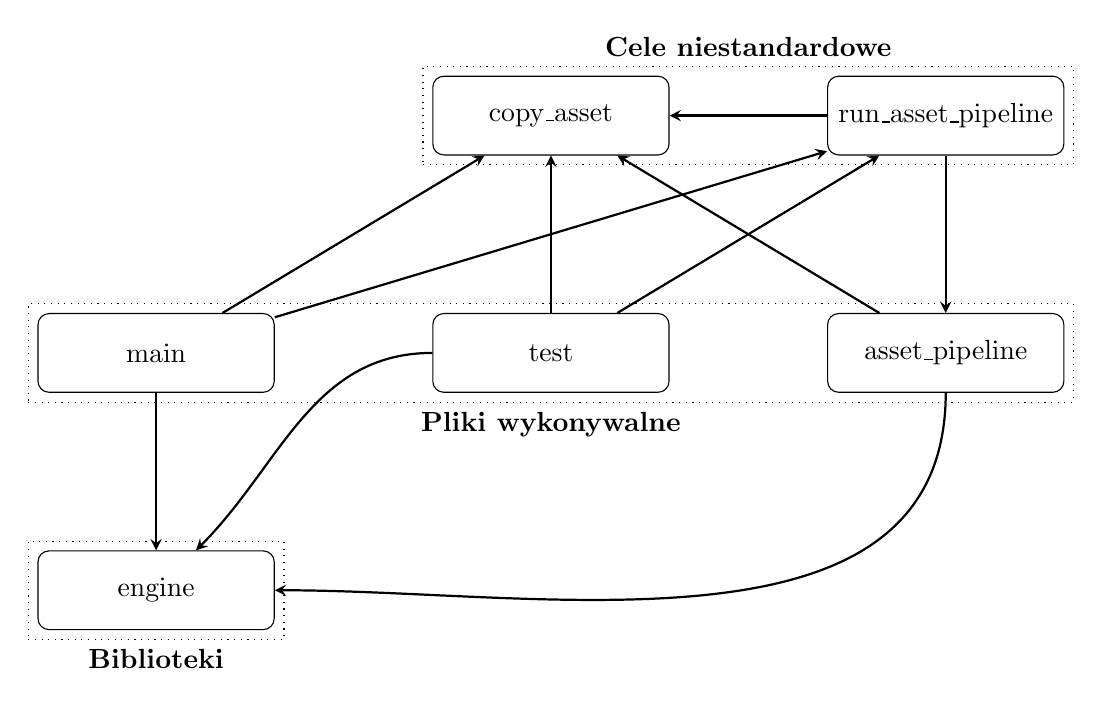
\begin{tikzpicture}[node distance=2cm]
		\tikzstyle{module} = [rectangle, rounded corners, minimum width=3cm, minimum height=1cm,text centered, draw=black]
		\tikzstyle{arrow} = [thick,->,>=stealth]
		
		\node (main) [module] {main};
		\node (test) [module, right = of main] {test};
		\node (assetpipeline) [module, right = of test] {asset\_pipeline};
		
		\node (engine) [module, below = of main] {engine};
		
		\node (runassetpipeline) [module, above = of assetpipeline] {run\_asset\_pipeline};
		\node (copyasset) [module, left = of runassetpipeline] {copy\_asset};
		
		\draw [arrow] (main) -- (engine);
		\draw [arrow] (test) edge[out=180, in=45] (engine);
		\draw [arrow] (assetpipeline) edge[out=-90, in=0] (engine);
		
		\draw [arrow] (main) edge[]  (runassetpipeline);
		\draw [arrow] (test) edge[]  (runassetpipeline);
		
		\draw [arrow] (runassetpipeline) -- (assetpipeline);
		
		\draw [arrow] (main) -- (copyasset);
		\draw [arrow] (test) -- (copyasset);
		\draw [arrow] (assetpipeline) -- (copyasset);
		\draw [arrow] (runassetpipeline) -- (copyasset);
		
		\node(plikiwykonywalne)[draw,dotted,fit=(main) (test) (assetpipeline)] {};
		\node (plikiwykonywalneLabel)[below=0cm of plikiwykonywalne] {\textbf{Pliki wykonywalne}};
		
		\node(biblioteki)[draw,dotted,fit=(engine)] {};
		\node (bibliotekiLabel)[below=0cm of biblioteki] {\textbf{Biblioteki}};
		
		\node(celeniestandardowe)[draw,dotted,fit=(copyasset) (runassetpipeline)] {};
		\node (celeniestandardoweLabel)[above=0cm of celeniestandardowe] {\textbf{Cele niestandardowe}};
		
	\end{tikzpicture}
	\caption{Proces budowania w formie celów i ich zależności (opracowanie własne)}
	\label{cmake}
\end{figure}

\paragraph{engine} Cel budujący bibliotekę programistyczną zawierającą implementację silnika.

\paragraph{main} Cel budujący plik wykonywalny demonstujący użycie silnika poprzez wyrenderowanie przykładowej sceny.

\paragraph{test} Cel budujący plik wykonywalny z testami jednostkowymi napisanymi i używanymi podczas implementowania projektu.

\paragraph{asset\_pipeline} Cel budujący plik wykonywalny służący jako narzędzie wiersza poleceń wykonujące operacje potoku zasobów.

\paragraph{copy\_assets} Niestandardowy cel kopiujący podkatalogu głównego \textit{assets} zawierającego nieprzetworzone zasoby wejściowe do katalogu budowania.

\paragraph{run\_asset\_pipeline} Niestandardowy cel realizujący potoku zasobów poprzez uruchomienie skryptu Python wielokrotne uruchamiającego narzędzie \textbf{asset\_pipeline} na zasobach wejściowych.


\subsection{Biblioteki zewnętrzne}

Projekt używa następujących zewnętrznych bibliotek programistycznych:

\begin{itemize}
	\item {\textit{Vulkan SDK 1.3.211.0}} \cite{VULKANSDK}:
	\begin{itemize}
		\item pliki nagłówkowe dla Vulkan,
		\item \textit{shaderc}: kompilacja shaderów z kodu źródłowego GLSL do kodu bajtowego SPIR,
		\item \textit{SPIRV-Reflect}: mechanizm refleksji dla kodu bajtowego SPIR-V,
	\end{itemize}
	\item {\textit{glfw 3.4}} \cite{GLFW}: wieloplatformowa obsługa tworzenia okien, obsługa wejścia klawiatury i myszy,
	\item {\textit{sqlite 3.35.5}} \cite{SQLITE}: relacyjna baza danych SQL,
	\item {\textit{uthash 2.3.0}} \cite{UTHASH}: proste struktury danych (tablica dynamiczna, lista dwukierunkowa, tablica mieszająca),
	\item {\textit{xxHash 0.8.1}} \cite{XXHASH}: niekryptograficzny algorytm mieszający,
	\item {\textit{cgltf 1.11}} \cite{CGLTF}: wczytywanie plików w formacie glTF,
	\item {\textit{cglm 0.8.5}} \cite{CGLM}: biblioteka matematyczna,
	\item {\textit{stb\_image 2.27}} \cite{STB}: wczytywanie obrazów,
	\item {\textit{stb\_truetype 1.26}} \cite{STB}: rasteryzacja tekstu czcionek,
	\item {biblioteka standardowa języka C} \cite{C11REFERENCE},
	\item {API systemu operacyjnego}: pliki nagłówkowe POSIX \cite{POSIXREFERENCE} albo WinAPI \cite{WINAPIREFERENCE},
	\item {biblioteka standardowa języka Python \cite{PYTHONREFERENCE}},
	\item {\textit{libclang 12.0.0}} \cite{LIBCLANG}: analizowanie kodu C w skryptach Python.
\end{itemize}

Dodatkowo biblioteka zbudowana w konfiguracji \textit{Debug} statycznie linkuje biblioteki \textit{ASan} (AddressSanitizer) i \textit{UBSan} (
UndefinedBehaviorSanitizer) wykrywające szeroką klasę błędów dotyczących niewłaściwego użycia pamięci i niezdefiniowanych zachowań. Błędy te w języku C są nieoczywiste i trudne do wykrycia przez programistę. Podczas rozwoju projektu ASan wielokrotnie pozwolił na wykrycie i naprawienie następujących rodzajów błędów:

\begin{itemize}
	\item wycieki pamięci,
	\item dereferencje zwisających wskaźników,
	\item dereferencja wskaźników NULL,
	\item dereferencja źle wyrównanych struktur,
	\item odczyt i zapis poza granicami tablicy.
\end{itemize}

\section{Architektura}

Silnik jest zaprojektowany w duchu architektury modułowej - funkcjonalność biblioteki jest rozdzielona na bloki zwane modułami, które mogą być rozwijane niezależnie od pozostałych modułów.

Obecne silnik składa się z następujących modułów:
\begin{itemize}
	\item Wygenerowany kod: mechanizmy metaprogramowania;
	\item Rdzeń: funkcje pomocnicze;
	\item I/O: wczytywanie bazy zasobów i konfiguracji;
	\item Zasoby: serializacja i deserializacja danych sceny z bazy zasobów;
	\item Vulkan: obsługa API Vulkan;
	\item Scena: operacje na grafie sceny;
	\item Renderer: graf renderowania i główna pętla programu.
\end{itemize}
Dodatkowo budowany jest plik wykonywalny demonstujący użycie silnika do wyrenderowanie przykładowej sceny używając grafu renderowania odroczonego.

Silnik był rozwijany metodą \textit{bottom-up} - jego pierwsza iteracja była pojedynczym plikiem źródłowym wyświetlającym trójkąt \cite{VULKANTUTORIAL}, który w procesie dekompozycji i refaktoryzacji organicznie rozrósł się do 7 modułów znajdujących się w osobnych podkatalogach zawierających łącznie 9 skryptów Python \textit{.py}, 65 nagłówków \textit{*.h} i 63 plików źródłowych \textit{*.c}.

Moduł jest dalej podzielony na jednostki, które zostały na potrzeby projektu zdefiniowane jako para składająca się z pliku nagłówkowego z odpowiadającym plikiem źródłowymi o tej samej nazwie.

Pliki nagłówkowe zawierają deklaracje funkcji, struktur oraz typów wyliczeniowych widocznych dla użytkownika końcowego i powinny być dołączone do programu przy użyciu dyrektywy \textit{\#include} preprocesora.
Pliki źródłowe zawierają definicje deklaracji plika nagłówkowego i powinny być dołączone do programu używając argumentów kompilatora (jeśli dodawane są niezbudowane pliki źródłowe) bądź linkera (jeśli dodawane są zbudowane pliki biblioteczne), co jest automatycznie wykonywane przez CMake.

Struktury są zorganizowane w sposób obiektowy.
Język C nie posiada wbudowanej koncepcji klasy, ale w projekcie przyjęto założenie, że dla klasy \textit{struct} jej stan jest reprezentowany przez strukturę \textit{struct}, która może posiadać metodę \textit{func()}, jeśli istnieje funkcja \textit{struct\_func()} przyjmująca wskaźnik do \textit{struct} jako pierwszy argument.
Dla obiektów globalnych nie jest istnieje osobna struktura przekazywana do jej metod - stan obiektu jest zaszyty w zmiennych globalnych jednostki translacji pliku źródłowego.

Obiekty mogą oferować metody \textit{create()} i \textit{destroy()}, które alokują lub dealokują instancję obiektu oraz tworzą bądź niszczą jej wewnętrzny stan.
Analogiczne metody \textit{init()} i \textit{deinit()} tworzą i niszczą instancję, której pamięć została wcześniej zaalokowaną (np. na stosie lub w tablicy).
Opcjonalna metoda \textit{debug\_print()} loguje informacje o wewnętrznym stanie instancji użyteczne podczas debugowania.

Diagram \ref{archit} przedstawia moduły silnika i ich najważniejsze jednostki.

\begin{figure}[H]
	\centering
	\begin{tikzpicture}[node distance=2mm]
		\tikzstyle{class} = [rectangle, minimum width=2cm, minimum height=5mm,text centered, draw=black]
		\tikzstyle{file} = [rectangle, minimum width=2cm, minimum height=5mm,text centered, draw=gray]
		\tikzstyle{file2} = [file, minimum width=3cm]
		\tikzstyle{executable} = [rectangle, rounded corners, minimum width=1cm, minimum height=5mm,text centered, draw=gray]

		\tikzstyle{arrow} = [thick,->,>=stealth]
		\tikzstyle{relation} = [densely dotted]
		
		% codegen
		\node (descriptors) [file] {descriptors};
		\node (constants) [file, below = of descriptors] {constants};
		\node (globals) [file, below = of constants] {globals};
		\node (macros) [file, below = of globals] {macros};
		\node (meta) [file, below = of macros] {meta};
		\node(codegen)[draw,dotted,fit=(descriptors) (meta)] {};
		
		% core
		\node (alloc) [file, below = 1cm of codegen] {alloc};
		\node (junk) [file, below = of alloc] {junk};
		\node (log) [file, below = of junk] {log};
		\node (platform) [file, below = of log] {platform};
		\node (thirdparty) [file, below = of platform] {thirdparty};
		\node(core)[draw,dotted,fit=(alloc) (junk) (log) (platform) (thirdparty)] {};
		
		% data
		\node (db) [file, below = 1cm of core] {sql\_db};
		\node (config) [file, below = of db] {config};
		\node (assetdb) [file, below = of config] {asset\_db};
		\node(data)[draw,dotted,fit=(db) (assetdb)] {};
		
		% assets
		\node (assetcommon) [file2, right = 2cm of platform] {asset\_common}; \def\y{assetcommon};
		\def\x{asset_camera}; \node (\x) [file2, below = of \y] {\myesc{\x}}; \edef\y{\x};
		\def\x{asset_direct_light}; \node (\x) [file2, below = of \y] {\myesc{\x}}; \edef\y{\x};
		\def\x{asset_material}; \node (\x) [file2, below = of \y] {\myesc{\x}}; \edef\y{\x};
		\def\x{asset_vertex_attribute}; \node (\x) [file2, right = of assetcommon] {\myesc{\x}}; \edef\y{\x};
		\def\x{asset_primitive}; \node (\x) [file2, below = of \y] {\myesc{\x}}; \edef\y{\x};
		\def\x{asset_mesh}; \node (\x) [file2, below = of \y] {\myesc{\x}}; \edef\y{\x};
		\def\x{asset_object}; \node (\x) [file2, below = of \y] {\myesc{\x}}; \edef\y{\x};
		\def\x{asset_image}; \node (\x) [file2, right = of asset_vertex_attribute] {\myesc{\x}}; \edef\y{\x};
		\def\x{asset_sampler}; \node (\x) [file2, below = of \y] {\myesc{\x}}; \edef\y{\x};
		\def\x{asset_texture}; \node (\x) [file2, below = of \y] {\myesc{\x}}; \edef\y{\x};
		\def\x{asset_skybox}; \node (\x) [file2, below = of \y] {\myesc{\x}}; \edef\y{\x};
		\def\x{asset_font}; \node (\x) [file2, below = of \y] {\myesc{\x}}; \edef\y{\x};
		\node (assetpipeline) [executable, below = of asset_object] {asset\_pipeline};
		\node(assets)[draw,dotted,fit=(assetcommon) (asset_font)] {};
	
		% scene
		\node (scene_data) [file, right = 3.6cm of junk] {scene\_data}; \def\y{scene_data};
		\def\x{scene_graph}; \node (\x) [file, right = of \y] {\myesc{\x}}; \edef\y{\x};
		\def\x{scene_tree}; \node (\x) [file, right = of \y] {\myesc{\x}}; \edef\y{\x};
		\node(scene)[draw,dotted,fit=(scene_data) (scene_tree)] {};
		
		% vulkan
		\node (buffer) [file, right = 1.5cm of descriptors] {buffer}; \def\y{buffer};
		\def\x{image}; \node (\x) [file, below = of \y] {\myesc{\x}}; \edef\y{\x};
		\def\x{vertex_stream};\node (\x) [file, below = of \y] {\myesc{\x}}; \edef\y{\x};
		\def\x{device}; \node (\x) [file, right = 1cm of buffer] {\myesc{\x}}; \edef\y{\x};
		\def\x{swap_chain}; \node (\x) [file, below = of \y] {\myesc{\x}}; \edef\y{\x};
		\def\x{sync}; \node (\x) [file, below = of \y] {\myesc{\x}}; \edef\y{\x};
		\def\x{unified_constant_buffer}; \node (\x) [file, below = 4mm of vertex_stream] {\myesc{\x}}; \edef\y{\x};
		\def\x{textures}; \node (\x) [file, below = of \y] {\myesc{\x}}; \edef\y{\x};
		\def\x{unified_geometry_buffer}; \node (\x) [file, below = of \y] {\myesc{\x}}; \edef\y{\x};
		\def\x{descriptor};\node (\x) [file, right = 1mm of unified_constant_buffer] {\myesc{\x}}; \edef\y{\x};
		\def\x{shader};\node (\x) [file, below = of \y] {\myesc{\x}}; \edef\y{\x};
		\node(objects)[draw,dotted,fit=(device) (unified_geometry_buffer) (shader)] {};
		
		% renderer
		\node (renderer) [file, right = 7mm of device] {renderer}; \def\y{renderer};
		\def\x{render_state}; \node (\x) [file, below = of \y] {\myesc{\x}}; \edef\y{\x};
		\def\x{renderer_cache}; \node (\x) [file, below = of \y] {\myesc{\x}}; \edef\y{\x};
		\def\x{render_graph}; \node (\x) [file, right = of render_state] {\myesc{\x}}; \edef\y{\x};
		\def\x{render_pass}; \node (\x) [file, below = of \y] {\myesc{\x}}; \edef\y{\x};
		\def\x{render_pass_state}; \node (\x) [file, below = of \y] {\myesc{\x}}; \edef\y{\x};
		\def\x{batch}; \node (\x) [file, left = of render_pass_state] {\myesc{\x}}; \edef\y{\x};
		\def\x{main}; \node (\x) [executable, right = 0.7cm of renderer] {\myesc{\x}}; \edef\y{\x};
		\node(rendering)[draw,dotted,fit=(renderer) (renderer_cache) (render_pass_state) (main) (batch)] {};
	
		% labels
		\node ()[above=0cm of codegen] {\textbf{Wygenerowany kod}};
		\node ()[above=0cm of core] {\textbf{Rdzeń}};
		\node ()[above=0cm of data] {\textbf{I/O}};
		\node ()[below=0cm of assets] {\textbf{Zasoby}};
		\node ()[above=0cm of objects] {\textbf{Vulkan}};
		\node ()[below=0cm of scene] {\textbf{Scena}};
		\node ()[above=0cm of rendering] {\textbf{Renderer}};
		
	\end{tikzpicture}
	\caption{Relacje pomiędzy modułam silnika i ich najważniejszymi klasami (opracowanie własne)}
	\label{archit}
\end{figure}

\section {Implementacja}

Ta sekcja opisuje szczegóły implementacyjne poszczególnych modułów silnika.

\subsection{Wygenerowany kod}

Silnik używa kodu w języku C wygenerowanego przez automatyczny generator kodu będący skryptem Python uruchamianym przez CMake na początku procesu budowania przed rozpoczęciem kompilacji właściwego
kodu źródłowego biblioteki.

Język C nie posiada mechanizmów pozwalających na metaprogramowanie z wyjątkiem makr preprocesora, które mogą zaspokoić część potrzeb programisty chcącego przykładowo dodać nowy rodzaje pętli \cite{METACONTROLC}, ale nie pozwalają na bardziej skomplikowaną analizę i przekształcanie kodu, które muszą być wykonywane przez zewnętrzne narzędzia.

Działanie skryptu jest sterowane konfiguracją generatora, który jest plikiem w formacie INI (zgodnym z biblioteką \textit{configparser} \cite{PYTHONCONFIGPARSER}) znajdującym się w katalogu ze skryptem.
Format INI nie posiada standardowej specyfikacji, ale tradycyjnie jest on plikiem tekstowym podzielonym na sekcje zawierające pary klucz-wartość.

Skrypt parsuje pliki nagłówkowe języka C znajdujący się w katalogu /src z
pominięciem katalogu /src/codegen, do którego skrypt zapisuje wygenerowane pliki nagłówkowe i źródłowe, które są kolejno dołączane w innych modułach silnika i dodawane jako argumenty kompilatora.
Razem wszystkie wygenerowane pliki tworzą jednostki modułu wygenerowanego kodu.


\subsubsection{Jednostka constants}
Zawiera wygenerowane stałe: wartości zdefiniowane w sekcji \textit{CONSTANTS} konfiguracji generatora używane przez resztę modułów, które zostały uznane za zbyt niepraktyczne aby pozwolić na ich modyfikację przy użyciu konfiguracji globalnej.
Poniżej wymieniono stałe, ich wartości oraz interpretacje:
\begin{itemize}
	\item \textit{FRAMES\_IN\_FLIGHT}: $2$, liczba klatek w locie (ang. in flight frames), czyli jednocześnie renderowanych przez GPU, domyślna wartość pozwala na podwójne buforowanie; 
	\item \textit{MAX\_OFFSCREEN\_TEXTURE\_COUNT}: $16$, maksymalna liczbę tekstur pozaekranowych;
	\item \textit{MAX\_RENDER\_TARGET\_COUNT}: $8$, maksymalną liczbę tekstur pozaekranowych, które mogą być używane jako cele renderowania podczas jednego przebiegu; 
	\item \textit{MAX\_FRAMEBUFFER\_ATTACHMENT\_COUNT}: \textit{MAX\_RENDER\_TARGET\_COUNT + 1 + 1}, maksymalna liczba dołączeń używana przez potok graficzny - wystarcza na dołączenia celów renderowania, prezentowalnego obrazu i bufor głębi;
	\item \textit{MAX\_INDIRECT\_DRAW\_COMMAND\_COUNT}: $1024$, maksymalna liczba poleceń rysowania które mogą być wykonana przez jedno polecenie rysowania pośredniego;
	\item \textit{MAX\_MATERIAL\_COUNT}: $128$, maksymalna liczba materiałów;
	\item \textit{MAX\_DIRECTIONAL\_LIGHT\_COUNT}: $1$, maksymalna liczbę świateł kierunkowych na scenie;
	\item \textit{MAX\_POINT\_LIGHT\_COUNT}: $128$, maksymalna liczbę świateł punktowych na scenie;
	\item \textit{MAX\_TEXT\_CHARACTER\_COUNT}: $256$, maksymalną liczbę znaków w renderowanym ciągu znaków;
	\item \textit{MIN\_DELTA\_TIME}: $(1.0 / 30.0)$, minimalny czas pomiędzy wywołaniami funkcji zwrotnej \textit{update} w pętli głównej, domyślnie $\frac{1}{30}$ sekundy (30 FPS);
	\item \textit{WORLD\_UP}: $0, 1, 0$; wektor interpretowany jako "w górę" w przestrzeni świata.
\end{itemize}

Wygenerowane stałe mogą być używane przez shadery - ich definicje są umieszczane na początku kodu GLSL shadera przed jego kompilacją - dlatego są one udostępniane w formie X-makro \textit{CODEGEN\_CONSTANTS}.

X-makro to przydatna technika preprocesora pozwalająca na pisanie kodu, który jest automatycznie aktualizowany po zmianie danych opisywanych przez X-makro \cite{XMACRO}.
Przykładowo funkcja przedstawiona na listingu \ref{xmacroBefore} wymaga manualnej aktualizacji po zmianie używanego typu wyliczeniowego.
\lstset{language=C}
\begin{lstlisting}[caption={Przykładowy kod przed zastosowaniem X-makro},captionpos=b,label={xmacroBefore}]
typedef enum key {
	key_space,
	key_enter,
	key_count,
} key;

int key_to_glfw_key(key value) {
	switch (value) {
		case key_space: return GLFW_KEY_SPACE;
		case key_enter: return GLFW_KEY_ENTER;
		default: return GLFW_KEY_UNKNOWN;
	}
}
\end{lstlisting}
Listing \ref{xmacroAfter} przedstawia użycie X-makro do przepisania kodu z listingu \ref{xmacroBefore}:
\lstset{language=C}
\begin{lstlisting}[caption={Przykładowy kod po zastosowaniu X-makro},captionpos=b,label={xmacroAfter}]

#define END_OF_KEYS
#define KEYS(X, ...)			\
	X(space, GLFW_KEY_SPACE)	\
	X(enter, GLFW_KEY_ENTER)	\
	END_OF_KEYS

typedef enum key {
#define x(_name, ...) key_##_name,
	KEYS(x, )
#undef x
	key_count,
} key;

int key_to_glfw_key(key value) {
	switch (value) {
#define x(_name, _value, ...) case key_##_name: return _value;
		KEYS(x, )
#undef x
		default: return GLFW_KEY_UNKNOWN;
	}
}
\end{lstlisting}


\subsubsection{Jednostka globals}
Obiekt globalny \textit{globals} reprezentujący wygenerowane zmienne.
Ich wartości, w przeciwieństwie do stałych, mogą być ustalone dopiero w czasie wykonywania.
Obiekt jest używany do specyfikacji struktury różnych ścieżek katalogów i plików używanych przez silnik.

Listing \ref{configGenBefore} przedstawią sekcję konfiguracji generacji opisującą ścieżki dla katalogu zasobów, konfiguracji globalnej, bazy zasobów, katalogu shaderów i ich współdzielonego kodu GLSL oraz pliku logowania.
\lstset{language=verbatim}
\begin{lstlisting}[caption={Konfiguracja generacji zmiennych},captionpos=b,label={configGenBefore}]
[GLOBALS]
assetsDirname = assets
assetDatabaseFilepath = ${assetsDirname}/data.db
assetConfigFilepath = ${assetsDirname}/config.ini
assetsShaderDirpath = ${assetsDirname}/shaders
assetsShaderCommonFilepath = ${assetsShaderDirpath}/common.glsl
logFileName = log.txt
\end{lstlisting}
Listing \ref{configGenAfter} przedstawia wygenerowaną metodę \textit{init()}.
\lstset{language=C}
\begin{lstlisting}[caption={Wynik generacji zmiennych},captionpos=b,label={configGenAfter}]
void globals_create() {
	globals.assetsDirname =
		get_executable_dir_file_path("", "assets");
	globals.assetDatabaseFilepath =
		get_executable_dir_file_path("", "assets/data.db");
	globals.assetConfigFilepath =
		get_executable_dir_file_path("", "assets/config.ini");
	globals.assetsShaderDirpath =
		get_executable_dir_file_path("", "assets/shaders");
	globals.assetsShaderCommonFilepath =
  		get_executable_dir_file_path("", "assets/shaders/common.glsl");
	globals.logFileName =
		get_executable_dir_file_path("", "log.txt");
}
\end{lstlisting}

\subsubsection{Jednostka macros}
Zbiór X-makr używanych przez moduł I/O obsługujący następujące zasoby wejściowe.

Makra opisują wewnętrzną strukturę plików INI konfiguracji globalnej i konfiguracji zasobów: używane sekcje i ich dopuszczalne pary klucz-wartość z domyślnymi wartościami (liczby całkowite bądź ciągi znaków).
Listing \ref{macrosBefore} przedstawia przykładowy fragment konfiguracji generatora opisujący konfigurację globalną i pozwalający na sparsowanie pliku INI przedstawionego na listingu \ref{macrosAfter}.
\lstset{language=verbatim}
\begin{lstlisting}[caption={Konfiguracja generacji konfiguracji globalnej},captionpos=b,label={macrosBefore}]
[GLOBAL.CONFIG]
graphics.WindowWidth = 640
controls.Enabled = 1
settings.StartScene = "sponza"
\end{lstlisting}

\lstset{language=verbatim}
\begin{lstlisting}[caption={Przykładowa konfiguracja globalna},captionpos=b,label={macrosAfter}]
[settings]
StartScene = MetalRoughSpheresNoTextures

[graphics]
WindowWidth = 1024

[controls]
Enabled = 1 
\end{lstlisting}

Podobnie opisywana jest struktura bazy zasobów: typy podstawowe i ich odpowiedniki w języku C oraz tabele i ich kolumny. Ilustruje to fragment konfiguracji generatora przedstawiony na listingu \ref{macrosDB}.
\lstset{language=verbatim}
\begin{lstlisting}[caption={Fragment konfiguracji generatora opisujący strukturę bazy zasobów},captionpos=b,label={macrosDB}]
[ASSET.DB]
types = "BYTE:uint8_t, INT:uint32_t, FLOAT:float, TEXT:UT_string *, KEY:hash_t"
image = "key KEY, width INT, height INT, depth INT, channels INT, type INT, data BYTE_ARRAY"
sampler = "key KEY, magFilter INT, minFilter INT, addressWrapU INT, addressWrapV INT"
texture = "key KEY, image KEY, sampler KEY"
\end{lstlisting}

Struktura zasobów wejściowych zostanie dokładniej opisana w dalszym podrozdziale o module I/O.

\subsubsection{Jednostka meta}
Funkcje pomocnicze wygenerowane na podstawie nagłówków silnika i Vulkan SDK.

Dla każdego napotkanego typu wyliczeniowego \textit{EnumName} jest generowana jedna z funkcji, których prototypy zostały przedstawione na listingu \ref{metaProtos}.
\lstset{language=C}
\begin{lstlisting}[caption={Wygenerowane funkcje dla typów wyliczeniowych},captionpos=b,label={metaProtos}]
const char *EnumName_debug_str(int value);
void EnumName_debug_print(int flags, int indent);
\end{lstlisting}
Funkcje pozwalające na konwersję liczby całkowitej będącej wartoścą zmiennej wyliczeniowego na ciąg znaków i są używane przez metody \textit{debug\_print()} do logowania wartości w formie przyjaźniejszej dla użytkownika.

Funkcja \textit{*\_debug\_str()} jest generowana tylko wtedy, jeśli literały wyliczeniowe nie są flagami, tj. nie są kolejnymi potęgami liczby 2.


\subsubsection{Jednostka descriptors}
Jednostka zawierająca struktury i funkcje upraszczające pracę z deskryptorami.

Nagłówek \textit{descriptor} modułu Vulkan zawiera definicje struktur języka C opisujących wewnętrzną strukturę pamięci buforów i stałych push znajdujących się na GPU.
W zależności od nazwy dzielą się one na 3 rodziny:
\begin{itemize}
	\item \textit{*\_push\_constant\_struct}: stała push o nazwie \textit{*},
	\item \textit{*\_uniform\_buffer\_struct}: bufor uniform o nazwie \textit{*},
	\item \textit{*\_helper\_struct}: struktura pomocnicza o nazwie \textit{*} używana w powyższych.
\end{itemize}
Listing \ref{descriptorsBefore} przedstawia przykłady powyższych struktur.
\lstset{language=C}
\begin{lstlisting}[caption={Przykładowe struktury w nagłówku descriptor opisujące wewnętrzną strukturę deskryptorów},captionpos=b,label={descriptorsBefore}]
// stała push 'draw'
typedef struct draw_push_constant_struct {
	uint currentFrameInFlight;
} draw_push_constant_struct;

// struktura pomocnicza 'offscreen_texture'
typedef struct offscreen_texture_helper_struct {
	uint textureId; ///< array=MAX_OFFSCREEN_TEXTURE_COUNT
} offscreen_texture_helper_struct;

// stała push 'global'
typedef struct global_uniform_buffer_struct {
	mat4 viewMat;
	mat4 projMat;
	...
	offscreen_texture_helper_struct offscreenTextures;
} global_uniform_buffer_struct;
\end{lstlisting}

Układ pamięci struktur zdefiniowanych w języku C nie jest koniecznie kompatybilny z układem pamięci wymaganym przez GPU.
Dlatego dla każdej sparsowanej struktury \textit{*\_struct} jest generowana analogiczna struktura \textit{*\_element}, w których użyto specyfikatorów \textit{alignas} i atrybutów \textit{packed} udostępnianych przez C11 i rozszerzenia GCC w celu wyrównania pól struktury w zgodzie ze standardem układu pamięci scalar.
Generowana jest też funkcja \textit{glsl\_add\_*()} dodająca do ciągu znaków z kodem GLSL definicje struktury i kwalifikator układu.
Listing \ref{descriptorsAfter} pokazuje przykładowe wejście i wyjście generacji dla bufora uniform \textit{instances}.
\lstset{language=C}
\begin{lstlisting}[caption={Przykładowe wejście i wyjście generacji dla bufora uniform},captionpos=b,label={descriptorsAfter}]
// descriptor.h:
typedef struct instances_uniform_buffer_struct {
	mat4 modelMat;
	uint materialId;
} instances_uniform_buffer_struct;
	
// descriptors.h
typedef struct PACKED_STRUCT instances_uniform_buffer_element {
	alignas(4) mat4 modelMat ;
	alignas(4) uint materialId ;
} instances_uniform_buffer_element;
void glsl_add_instances_uniform_buffer(
	UT_string *s, uint32_t set, uint32_t binding, uint32_t count);

// descriptors.c
void glsl_add_instances_uniform_buffer(
	UT_string *s, uint32_t set, uint32_t binding, uint32_t count) {
	utstring_printf(s, "struct instancesStruct {\n");
	utstring_printf(s, "  mat4 modelMat ;\n");
	utstring_printf(s, "  uint materialId ;\n");
	utstring_printf(s, "};\n");
	utstring_printf(s, "layout(scalar, set = %u, binding = %u) "
			   "uniform instancesBlock {\n", set, binding);
	utstring_printf(s, "  instancesStruct instances");
	if (count > 1) {utstring_printf(s, "[%u]", count);}
	utstring_printf(s, ";\n};\n");
}
\end{lstlisting}
Generacja jest kończona X-makrami wyliczającymi nazwy wszystkich sparsowanych rodzin struktur. 

Dzięki automatycznej generacji kodu modyfikacja sposobu organizacji pamięci GPU buforów sprowadza się do modyfikacji struktur w nagłówku \textit{descriptors}, co pozwala na szybkie testowanie nowych parametrów i metod dostępu do nich podczas pisania shaderów.
Mechanizm ten został zainspirowany implementacją jednolitych buforów w grze \textit{Tom Clancy's Rainbow Six Siege} \cite{RAINBOWSIXSIEGE}.

Wygenerowane struktury, funkcje i X-makra są używane podczas kopiowania danych z CPU do pamięci GPU oraz generacji shaderów, co zostanie dokładniej opisane w dalszym podrozdziale o module Vulkan.

\subsection{Rdzeń}

Rdzeń to moduł zawierający funkcje pomocniczych i obiekty globalne zapewniające podstawowe funkcjonalności używane przez resztę modułów.

\subsubsection{Jednostka thirdparty}
Jednostka odpowiedzialna za udostępnienia bibliotek zewnętrznych reszcie kodu.

Nagłówek dołącza nagłówki bibliotek zewnętrznych i z powodów wydajnościowych podczas procesu budowania jest traktowany jako nagłówek prekompilowany (ang. precompiled header, PCH).

Plik źródłowy obsługuje część bibliotek zewnętrznych składających się jedynie z nagłówków (ang. header-only library).
W przeciwieństwie do tradycyjnych bibliotek języka C w których kod jest podzielony na pliki nagłówkowe i źródłowe, w tym przypadku dostęp do definicji tradycyjnie znajdujących się z plikach źródłowych jest uzyskiwany poprzez ponowne dołączenie nagłówka przy użyciu dyrektywy \textit{\#include} po wcześniejszym zdefiniowaniu odpowiedniego symbolu preprocesora.
Listing \ref{thirdpartyCgltf} przedstawia wymagany sposób ponownego dołączenia nagłówka biblioteki \textit{cgltf}.
\lstset{language=C}
\begin{lstlisting}[caption={Przykład dołączenia implementacji biblioteki \textit{cgltf}},captionpos=b,label={thirdpartyCgltf}]
#define CGLTF_IMPLEMENTATION
#include "cgltf.h"
\end{lstlisting}

\subsubsection{Jednostka alloc}
Funkcje pomocnicze wspomagające zarządzanie pamięcią CPU, co obejmuje alokację, dealokację, kopiowanie, duplikowanie i porównywanie bloków pamięci CPU.

Funkcje te są potrzebne, ponieważ działanie odpowiednich funkcji oferowane przez bibliotekę standardową języka C, chociaż oferują żądaną funkcjonalność, opiera się na mechanizmie niezdefiniowanych zachowań (ang. undefined behaviour) dla niektórych argumentów (wskaźnik NULL, rozmiar 0) i zachowań OOM (ang. out-of-memory, brak pamięci).

Funkcje pomocnicze są wrapperami z dodatkowymi instrukcjami warunkowymi sprawdzającymi, czy wywołanie funkcji nie skutkuje niezdefiniowanym zachowaniem.

Jednostka definiuje też makra ułatwiające zarządzanie pamięcią struktur danych biblioteki \textit{uthash}.


\subsubsection{Jednostka log}
Obiekt globalny \textit{log} reprezentujący system logowana komunikatów wygenerowanych podczas działania kodu mający na celu w uproszczenie procesu debugowania.

Komunikat jest ciągiem znaków z przypisanym poziomem logowania określającym jego ważność z domyślnie wspieranymi wartościami \textit{debug}, \textit{info}, \textit{warn}, \textit{error} i \textit{fatal}.
Komunikaty \textit{debug} są logowane tylko w konfiguracji \textit{Debug}.

Komunikaty są zapisywane do standardowego wyjścia (\textit{stdout} albo \textit{stderr}) oraz do pliku tekstowego na dysku, którego nazwa została zdefiniowana w wygenerowanych zmiennych (domyślnie \textit{log.txt}).

Logowanie komunikatu odbywa się poprzez grupę funkcji \textit{log\_*()}, gdzie \textit{*} to poziom logowania, zachowujące się tak samo jak funkcja \textit{printf()} z biblioteki standardowej języka C - pierwszy argument to ciąg znaków z znakami formatującymi, reszta argumentów to formatowane wartości.

Listing \ref{logBefore} demonstruje logowanie i powinien zapisać do pliku \textit{log.txt} w katalogu z plikiem wykonywalnym komunikaty podobne do przedstawionych na listingu \ref{logAfter}:
\lstset{language=C}
\begin{lstlisting}[caption={Demonstracja logowania},captionpos=b,label={logBefore}]
log_create();
log_debug("komunikat #%d", 1);
log_debug("komunikat #%d", 2);
log_fatal("%s #%d", "komunikat", 3);
log_destroy();
\end{lstlisting}

\lstset{language=verbatim}
\begin{lstlisting}[caption={Wynik logowania},captionpos=b,label={logAfter}]
[DEBUG] (/home/user/repo/src/main.c:45) main:
komunikat #1
komunikat #2
[FATAL] (/home/user/repo/src/main.c:47) main:
komunikat #3
\end{lstlisting}

\subsubsection{Jednostka junk}
Proste funkcje i makra które mogą być potencjalnie używane we wszystkich modułach biblioteki, ale nie zostały uznane za wystarczająca skomplikowane, aby uzasadnić wydzielenia do osobnej jednostki.

Jednostka definiuje stałe preprocesora \textit{PLATFORM\_*} przedstawione na listingu \ref{junk1} używane do rozpoznania systemu operacyjnego, na którym budowany jest silnik (Linux, MacOS, Windows).
\lstset{language=C}
\begin{lstlisting}[caption={Stałe preprocesora używane do rozpoznania systemu operacyjnego},captionpos=b,label={junk1}]
#if defined(__linux) || defined(__linux__) || defined(linux)
#define PLATFORM_LINUX
#elif defined(__APPLE__)
#define PLATFORM_APPLE
#elif defined(_WIN32) || defined(__WIN32__) \
   || defined(WIN32) || defined(_WIN64)
#define PLATFORM_WINDOWS
#endif
\end{lstlisting}

Funkcja \textit{strstrip()} usuwa początkowe i końcowe białe znaki z ciągu znaków.

Funkcja \textit{count\_bits()} zlicza bity w liczbie całkowitej używając metody Briana Kernighana \cite{BITTWIDDLINGHACKS}. Przykładem użycia jest określenie liczby flag ustawionych w wyliczeniu.

Makra \textit{HASH\_*} ukrywają detale użycie funkcji skrótu biblioteki \textit{xxHash} i zostały przedstawione na listingu \ref{junk2}.
\lstset{language=C}
\begin{lstlisting}[caption={Przykład użycia funkcji skrótu},captionpos=b,label={junk2}]
hash_t hash;
HASH_START(hashState)
HASH_UPDATE(hashState, &num, sizeof(num))
HASH_UPDATE(hashState, str, strlen(str))
HASH_UPDATE(hashState, &object->field, sizeof(object->field))
HASH_DIGEST(hashState, hash)
HASH_END(hashState)
log_debug("Hash value is %zu", hash);
\end{lstlisting}

Makro \textit{UNREACHABLE} pozwala na optymalizację kodu poprzez oznaczenie punktów programu, które nigdy nie są napotykane przez przepływ sterowania.
Jego definicja zależy od konfiguracji: w \textit{Debug} sprowadza się do asercji \textit{assert(0)}, a w \textit{Release} do funkcji wbudowanej kompilatora GCC \textit{\_\_builtin\_unreachable()}.
Przykładowo określenie nieosiągalności przypadku domyślnej instrukcji switch bądź bloku else informuje o
kompletności sprawdzanych warunków, co zostało przedstawione na listingu \ref{junk3}.
\lstset{language=C}
\begin{lstlisting}[caption={Przykład użycia makra UNREACHABLE},captionpos=b,label={junk3}]
if (type == directional) {
	...
} else if (type == point) {
	...
} else {
	UNREACHABLE;
}
\end{lstlisting}

Jednostka definiuje też makra używające formy metaprogramowania w celu dodania nowych struktur kontrolnych \cite{METACONTROLC} upraszczających iterowanie po strukturach danych biblioteki \textit{uthash}, której użycie zostało przedstawione na listingu \ref{junk4}.
\lstset{language=C}
\begin{lstlisting}[caption={Przykład iteracji używając makra utarray\_foreach\_elem\_deref},captionpos=b,label={junk4}]
utarray_foreach_elem_deref (tree_node *, node, tree->nodes) {
	tree_set_dirty(tree, node);
}
\end{lstlisting}


\subsubsection{Jednostka platform}
Głowna część rdzenia implementująca obiekt globalny \textit{platform} odpowiedzialny za tworzenie i niszczenie globalnego stanu używanego przez system logowania i funkcje wieloplatformowe, z których najważniejsze zostały opisane poniżej.

Funkcja \textit{panic()} pozwala na zamknięcie programu z kodem wyjścia oznaczającym nieudane wykonanie po wystąpieniu fatalnego błędu.
Jest ona używana przez makro \textit{verify()}, które podobnie do makra \textit{assert()} pozwala na testowanie warunku logicznego i przerwanie działania programu gdy przyjmuje on wartość fałsz, ale w przeciwieństwie do niego działa też w konfiguracji \textit{Release}.

Funkcje \textit{get\_executable\_dir\_path()} i \textit{get\_path\_dirname()} pozwalają na odkrycie ścieżki z katalogiem zawierającym plik wykonywalny, co jest potrzebne do pełnego określenia struktury plików opisanych przez wygenerowane stałe.
Na systemie Linux używana jest funkcja \textit{readlink()} do odczytania pliku \textit{/proc/self/exe}
oraz funkcja \textit{dirname()}.
Na systemie Windows używana jest funkcja \textit{GetModuleFileName()} oraz funkcja \textit{PathRemoveFileSpec()}.

Funkcje \textit{write\_text\_file()} i \textit{read\_text\_file()} pozwalają na odczyt i zapis plików tekstowych i są używane do obsługi konfiguracji i kodu źródłowego shaderów.

\subsection{I/O}

Silnik wczytuje ze ścieżek zaszytych w zmiennych globalnych następujące zasoby wyjściowe:
\begin{itemize}
	\item konfiguracja globalna (plik tekstowy INI),
	\item kod GLSL shadera (plik tekstowy GLSL),
	\item baza zasobów (baza danych).
\end{itemize}

Wszystkie zasoby wejściowe które muszą być łatwo edytowalne przez użytkownika są plikami tekstowymi i są bezpośrednio kopiowane przez potok zasobów do katalogu budowania stając się zasobami wyjściowymi.
Reszta zasobów wejściowych staje się częścią bazy zasobów będącej plikiem bazy danych SQLite.

SQLite \cite{SQLITE} to biblioteka języka C implementująca silnik relacyjnej bazy danych SQL.
Jest ona bardzo popularnym wyborem jako format pliku używany do utrwalania stanu aplikacji na dysku z wielu powodów, do których zalicza się prosta użycia, wysoka wydajności, bogata wewnętrzna struktura oferowana przez relacyjną bazę danych i formę łatwego do dystrybucji pojedynczego samodzielnego pliku na dysku \cite{SQLITEAPPFORMAT}.

Moduł I/O zawiera obiekty używane do wczytywania i zapisywania powyższych zasobów wraz z walidacją ich formatu i wewnętrznej struktury - interpretacją danych zajmują się dalsze moduły.

\subsubsection{Jednostka config}
Obiekt \textit{data\_config} reprezentujący pojedynczy plik INI zawierający jeden z dwóch rodzajów konfiguracji: konfigurację globalną lub konfigurację zasobów.

\textbf{Konfiguracja globalna} jest ładowana na samym początku inicjalizacji silnika i pozwala użytkownikowi na sterowanie jego działania poprzez zmianę następujących zmiennych:
\begin{itemize}
	\item sekcja \textit{graphics}:
	\begin{itemize}
		\item \textit{WindowWidth}, \textit{WindowHeight}, \textit{WindowTitle}: szerokość, wysokość i tytuł okna,
		\item \textit{EnabledInstancing}: włączenie instancjonowania,
		\item \textit{MaxPrimitiveElementCount}: maksymalna liczba prymitywów renderowania,
		\item \textit{Font}: czcionka,
	\end{itemize}
	\item sekcja \textit{controls}:
	\begin{itemize}
		\item \textit{Enabled}: obsługa danych wejściowych myszy i klawiatury,
	\end{itemize}
	\item sekcja \textit{settings}:
	\begin{itemize}
		\item \textit{StartScene}: nazwa sceny ładowanej z bazy zasobów.
	\end{itemize}
\end{itemize}

\textbf{Konfiguracja zasobów} jest używana wyłącznie przez potok zasobów i zawiera dodatkowe informacje o przetwarzanym zasobie wejściowym takie jak:
\begin{itemize}
	\item sekcja \textit{skybox}:
	\begin{itemize}
		\item \textit{Name}: nazwa używanej tekstury skybox.
	\end{itemize}
\end{itemize}

Konfiguracja jest zbiorem par klucz-wartość.
Wartości mogą być liczbą całkowitą lub ciągiem znaków i dla brakujących klucze mają wartość domyślną.
Odczyt i zapis odbywa się przy pomocy metod \textit{load()} i \textit{save()}.


\subsubsection{Jednostka sql\_db}
Obiekt \textit{sql\_db} reprezentujący połączenie z plikiem bazy danych SQLite.

SQLite posiada dynamiczny i słaby system typowania posiadający 5 typów prostych:
NULL, INTEGER (liczba całkowita maksymalnie 64-bitowa), REAL (64-bitowa liczba zmiennoprzecinkowa), TEXT ( ciąg znaków UTF-8/16) i BLOB: (blok pamięci).
Obiekt \textit{db} rozszerza ten ubogi system typów nowymi typami złożonymi bezpośrednio odpowiadającymi typom języka C zdefiniowanych w konfiguracji generatora: BYTE (uint8\_t), INT (uint32\_t), FLOAT (float), VEC2(vec2), VEC3(vec3), VEC4(vec4), MAT4(mat4), TEXT(UT\_string *), i KEY(hash\_t).
Dodatkowo każdy typ posiada wersję tablicową \textit{*\_ARRAY} (BYTE\_ARRAY, INT\_ARRAY itd.).

Obiekt \textit{sql\_db} pozwala na przeprowadzanie standardowych operacji wyboru (ang. select) i umieszczania (ang. insert) rekordów do wybranej tabeli.
Baza danych SQLite wciąż wewnętrznie używa typów prostych, ale wygenerowane przy użyciu X-makro metody \textit{select\_*()} i \textit{insert\_*()} automatycznie przeprowadzają serializację i deserializację typów złożonych.


\subsubsection{Jednostka asset\_db}
Obiekt \textit{asset\_db} reprezentuje bazę zasobów.
Używa on wewnętrznie obiektu \textit{sql\_db} i podobnie jak w nim użyto X-makro do dodania metod wyboru i umieszczania wartości dla specyficznej tabeli, kolumny i klucza.

Listing \ref{assetDbExample} demonstruje wybór i umieszczenie kod wartość FLOAT z tabeli \textit{directLight}, kolumny \textit{intensity} i klucza \textit{key}.
\lstset{language=C}
\begin{lstlisting}[caption={Deserializacja i serializacja wartości zmiennoprzecinkowej},captionpos=b,label={assetDbExample}]
float value =
	asset_db_select_directLight_intensity_float(assetDb, key).value;
asset_db_insert_directLight_intensity_float(assetDb, key,
	data_float_temp(value));
\end{lstlisting}

Obiekt ten jest intensywnie używany przez moduł zasobów do implementacji serializacji i deserializacji.

\subsection{Zasoby}

Moduł zawierajacy obiekty zasobów, które pozwalają na serializację i deserializację indywidualnych zasobów z bazy zasobów do formy używalnej przez resztę kodu silnika.

Wszystkie obiekty zasobów mają nazwy w formie \textit{asset\_*} i współdzielą następujące pola i metody:
\begin{itemize}
	\item klucz zasobu: jednoznacznie identyfikuje obiekt jako unikalny zasób i jest otrzymywany poprzez użycie funkcji skrótu na jego polach.
	\item wskaźnik do obiektu \textit{scene\_data} z modułu sceny: obiekty zasobów są zarządzane przez wskazywany obiekt zawierający dane sceny. Może być on używany podczas deserializacji.
	\item wskaźniki \textit{prev} i \textit{next}: pozwalają na użycie obiektu w liście dwukierunkowej biblioteki \textit{uthash}.
	\item \textit{calculate\_key()}: oblicza klucz zasobu, musi być wywoływany po każdej modyfikacji obiektu.
	\item \textit{serialize()}: serializacja, czyli zapis pól do bazy zasobów.
	Pola będące typami złożonymi wspieranymi przez obiekt \textit{asset\_db} są serializowane przy użyciu jego odpowiedniej metody \textit{insert\_*()} przyjmującej klucz zasobu.
	Dla pól będących obiektami zasobów wywoływana jest ich metoda \textit{serialize()}.
	\item \textit{deserialize()}: deserializacja, czyli odczyt pól z bazy zasobów.
	Metoda przyjmuje klucz zasobu żądanego zasobu i w sposób analogiczny do serializacji wypełnia pola używając metod \textit{select\_*()} obiektu \textit{asset\_db} i metod \textit{deserialize()}.
\end{itemize}
Powyższy interfejs jest zdefiniowany przez makra w jednostce \textit{common} i jest używany w reszcie jednostek modułu do implementacji obiektów zasobów.

Wspierane są następujące rodzaje obiektów zasobów zawierające dane opisujące:
\begin{itemize}
	\item \textit{asset\_object}: węzeł sceny,
	\item \textit{asset\_mesh}: siatkę,
	\item \textit{asset\_primitive}: prymityw,
	\item \textit{asset\_vertex\_attribute}: atrybut wierzchołka,
	\item \textit{asset\_camera}: kamera,
	\item \textit{asset\_direct\_light}: światło bezpośrednie,
	\item \textit{asset\_skybox}: skybox,
	\item \textit{asset\_font}: czcionka,
	\item \textit{asset\_material}: materiał,
	\item \textit{asset\_texture}: tekstura,
	\item \textit{asset\_image}: obraz,
	\item \textit{asset\_sampler}: próbnik.
\end{itemize}
Relacje pomiędzy nimi są inspirowane formatem glTF i zostały pokazane na diagramie \ref{asset_data_relationships}.
\begin{figure}[H]
	\centering
	\begin{tikzpicture}[node distance=0.5cm]
		\tikzstyle{entity} = [rectangle, minimum width=3cm, minimum height=0.5cm,text centered, draw=black]
		\tikzstyle{refers} = [thick,->,>=stealth]
		
		\node (scene_data) [entity, right = 1cm of db] {scene\_data}; \def\y{scene_data};
		
		\def\x{asset_object}; \node (\x) [entity, below right = 1cm of scene_data] {\myesc{\x}}; \edef\y{\x};
		\def\x{asset_mesh}; \node (\x) [entity, below right = of \y] {\myesc{\x}}; \edef\y{\x};
		\def\x{asset_primitive}; \node (\x) [entity, below = of \y] {\myesc{\x}}; \edef\y{\x};
		\def\x{asset_vertex_attribute}; \node (\x) [entity, below = of \y] {\myesc{\x}}; \edef\y{\x};
				
		\def\x{asset_camera}; \node (\x) [entity, above right = of asset_object] {\myesc{\x}}; \edef\y{\x};
		
		\def\x{asset_direct_light}; \node (\x) [entity, below left = -0.2cm and 1cm of scene_data] {\myesc{\x}}; \edef\y{\x};
		\def\x{asset_skybox}; \node (\x) [entity, below = 1cm of scene_data] {\myesc{\x}}; \edef\y{\x};
		\def\x{asset_font}; \node (\x) [entity, below left = 1cm and 0.5cm of scene_data] {\myesc{\x}}; \edef\y{\x};
		
		\def\x{asset_material}; \node (\x) [entity, left = of asset_primitive] {\myesc{\x}}; \edef\y{\x};
		\def\x{asset_texture}; \node (\x) [entity, left = 1.5cm of \y] {\myesc{\x}}; \edef\y{\x};
		\def\x{asset_image}; \node (\x) [entity, below right = 0.5cm and -1.0cm of asset_texture] {\myesc{\x}}; \edef\y{\x};
		\def\x{asset_sampler}; \node (\x) [entity, below left = 0.5cm and -1.0cm of asset_texture] {\myesc{\x}}; \edef\y{\x};

		\draw [refers] (scene_data) edge[] (asset_object);
		\draw [refers] (scene_data) edge[] (asset_skybox);
		\draw [refers] (scene_data) edge[] (asset_direct_light);
		\draw [refers] (scene_data) edge[] (asset_font);

		\draw [refers] (asset_object) edge[] (asset_mesh);
		\draw [refers] (asset_mesh) edge[] (asset_primitive);
		\draw [refers] (asset_primitive) edge[] (asset_vertex_attribute);
		\draw [refers] (asset_primitive) edge[] (asset_material);
		
		\draw [refers] (asset_material) edge[] (asset_texture);
		\draw [refers] (asset_texture) edge[] (asset_image);
		\draw [refers] (asset_texture) edge[] (asset_sampler);
		
		\draw [refers] (asset_object) edge[] (asset_camera);
		\draw [refers] (asset_object) edge[out=70,in=110, loop] (asset_object);
		
		\draw [refers] (asset_skybox) edge[] (asset_texture);
		\draw [refers] (asset_font) edge[] (asset_texture);
		
	\end{tikzpicture}
	\caption{Relacje pomiędzy obiektami zasobów w silniku (opracowanie własne)}
	\label{asset_data_relationships}
\end{figure}

\subsubsection{Zasób węzła \textit{asset\_object}}
Zasób węzła \textit{asset\_object} jest kontenerem zawierającym referencje do obiektów zasobów.

Węzeł zawiera macierz 4x4 z lokalną transformację przestrzeni oraz wskaźniki do zasobów (albo wartość NULL):
\begin{itemize}
	\item siatki,
	\item kamery,
	\item potomnych węzłów.
\end{itemize}
Ostateczna pozycja na scenie dla powyższych zasobów nie jest opisana bezpośrednio i musi zostać obliczana używając modelowania hierarchicznego przy pomocy grafu sceny - każdy zasób węzła jest używany do stworzenia odpowiedniego węzła grafu sceny.

\subsubsection{Zasób siatki \textit{asset\_mesh}}
Zasób siatki \textit{asset\_mesh} reprezentuje geometrię na scenie i składa się z listy prymitywów.
Podział na siatkę i prymitywy ma na celu zmniejszenie redundancji. Przykładowo siatka modelu auta może zawierać 4 identyczne koła renderowanych 4 razy tym samym prymitywem.
Siatka jest tożsama z geometrią pojedynczego modelu przygotowanego w programie do modelowania 3D.

\subsubsection{Zasób siatki \textit{asset\_primitive}}
Zasób prymitywu \textit{asset\_primitive} reprezentuje część siatki obiektu.
Jeden prymityw zawiera wszystkie dane wymagane do wygenerowania jednego polecenia rysowania i składa się z następujących elementów:
\begin{itemize}
	\item rodzaj topologii (\textit{VkPrimitiveTopology}),
	\item atrybuty wierzchołka,
	\item indeksy wierzchołków,
	\item materiał.
\end{itemize}

Prymityw zawiera po jednym zasobie atrybutu wierzchołka dla każdego wspieranego typu atrybutów (\textit{vertex\_attribute\_type}):
\begin{itemize}
	\item \textit{position}: pozycje,
	\item \textit{normal}: normalne,
	\item \textit{color}: kolory,
	\item \textit{texcoord}: koordynaty tekstury,
	\item \textit{tangent}: styczne.
\end{itemize}
Dodatkowo jeden zasób atrybutów jest używany do przechowywania indeksów wierzchołków.

Zasoby zawierają jedynie dane potrzebne do konstrukcji wierzchołków siatki - ostatecznie używany format wierzchołka (w tym rozdzielanie lub separacja atrybutów), tylko przez strumień wierzchołków \textit{vertex\_stream} w module renderera.

\subsubsection{Zasób siatki \textit{asset\_vertex\_attribute}}
Zasób atrybutu wierzchołka \textit{asset\_vertex\_attribute} reprezentuje dane pojedynczego atrybutu przechowywane w postaci tablicy komponentów, których typ to \textit{uint32\_t}, \textit{vec2}, \textit{vec3} lub \textit{vec4}.

\subsubsection{Zasób siatki \textit{asset\_camera}}
Zasób kamery \textit{asset\_camera} zawiera parametry, których część zależy od rodzaju używanego rzutu:
\begin{itemize}
	\item rzutowanie perspektywiczne:
	\begin{itemize}
		\item \textit{fovY}: pionowy kąt widzenia,
		\item \textit{aspectRatio}: proporcje okna (stosunek szerokości do wysokości),
	\end{itemize}
	\item rzutowanie ortogonalne:
		\begin{itemize}
		\item \textit{magX}: poziome powiększenie widoku,
		\item \textit{magY}: pionowe powiększenie widoku.
	\end{itemize}
\end{itemize}
Dodatkowo pola \textit{nearZ} oraz \textit{farZ} definiują są odległości bliskiej i dalekiej płaszczyzny przycinania wzdłuż osi +Z.

Powyższe parametry są używane do uzyskania macierzy rzutowania.
Ostateczna pozycja i rotacja kamery (i tym samym macierz widoku) musi być wyliczana na podstawie wynikowej transformacji przestrzeni węzła z kamerą.

\subsubsection{Zasób siatki \textit{asset\_direct\_light}}
Zasób światła bezpośredniego \textit{asset\_direct\_light} reprezentuje jedno światło na scenie.
Jego struktura jest inspirowana rozszerzeniem \textit{KHR\_lights\_punctual} formatu glTF.
Dostępne są dwa rodzaje świateł:
\begin{itemize}
	\item kierunkowe (ang. directional light),
	\item punktowe (ang. point light).
\end{itemize}
Wszystkie rodzaje świateł posiadają parametry:
\begin{itemize}
	\item intensywność: jasność światła (float),
	\item kolor: wartość RGB w liniowej przestrzeni kolorów (vec3).
\end{itemize}
Światło kierunkowe definiuje dodatkowy parametr kierunku będący wektorem w przestrzeni świata (vec3).
Światło punktowe definiuje:
\begin{itemize}
	\item pozycja: punkt w przestrzeni świata (vec3),
	\item zakres: promień sfery zdefiniowanej w pozycji światła. poza którą przez tłumienie intensywność osiąga zero (float).
\end{itemize}

\subsubsection{Zasoby skybox \textit{asset\_skybox}}
Zasób skybox \textit{asset\_skybox} opisuje składa się z zasobu tekstury oraz nazwy używanej przez konfigurację globalną.

\subsubsection{Zasób czcionki \textit{asset\_font}}
Zasób czcionki \textit{asset\_font} jest opisuje czcionkę bitmapową używaną do renderowania tekstu.
Składa się z:
\begin{itemize}
	\item nazwa: używana przez konfigurację globalną,
	\item zasób tekstury,
	\item alfabet: ciąg znaków ASCII,
	\item rozmiar znaku: rozmiar jednego glifu w pikselach (uint32\_t).
\end{itemize}

Rysunek \ref{font_texture} przedstawia przykładową teksturę dla czcionki Go-Mono \cite{GOMONOFONT}.
\begin{figure}[htbp]
	\centering
	\includegraphics[width=0.5\textwidth]{images/font_texture.png}
	\caption{Przykładowa tekstura dla czcionki Go-Mono \cite{GOMONOFONT} (opracowanie własne)}
	\label{font_texture}
\end{figure}

\subsubsection{Zasób materiału \textit{asset\_material}}
Zasób materiału \textit{asset\_material} reprezentuje parametry używanego podczas renderowania powierzchni
prymitywów przy pomocy następujących parameterów:
\begin{itemize}
	\item \textit{baseColorFactor}: współczynnik koloru podstawowego (vec4);
	\item \textit{metallicFactor}: współczynnik metaliczności zakres, $\left[0,1\right]$;
	\item \textit{roughnessFactor}: współczynnik chropowatości $\left[0,1\right]$;
	\item \textit{metallicRoughnessTexture}: tekstura metaliczności-chropowatości, opcjonalna;
	\item \textit{normalMapTexture}: mapa normalnych, opcjonalna.
\end{itemize}

\subsubsection{Zasób tekstury \textit{asset\_texture}}
Zasób tekstury \textit{asset\_texture} reprezentuje próbkowany obraz i składa się z zasobu obrazu oraz zasobu próbnika.

\subsubsection{Zasób obrazu \textit{asset\_image}}
Zasób obrazu \textit{asset\_image} zawiera dane obrazu w postaci nieskompresowanej bitmapy.
Bitmapa to prostokątna tablica pikseli opisywana przez następujące parametry:
\begin{itemize}
	\item szerokość i wysokość (uint32\_t);
	\item liczba ścian: domyślnie 1 ściana, 6 ścian dla tekstur sześciennych (uint32\_t);
	\item liczba kanałów: specyfikuje liczbę komponentów i tym samym rozmiar piksela, jeden kanał jest reprezentowany przez jeden bajt (uint32\_t).
\end{itemize}

\subsubsection{Zasób próbnika \textit{asset\_sampler}}
Zasób próbnika \textit{asset\_sampler} reprezentuje parametry używane do stworzenia próbnika obrazu:
\begin{itemize}
	\item \textit{magFilter}: filtr powiększania (\textit{VkFilter}),
	\item \textit{minFilter}: filtr pomniejszania (\textit{VkFilter}),
	\item \textit{addressModeU}: tryb adresowania współrzędnych tekstur poza przedziałem $\left[0,1\right]$ dla osi X (\textit{VkSamplerAddressMode}),
	\item \textit{addressModeV}: tryb adresowania współrzędnych tekstur poza przedziałem $\left[0,1\right]$ dla osi Y (\textit{VkSamplerAddressMode}).
\end{itemize}

\subsubsection{Potok zasobów asset\_pipeline}
Potok zasobów składa się z dwóch części:
\begin{itemize}
	\item narzędzia wiersza poleceń \textit{asset\_pipeline},
	\item skryptu Python \textit{asset\_pipeline}.
\end{itemize}

Skrypt skanuje podkatalog z zasobami wejściowymi i wywołuje narzędzie z argumentami będącymi ścieżką zasoby wejściowego rodzajem konwertowanego zasobu wyjściowego.

Przykładowo potok zasobów może wywołać narzędzie 5 razy w sposób pokazany na listingu \ref{assetPipelineExample} tworząc pustą konfigurację globalną oraz pustą bazę zasobów wypełnioną zasobem skybox, zasobem czcionki Go-Mono oraz zasobami składającymi się na scenę Sponza opisanej plikiem glTF.
\lstset{language=verbatim}
\begin{lstlisting}[caption={Komendy wywoływane przez przykładowy potok zasobów},captionpos=b,label={assetPipelineExample}]
asset_pipeline empty_config
asset_pipeline empty_assets
asset_pipeline cubemap "skybox1" "/home/user/repo/cmake-build-debug/assets/cubemap/skybox1" png
asset_pipeline font "Go-Mono" "/home/sszczyrb/repo/cmake-build-debug/assets/font/Go-Mono.ttf"
asset_pipeline gltf "sponza" "/home/user/repo/cmake-build-debug/assets/gltf/sponza"
\end{lstlisting}

\subsection{Vulkan}

Vulkan to moduł zapewniający obiekty abstrahujące API Vulkan przeznaczone do użycia przez moduł renderera.

Moduł implementuje też mechanizm jednolitych buforów inspirowany grą \textit{Tom Clancy's Rainbow Six Siege} \cite{RAINBOWSIXSIEGE}.
Używa on automatycznie wygenerowanego kodu z jednostki descriptors i pozwala na wymaganą przez techniki renderowania bez dowiązań konsolidację zasobów buforów i obrazów w pojedyncze zasoby opisane jednym zbiorem deskryptorów.

\subsubsection{Urządzenie device}
Obiekt \textit{device} reprezentuje urządzenie.
Jest on podstawowym obiektem przygotowującym podstawowe funkcjonalności używane przez resztę obiektów modułu.


Obiekt oferuje następujące funkcjonalności:
\begin{itemize}
	\item obsługa okna,
	\item inicjalizacja Vulkan,
	\item wykonywanie poleceń one-shot.
\end{itemize}

Okno jest tworzone przy użyciu biblioteki GLFW i jest reprezentowane obiektem \textit{GLFWwindow}.
Listing \ref{deviceglfw} ilustruje stworzenie okna i użycie go do zarejestrowania funkcji wywołań zwrotnych używane do wykrywania zmiany rozmiaru okna oraz przechwytywania danych wejściowych myszy i klawiatury.
Kursor myszy jest ukryty i jego fizyczna pozycja w oknie jest
centrowana co klatkę - program ma dostęp do wirtualnej pozycji, co pozwala na nieograniczony ruch myszy.
Wirtualna pozycja kursowa jest używana do implementacji sterowania kamerą.
\lstset{language=C}
\begin{lstlisting}[caption={Użycie biblioteki GLFW do stworzenia okna i rejestracji funkcji wywołań zwrotnich},captionpos=b,label={deviceglfw}]
// Inicjalizacja biblioteki GLFW.
assert(glfwInit() == GLFW_TRUE);
assert(glfwVulkanSupported() == GLFW_TRUE);

// Stworzenie okna.
glfwDefaultWindowHints();
glfwWindowHint(GLFW_CLIENT_API, GLFW_NO_API);
GLFWwindow *window = glfwCreateWindow(640, 480, "Window caption", NULL, NULL);

// Rejestracja funkcji wywołania zwrotnego.
glfwSetWindowUserPointer(window, callbackData);
glfwSetFramebufferSizeCallback(window, framebuffer_resize_callback);
glfwSetKeyCallback(window, key_callback);
glfwSetCursorPosCallback(window, mouse_callback);

// Wirtualny kursor myszy.
glfwSetInputMode(vkd->window, GLFW_CURSOR, GLFW_CURSOR_DISABLED);
\end{lstlisting}

Obiekt inicjalizuje podstawowe obiekty Vulkan: instancja, powierzchnia okna, urządzenia fizyczne, urządzenie logiczne, kolejki oraz wskaźniki funkcji rozszerzeń.

Instancja deklaruje użycie wersji Vulkan 1.2 oraz następujących rozszerzeń instancji:
\begin{itemize}
	\item \textit{VK\_KHR\_get\_physical\_device\_properties2};
	\item rozszerzenia zwrócone przez funkcję \textit{glfwGetRequiredInstanceExtensions()} używane do stworzenia powierzchni okna (\textit{VK\_KHR\_surface} i dodatkowe rozszerzenie zależące od system okien);
	\item w trybie debugowania VK\_EXT\_debug\_utils.
\end{itemize}
Dodatkowo w trybie debugowania używana jest warstwa walidacji \textit{VK\_LAYER\_KHRONOS\_validation} oraz komunikator debugowania dla instancji.

Powierzchnia okna jest tworzona przy użyciu funkcji \textit{glfwCreateWindowSurface()}.

Lista urządzeń fizycznych jest przefiltrowana do listy kandydatów przy użyciu następujących kryteriów wsparcia:
\begin{itemize}
\item wersja Vulkan: Vulkan 1.2;
\item dostępne rodziny kolejek: graficzne i prezentacji;
\item rozszerzenia urządzenia:
	\begin{itemize}
	\item \textit{VK\_KHR\_swapchain};
	\item \textit{VK\_KHR\_dynamic\_rendering};
	\item \textit{VK\_KHR\_shader\_non\_semantic\_info}: w trybie debugowania, używane przez debugPrintf;
	\end{itemize}
\item wcześniej utworzonej powierzchni okna;
\item funkcjonalności urządzenia fizycznego:
	\begin{itemize}
	\item Vulkan 1.0 Core:
		\begin{itemize}
		\item samplerAnisotropy: filtrowanie anizotropowego;
		\item shaderUniformBufferArrayDynamicIndexing: jednolite dynamiczne indeksowanie tablic buforów uniform;
		\item shaderSampledImageArrayDynamicIndexing: jednolite dynamiczne indeksowanie tablic próbkowanych obrazów;
		\item multiDrawIndirect: polecenia wielokrotnego rysowania pośredniego;
		\item drawIndirectFirstInstance: polecenia rysowania pośredniego z offsetem indeksu instancji;
		\end{itemize}
	\item Vulkan 1.2 Core:
		\begin{itemize}
		\item descriptorIndexing: indeksowanie deskryptorów;
		\item shaderSampledImageArrayNonUniformIndexing: niejednolite dynamiczne indeksowanie tablic próbkowanych obrazów;
		\item descriptorBindingVariableDescriptorCount: dowiązania deskryptora o zmiennej wielkości;
		\item descriptorBindingPartiallyBound: częściowe dowiązanie deskryptorów;
		\item runtimeDescriptorArray: nieograniczone tablice deskryptorów;
		\item scalarBlockLayout: układ pamięci scalar;
		\end{itemize}
	\item \textit{VK\_KHR\_dynamic\_rendering}:
	\begin{itemize}
		\item dynamicRendering: dynamiczne przebiegi renderowania.
	\end{itemize}
	\end{itemize}
\end{itemize}
Każde urządzenie fizyczne listy kandydatów ma nadawany ranking poprzez oceniane jego typu od najlepszego do najgorszego:
\begin{itemize}
	\item dyskretne GPU,
	\item zintegrowane GPU,
	\item wirtualne GPU,
	\item CPU.
\end{itemize}
Urządzenie fizyczne z najwyższym rankingiem jest ostatecznie wybierane z listy kandydatów.

Urządzenie logiczne jest tworzone wspierając funkcjonalności sprawdzanie podczas wyboru urządzenia fizycznego oraz albo po jednej kolejce graficznej i prezentacji, albo jedna kolejka ,,uniwersalna'' wspierająca obie rodziny poleceń.

Po stworzeniu urządzenia logicznego funkcja \textit{vkGetDeviceProcAddr()} jest uzywana do pobrania następujących funkcji rozszerzeń:
\begin{itemize}
	\item \textit{VK\_KHR\_dynamic\_rendering}
	\begin{itemize}
		\item vkCmdBeginRenderingKHR,
		\item vkCmdEndRenderingKHR,
	\end{itemize}
	\item \textit{VK\_EXT\_debug\_utils}
	\begin{itemize}
		\item vkCmdBeginDebugUtilsLabelEXT,
		\item vkCmdEndDebugUtilsLabelEXT,
		\item vkCmdInsertDebugUtilsLabelEXT,
		\item vkSetDebugUtilsObjectNameEXT.
	\end{itemize} 
\end{itemize}

Polecenia one-shot są przeznaczone do jednokrotnego transferu dużych ilości danych z bazy zasobów do pamięci DEVICE\_LOCAL przez rozpoczęciem pętli głównej renderowania.


Bufor poleceń one-shot jest alokowany podczas tworzenia obiektu \textit{device} z osobnej puli komend one-shot. Jest on przeznaczona do użycia z kolejką graficzną i stworzona z flagą TRANSIENT, która wskazuje sterownikowi graficznemu, że zaalokowane bufory komend będą krótkotrwałe i zresetowane bądź zwolnione w stosunkowo krótkim czasie, co teoretycznie pozwala sterownikowi na optymalizację metody alokacji pamięci.

Nagrywanie poleceń one-shot rozpoczyna się wywołaniem metody \textit{begin\_one\_shot\_commands()} rozpoczynającej nagrywanie bufora poleceń funkcją \textit{vkBeginCommandBuffer()} z flagą użycia \textit{ONE\_TIME\_SUBMIT} wskazującą, że będzie on wykonany tylko jeden raz.

Nagrywanie jak kończone wywołaniem metody \textit{end\_one\_shot\_commands()}, która wykonuje następujące czynności:
\begin{itemize}
	\item kończy nagrywanie bufora komend one-shot funkcją \textit{vkEndCommandBuffer()},
	\item wysyła bufor poleceń do kolejki graficznej funkcją \textit{vkQueueSubmit()},
	\item czeka na CPU aż kolejka zakończy wykonywanie poleceń na GPU funkcją \textit{vkQueueWaitIdle()},
	\item resetuje bufor komend one-shot poprzez reset całej puli komend one-shot funkcją \textit{vkResetCommandPool()}.
\end{itemize}
Synchronizacja między krokiem 2. i 4. zapobiega próbie zresetowania bufora poleceń wciąż używanego przez GPU. Resetowanie puli poleceń automatycznie resetuje zaalokowane z niego bufory poleceń i jest uznawane za szybsze od manualnego resetowania buforów poleceń przez warstwy walidacji, której ostrzeżenie przedstawia listing \ref{perfWarn1}
\lstset{language=verbatim}
\begin{lstlisting}[caption={Ostrzeżenie wydajnościowe wyemitowane przez warstwy walidacji},captionpos=b,label={perfWarn1}]
Validation Performance Warning:
[ UNASSIGNED-BestPractices-vkCreateCommandPool-command-buffer-reset ]
Object 0: handle = 0x626000015100, type = VK_OBJECT_TYPE_DEVICE;
| MessageID = 0x8728e724
| vkCreateCommandPool(): VK_COMMAND_POOL_CREATE_RESET_COMMAND_BUFFER is set.
Consider resetting entire pool instead.
\end{lstlisting}

Bufor poleceń one-shot może być wypełniony dowolnymi poleceniami graficznymi i transferu, ale obiekt oferuje metody pomocnicze wykonujące podstawowe operacji używane podczas transferu danych.

Metody \textit{one\_shot\_copy\_buffer\_to\_buffer()} i \textit{one\_shot\_copy\_buffer\_to\_image()} kopiują dane w obrębie GPU z bufora do bufora lub obrazu używając poleceń transferu \textit{vkCmdCopyBuffer()} i \textit{vkCmdCopyBufferToImage()}. Metoda \textit{one\_shot\_copy\_buffer\_to\_image()} wymaga układu docelowego obrazu \textit{TRANSFER\_DST\_OPTIMAL}.

Metoda \textit{one\_shot\_generate\_mipmaps()} generuje poziomy mipmap dla tekstur 2D. Baza zasobów nie przechowuje poziomów mipmap, dlatego metoda jest wywoływania po transferze danych zasobu obrazu do pierwszego poziomu mipmapy obrazu w celu automatycznej generacji reszty poziomów. Metoda zakłada układ obrazu \textit{TRANSFER\_DST\_OPTIMAL} i pozostawia go w układzie \textit{SHADER\_READ\_ONLY\_OPTIMAL}.

Metoda \textit{one\_shot\_transition\_image\_layout()} zmienia układ całego obrazu, tj. jego wszystkich warstw i poziomów mipmap. Używa ona do tego metody \textit{transition\_image\_layout\_command()}.

Metoda \textit{transition\_image\_layout\_command()} przeprowadza dla części obrazu przejście ze starego układu na nowy układ poprzez nagranie bariery pamięci obrazu \textit{VkImageMemoryBarrier}.
Użycie bariery potoku wymaga zdefiniowania całej zależności pamięci, dlatego każde przejście układu obrazów wymaga zdefiniowania jak dokładnie obraz będzie używany po przejściu i zakodowania tej wiedzy używając źródłowych i docelowych etapów potoku oraz zakresów dostępów.
Z tego powodu implementacja metody musi być świadoma późniejszego użycie obrazu po przejściu, co zostało podsumowane w tabeli \ref{transition_logic}.
\begin{center}
	\begin{longtable}{ |>{\RaggedRight}p{7cm}||>{\RaggedRight}p{7cm}|}
		\hline
		przejście układu obrazu \newline użycie obrazu po przejściu & zależność pamięci (zakresy dostępu, etapy potoku) \\
		\hline \hline
		\mbox{UNDEFINED} -> \mbox{TRANSFER\_DST\_OPTIMAL} \newline inicjalizacja poleceniem transferu & 0 -> \mbox{TRANSFER\_WRITE}, \mbox{TOP\_OF\_PIPE} -> \mbox{TRANSFER} \\
		\hline
		\mbox{TRANSFER\_DST\_OPTIMAL} -> \mbox{TRANSFER\_SRC\_OPTIMAL} \newline źródło polecenia transferu po inicjalizacji (generacje mipmap) & \mbox{TRANSFER\_WRITE} -> \mbox{TRANSFER\_READ},\newline \mbox{TRANSFER} -> \mbox{TRANSFER} \\
		\hline
		\mbox{TRANSFER\_SRC\_OPTIMAL} -> \mbox{SHADER\_READ\_ONLY\_OPTIMAL} \newline odczyt przez shader fragmentów (po generacji mipmap) & \mbox{TRANSFER\_READ} -> \mbox{SHADER\_READ},\newline \mbox{TRANSFER} -> \mbox{FRAGMENT\_SHADER} \\
		\hline 
		\mbox{TRANSFER\_DST\_OPTIMAL} -> \mbox{SHADER\_READ\_ONLY\_OPTIMAL} \newline odczyt przez shader fragmentów  (brak generacji mipmap) & \mbox{TRANSFER\_WRITE} -> \mbox{SHADER\_READ},\newline \mbox{TRANSFER} -> \mbox{FRAGMENT\_SHADER} \\
		\hline 
		\mbox{UNDEFINED} -> \mbox{COLOR\_ATTACHMENT\_OPTIMAL} \newline dołączenie koloru (pierwszy raz z klatce) & \mbox{0} -> \mbox{COLOR\_ATTACHMENT\_WRITE},\newline \mbox{TOP\_OF\_PIPE} -> \mbox{COLOR\_ATTACHMENT\_OUTPUT} \\
		\hline 
		\mbox{UNDEFINED} -> \mbox{DEPTH\_STENCIL\_ATTACHMENT\_OPTIMAL} \newline dołączenie głebi/szablonu (odczyt i zapis, pierwszy raz z klatce) & \mbox{0} -> \mbox{DEPTH\_STENCIL\_ATTACHMENT\_READ} | \mbox{DEPTH\_STENCIL\_ATTACHMENT\_WRITE},\newline \mbox{TOP\_OF\_PIPE} -> \mbox{EARLY\_FRAGMENT\_TESTS} | \mbox{LATE\_FRAGMENT\_TESTS} \\
		\hline 
		\mbox{DEPTH\_STENCIL\_ATTACHMENT\_OPTIMAL} -> \mbox{DEPTH\_STENCIL\_READ\_ONLY\_OPTIMAL} \newline dołączenie głebi/szablonu (tylko do odczytu, wcześniej odczyt i zapis) & \mbox{DEPTH\_STENCIL\_ATTACHMENT\_WRITE} -> \mbox{DEPTH\_STENCIL\_ATTACHMENT\_READ} | \mbox{SHADER\_READ},\newline \mbox{EARLY\_FRAGMENT\_TESTS} | \mbox{LATE\_FRAGMENT\_TESTS} -> \mbox{EARLY\_FRAGMENT\_TESTS} | \mbox{FRAGMENT\_SHADER} \\
		\hline
		\mbox{DEPTH\_STENCIL\_READ\_ONLY\_OPTIMAL} -> \mbox{DEPTH\_STENCIL\_ATTACHMENT\_OPTIMAL} \newline dołączenie głebi/szablonu (odczyt i zapis, wcześniej tylko do odczytu) & \mbox{DEPTH\_STENCIL\_ATTACHMENT\_READ} | \mbox{SHADER\_READ} -> \mbox{DEPTH\_STENCIL\_ATTACHMENT\_WRITE},\newline \mbox{EARLY\_FRAGMENT\_TESTS} | \mbox{FRAGMENT\_SHADER} -> \mbox{EARLY\_FRAGMENT\_TESTS} | \mbox{FRAGMENT\_SHADER} \\
		\hline
		\mbox{COLOR\_ATTACHMENT\_OPTIMAL} -> \mbox{SHADER\_READ\_ONLY\_OPTIMAL} \newline dołączenie koloru (tylko do odczytu, wcześniej odczyt i zapis) & \mbox{COLOR\_ATTACHMENT\_WRITE} -> \mbox{SHADER\_READ},\newline  \mbox{COLOR\_ATTACHMENT\_OUTPUT} -> \mbox{FRAGMENT\_SHADER} \\
		\hline
		\mbox{SHADER\_READ\_ONLY\_OPTIMAL} -> \mbox{COLOR\_ATTACHMENT\_OPTIMAL} \newline dołączenie koloru (odczyt i zapis, wcześniej tylko do odczytu) & \mbox{SHADER\_READ} -> \mbox{COLOR\_ATTACHMENT\_WRITE},\newline  \mbox{FRAGMENT\_SHADER} -> \mbox{COLOR\_ATTACHMENT\_OUTPUT} \\
		\hline
		\mbox{COLOR\_ATTACHMENT\_OPTIMAL} -> \mbox{COLOR\_ATTACHMENT\_OPTIMAL} \newline dołączenie koloru (odczyt i zapis w poprzednim i obecnym przebiegu renderowania) & \mbox{COLOR\_ATTACHMENT\_WRITE} -> \mbox{COLOR\_ATTACHMENT\_READ} | \mbox{COLOR\_ATTACHMENT\_WRITE},\newline  \mbox{COLOR\_ATTACHMENT\_OUTPUT} -> \mbox{COLOR\_ATTACHMENT\_OUTPUT} \\
		\hline
		\mbox{DEPTH\_STENCIL\_ATTACHMENT\_OPTIMAL} -> \mbox{DEPTH\_STENCIL\_ATTACHMENT\_OPTIMAL} \newline dołączenie głębi/szablonu (odczyt i zapis w poprzednim i obecnym przebiegu renderowania) & \mbox{DEPTH\_STENCIL\_ATTACHMENT\_WRITE} -> \mbox{DEPTH\_STENCIL\_ATTACHMENT\_READ} | \mbox{DEPTH\_STENCIL\_ATTACHMENT\_WRITE},\newline  \mbox{LATE\_FRAGMENT\_TESTS} -> \mbox{EARLY\_FRAGMENT\_TESTS} | \mbox{LATE\_FRAGMENT\_TESTS} \\
		\hline
		\mbox{COLOR\_ATTACHMENT\_OPTIMAL} -> \mbox{PRESENT\_SRC\_KHR} \newline prezentacja obrazu & \mbox{COLOR\_ATTACHMENT\_WRITE} -> \mbox{MEMORY\_READ},\newline  \mbox{COLOR\_ATTACHMENT\_OUTPUT} -> \mbox{BOTTOM\_OF\_PIPE} \\
		\hline
		
	\caption{Logika przejść układu i zależności pamięci obrazu (opracowanie własne)} 
	\label{transition_logic}
	\end{longtable}
\end{center}
Metoda jest używana w poleceniach one-shot oraz przez graf renderowania do zapewnienia przejść układu i zależności pamięci obrazów pomiędzy przebiegami renderowania.

\subsubsection{Łańcuch wymiany swap\_chain}
Obiekt \textit{swap\_chain} reprezentuje łańcuch wymiany i zawiera następujące elementy:
\begin{itemize}
	\item łańcuch wymiany \textit{VkSwapchain},
	\item lista uchwytów prezentowalnych obrazów \textit{VkImage},
	\item lista widoków prezentowalnych obrazów \textit{VkImageView}.
\end{itemize}

Preferowany tryb prezentacji to \textit{MAILBOX}. Jeśli jest niedostępny, to wybierany jest zawsze wspierany tryb prezentacji \textit{FIFO}.

Preferowany format i przestrzeń kolorów to \textit{B8G8R8A8\_SRGB} i SRGB. Jeśli nie są dostępne, to wybierane są pierwszy dostępny.
Formaty z rodziny BGRA i przestrzeń kolorów SRGB powierzchni okna są zawsze wspierane na systemie Windows i w czasie pisania pracy są one wspierane w ponad $96\%$ systemów Linux \cite{GPUINFO}.
Obliczenia modelu oświetlenia będące wyjściem shaderów fragmentów odbywają się w liniowej przestrzeni kolorów. Użycie formatu \textit{B8G8R8A8\_SRGB} zamiast \textit{B8G8R8A8\_UNORM} pozwala na ominięcie ręcznej konwersji z przestrzeni liniowej do SRGB podczas renderowania bezpośrednio do prezentowalnej tekstury - konwersja zostanie automatycznie przeprowadzona przez sterownik.

Lista uchwytów prezentowalnych obrazów jest wypełniania w pętli używając funkcji \textit{vkGetSwapchainImagesKHR()}.
Następnie tworzone są widoki obrazów pozwalające przebiegom renderowania \textit{render\_pass} używać prezentowalne obrazy jako dołączenia koloru.


\subsubsection{Bufor buffer}
Obiekt \textit{buffer} reprezentuje pojedynczy bufor Vulkan.
Rozróżniane są następujące typy bufora (\textit{buffer\_type}):
\begin{itemize}
	\item \textit{geometry\_index}: bufor indeksów geometrii,
	\item \textit{geometry\_vertex}: bufor wierzchołków geometrii,
	\item \textit{uniform}: bufer uniform,
	\item \textit{indirect\_draw}: bufor poleceń rysowania pośredniego.
\end{itemize}
Bufory wierzchołków, indeksów i poleceń rysowania pośredniego są źródłem danych odczytywanych przez stałe funkcji potoku graficznego.
Bufory uniform są źródłem danych odczytywanych przez shadery.

Bufor zawiera dwa obiekty Vulkan: bufor \textit{VkBuffer} oraz dowiązaną do niego alokację pamięci \textit{VkDeviceMemory}.
Typ bufora przekłada się na flagi używane podczas ich tworzenia, co zostało podsumowane w tabeli \ref{params_buffer}.
\begin{table}[!htr]
	\centering
	\begin{tabular}{ |p{3cm}||>{\RaggedRight}p{4cm}|>{\RaggedRight}p{4cm}|}
		\hline
		Typ bufora & flagi użycia bufora \mbox{\textit{VkBufferUsageFlags}} & flagi właściwości pamięci \textit{VkMemoryPropertyFlags} \\
		\hline \hline
		\textit{geometry\_index} & \mbox{TRANSFER\_DST} | \mbox{VERTEX\_BUFFER} & DEVICE\_LOCAL \\
		\hline 
		\textit{geometry\_vertex} & \mbox{TRANSFER\_DST} | \mbox{INDEX\_BUFFER} & DEVICE\_LOCAL \\
		\hline 
		\textit{uniform} & \mbox{UNIFORM\_BUFFER} &  \mbox{HOST\_VISIBLE} | \mbox{HOST\_COHERENT} \\
		\hline 
		\textit{indirect\_draw} & \mbox{TRANSFER\_DST} | \mbox{INDIRECT\_BUFFER} &  \mbox{HOST\_VISIBLE} | \mbox{HOST\_COHERENT}\\
		\hline
	\end{tabular}
	\caption{Zależność flag obiektów Vulkan od typu bufora (opracowanie własne)} 
	\label{params_buffer}
\end{table}

Obiekt utrzymuje listę elementów bufora \textit{buffer\_element}. Zawiera ona bloki pamięci CPU, które są kopiowane do GPU metodą \textit{send\_to\_device()}.
Sposób transferu pamięci z CPU do GPU zależy od użytej flagi właściwości pamięci.
Dla pamięci \textit{HOST\_VISIBLE} używane jest mapowanie pamięci - funkcja \textit{vkMapMemory()} zwraca wskaźnik CPU do regionu pamięci GPU, do którego bezpośrednio kopiowana jest pamięć używając funkcji \textit{memcpy()}.
Dla reszty rodzajów pamięci niemogących być bezpośrednio zapisywanych przez CPU (w tym pamięć DEVICE\_LOCAL) tworzony jest bufor tymczasowy \textit{VkBuffer}, do którego pamięć CPU jest kopiowana używając polecenia one-shot \textit{one\_shot\_copy\_buffer\_to\_buffer()}.


\subsubsection{Obraz image}
Obiekt \textit{image} reprezentuje pojedynczy obraz Vulkan.
Wspierane są następujące typy obrazu (\textit{image\_type}):
\begin{itemize}
	\item \textit{material\_base\_color}: tekstura koloru podstawowy materiału,
	\item \textit{material\_parameters}: tekstura parametrów (metaliczności-chropowatości) materiału,
	\item \textit{material\_normal\_map}: mapa normalnych materiału,
	\item \textit{cubemap}: tekstura sześcienna,
	\item \textit{font\_bitmap}: tekstura czcionki bitmapowej,
	\item \textit{offscreen\_f16}: pozaekranowa tekstura o formacie \textit{R16\_SFLOAT},
	\item \textit{offscreen\_depth\_buffer}: pozaekranowy bufor głębi,
	\item \textit{offscreen\_r8}: pozaekranowa tekstura o formacie \textit{R8\_UNORM}.
\end{itemize}

Wszystkie rodzaje tekstur mogą być próbkowane w shaderach poprzez deskryptory.
Tekstury pozaekranowe mogą być też używane jako cele renderowania, tj. dołączenia koloru i głębi/szablonu potoku graficznego.

Obraz utrzymuje trzy obiekty Vulkan: obraz \textit{VkImage}, dowiązaną do niego alokację pamięci \textit{VkDeviceMemory} oraz widok na niego \textit{VkImageView}.
Ich informacje tworzenia zależą od wejścia metody \textit{init()}: wysokości, szerokości, liczby kanałów oraz typu obrazu.

Typ obrazu przekłada się głównie na flagi użycia obrazu \textit{VkImageUsageFlags}.
Tekstury pozaekranowe używają flag \textit{SAMPLED} i \textit{COLOR\_ATTACHMENT}.
Reszta obrazów używa flag \textit{SAMPLED}, \textit{TRANSFER\_SRC} i \textit{TRANSFER\_DST}.

Obrazy używają wyłącznie kafelkowania optymalnego, które jest wydajniejsze od kafelkowania liniowego i znacznie szerzej wspierane \cite{GPUINFO}.

Obrazy posiadają jedną warstwę i jeden poziom mipmap z wyjątkiem tekstur sześciennych (sześć warstw) oraz tekstur koloru podstawowy materiału (maksymalna możliwa liczba poziomów mipmap).

Format obrazu zależy od typu obrazu i liczby kanałów i jest ustalany funkcją \textit{find\_image\_format()}.
Generuje ona listę formatów, które spełniają wymagania specyfikowane przez typ obrazu i posiadają liczbę komponentów równą lub większą liczbie kanałów używanej przez obraz.
Ostateczny format to ten z najmniejszą liczbą komponentów wciąż wspierany przez sterownik, co pozwala na zaoszczędzenie pamięci GPU.

Pamięć obrazu jest zawsze w pamięcią \textit{DEVICE\_LOCAL}, ponieważ transport z GPU do CPU nigdy nie zachodzi i ten typ pamięci powinien skutkować szybszym dostępem po stronie GPU.

Typ stworzonego widoku \textit{VkImageViewType} to \textit{2D} pozwalający shaderom GLSL na probkowanie przy użyciu zmiennych shaderów o typie \textit{sampler2D}. Wyjątkiem są tekstury sześcienne, które wymagają widoku \textit{CUBE} pozwalającego na próbkowanie zmiennymi \textit{samplerCube}.

Kopiowanie danych obrazu z CPU do GPU to ważna operacja pozwalającą na wstępne wypełnienie obrazów danymi załadowanymi z bazy zasobów. Nie jest ona wymagana dla obrazów niebędących teksturami pozaekranowymi.
Jest ona wykonywana metodą \textit{send\_to\_device()}, która podobnie do obiektów \textit{buffer} używa poleceń one-shot do wypełnienia zmapowanego bufora tymczasowego danymi obrazu i skopiowania go poleceniem one-shot \textit{one\_shot\_copy\_buffer\_to\_image()} do pamięci GPU.
Dodatkowo bufor poleceń one-shot jest używany do wygenerowania wymaganych poziomów mipmap.
 
\subsubsection{Jednolity bufor stałych unified\_constant\_buffer}
Obiekt \textit{unified\_constant\_buffer} reprezentuje jednolity bufor stałych - jeden duży bufor uniform zawierający wszystkie informacje używane przez shadery.

Obiekt zawiera struktury \textit{*\_uniform\_buffer\_data} z wygenerowanego nagłówka \textit{descriptors} pozwalające aplikacji na aktualizację wewnętrznej struktury bufora uniform z poziomu języka C z poszanowaniem zasad układu pamięci scalar.

Dodatkowo obiekt utrzymuje dwie kopie danych bufora i pozwala na aktualizację tylko tej kopii używanej przez obecną klatkę. Podwaja to rozmiar zaalokowanej pamięci GPU, ale pozwala na renderowanie klatek w locie.

Metoda \textit{update()} używa wejściowego wskaźnika funkcji do aktualizacji struktur \textit{*\_uniform\_buffer\_data}, które są następnie kopiowane do pamięci GPU bufora uniform metodą \textit{send\_to\_device()}.

Obecnie jednolity bufor stałych ma następującą strukturę:
\begin{itemize}
	\item dane instancji \textit{instances}:
	Tablica przeznaczona do indeksowana zmienną shadera \textit{gl\_InstanceIndex} pozwalająca na otrzymanie danych renderowanego prymitywu:
	\begin{itemize}
		\item \textit{mat4 modelMat}: macierz modelu,
		\item \textit{uint materialId}: identyfikator materiału.
	\end{itemize}
	Rozmiar tablicy jest sterowany konfiguracją globlaną (\textit{MaxPrimitiveElementCount}).
	
	\item dane globalne \textit{global}:
	Dane współdzielone przez wszystkie polecenia rysowania:
	\begin{itemize}
		\item macierze widoku i rzutowania,
		\item tablica danych materiałów,
		\item tablice danych świateł bezpośrednich,
		\item dane skybox: identyfikator tekstury skybox,
		\item czcionka i tekst debugowania,
		\item dane używane do renderowania tekstu debugowania,
		\item identyfikatory tekstur pozaekranowych.
	\end{itemize}
\end{itemize}

Konsolidacja buforów uniform jest techniką renderowanie bez dowiązań.
Większość przebiegów renderowania używa tylko części danych jednolitego bufora stałych, ale jest on zawsze w całości dowiązany przez deskryptory \textit{descriptors} na początku klatki i tym samym dostępny w całym potoku graficznym.


\subsubsection{Jednolity bufer geometrii unified\_geometry\_buffer}
Obiekt \textit{unified\_geometry\_buffer} reprezentuje jednolity bufor geometrii - bufor wierzchołków i bufor indeksów zawierający całą geometrię używaną przez polecenia rysowania.

Metoda \textit{record\_bind\_command} dowiązuje do bufora poleceń bufory wierzchołków i indeksów poleceniami \textit{vkCmdBindVertexBuffers()} i \textit{vkCmdBindIndexBuffers()}.

Metody \textit{update()} i \textit{send\_to\_device()} są używane do aktualizacji i transferu do GPU zawartości buforów używając obiektu \textit{vertex\_stream}.


\subsubsection{Strumień wierzchołków vertex\_stream}
Obiekt \textit{vertex\_stream} reprezentuje strumień wierzchołków zawierający całą geometrię sceny.

Obiekt składa się z dwóch tablic: wierzchołków (tablica \textit{vertex}) i ich indeksy (tablica \textit{uint32\_t}).

Metoda \textit{add\_geometry()} pozwala na dodanie do strumienia wierzchołka tablic zawierających poszczególne atrybuty i indeksy.
Metoda jest używana przez pamięć podręczną renderowania \textit{render\_cache} do zebrania geometrii wszystkich renderowanych prymitywów w pojedynczy blok pamięci CPU przekazywany jednolitemu buforowi geometrii.

Silnik używa przekładanych atrybutów (ang. interleaved attributes) - wszystkie atrybuty wierzchołka są przechowywane w ramach jednej struktury \textit{vertex} przedstawionej na listingu \ref{vertexStreamVertex}.
\lstset{language=C}
\begin{lstlisting}[caption={Struktura wierzchołka \textit{vertex}},captionpos=b,label={vertexStreamVertex}]
typedef struct vertex {
	vec3 position;
	vec3 normal;
	vec3 color;
	vec2 texCoord;
	vec4 tangent;
} vertex;
\end{lstlisting}

Metody \textit{get\_vertex\_buffer\_binding\_count()}, \textit{get\_vertex\_buffer\_binding\_description()} i \textit{get\_vertex\_buffer\_attribute\_descriptions()} zwracają struktury Vulkan używane podczas tworzenia potoku graficznego kompatybilnego ze strumieniem wierzchołków.


\subsubsection{Tekstury textures}
Obiekt \textit{textures} zarządza wszystkimi teksturami, które są tylko do odczytu i nie są pozaekranowe, i używającymi ich materiałami.

Tekstura składa się z następujących elementów:
\begin{itemize}
	\item zasób tekstury,
	\item obraz,
	\item próbnik,
	\item identyfikator tekstury.
\end{itemize}
Tekstury są przechowywane w tablicy mieszającej, której kluczem jest jej zasób, co pozwala na uniknięcie duplikacji pamięci.

Metoda \textit{add\_texture()} tworzy nową teksturę na podstawie wejściowego zasobu tekstury.
Obraz i próbnik są tworzone na podstawie danych zawartych w zasobie tekstury.
Identyfikator tekstury to 32-bitowa liczba całkowita. Pierwszy identyfikator to zero, każdy następny jest uzyskiwany poprzez inkrementację. Maksymalna liczba stworzonych tekstur jest równa maksymalnej liczbie deskryptorów próbkowanych obrazów.

Metoda \textit{send\_to\_device()} wysyła obrazy tekstur do GPU. 

Dostęp do tekstur w shaderach odbywa się przy użyciu tablicy deskryptorów próbkowanych obrazów znajdującą się w ostatnim dowiązaniu deskryptorów \textit{descriptors}.
Identyfikator tekstury jest indeksem w tej tablicy używanym przez shadery i podczas aktualizacji deskryptorów.

Funkcja \textit{glsl\_add\_textures()} dodaje kwalifikatory układu do kodu GLSL shadera pozwalające na dostęp do tablicy tekstur z dowiązania o numerze $x$, których forma została przedstawiona na listingu \ref{textureQualifers}.
\lstset{language=GLSL}
\begin{lstlisting}[caption={Kwalifikatory układu dla tekstur \textit{textures}},captionpos=b,label={textureQualifers}]
	layout(set = 0, binding = x) uniform sampler2D textures2D[];
	layout(set = 0, binding = x) uniform samplerCube texturesCube[];
\end{lstlisting}
Można zauważyć, że definiowane są dwie zmienne shadera posiadające identyczne numery zbioru i dowiązania deskryptorów, ale różne typy zmiennych shadera.
Ta sytuacja jest dozwolona przez specyfikację Vulkan z zastrzeżeniem, że shader może używać jedynie tych zmiennych shadera, których typ odpowiada rodzajowi dowiązanego deskryptora.
Przykładowo, jeśli indeks \textit{i} w tablicy deskryptorów tekstur opisuje teksturę 2D, to dostęp do niej w
shaderze musi się odbywać przy użyciu wyrażenia \textit{textures2D[i]} - użycie wyrażenia \textit{texturesCube[i]} jest niezdefiniowanym zachowaniem.
Technika ta eliminuje potrzebę tworzenia i zarządzania osobnymi dowiązaniami deskryptorów dla różnych rodzajów tekstur i pozwala na unifikację próbkowania. Dostęp do tekstury wymaga jedynie wiedzy o jego identyfikatorze \textit{i} i rodzaju, co zostało przedstawione na listingu \ref{textureSampling}.
\lstset{language=GLSL}
\begin{lstlisting}[caption={Przykład próbkowania tekstur},captionpos=b,label={textureSampling}]
	vec4 tex2DSample = texture(textures2D[i], vec2(0));
	vec4 texCubeSample = texture(texturesCube[], vec3(0));
\end{lstlisting}

Materiał składa się z następujących elementów:
\begin{itemize}
	\item zasób materiału,
	\item tekstury materiału:
	\begin{itemize}
		\item tekstura koloru podstawowego,
		\item tekstura metaliczności-chropowatości,
		\item mapa normalnych,
	\end{itemize}
	\item identyfikator materiału.
\end{itemize}

Metoda \textit{add\_material()} tworzy materiał w sposób analogiczny do metody \textit{add\_texture()}.

Dostęp do materiałów w shaderach odbywa się poprzez użycie identyfikatora materiału do indeksowania tablicy \textit{materials} w danych globalnych ujednoliconego bufora stałych.
Listing \ref{textureMaterialSampling} przedstawia przykładowy sposób dostępu do materiału podczas renderowania przykładowej sceny.
\lstset{language=GLSL}
\begin{lstlisting}[caption={Przykład dostępu do materiału podczas renderowania przykładowej sceny},captionpos=b,label={textureMaterialSampling}]
	uint globalIdx = getGlobalIdx();
	uint instanceId = getInstanceId();
	uint materialId = getMaterialId(instanceId);
	vec4 baseColorFactor = global[globalIdx].materials[materialId].baseColorFactor;
	uint baseColorTextureId = global[globalIdx].materials[materialId].baseColorTextureId;
	vec4 baseColorSample = texture(textures2D[baseColorTextureId], inTexCoord);
\end{lstlisting} 

 
\subsubsection{Deskryptory descriptors}
Obiekt \textit{descriptors} reprezentuje deskryptory udostępniające przebiegom renderowania tekstury i jednolity bufor stałych. Obiekt zarządza też stałymi push.

Obiekt zawiera wskaźniki do obiektów \textit{textures} i \textit{unified\_constant\_buffer} używanych do tworzenia i aktualizacji obiektów Vulkan pozwalających na użycie deskryptorów:
\begin{itemize}
	\item pula deskryptorów \textit{VkDescriptorPool},
	\item układ zbioru deskryptorów \textit{VkDescriptorSetLayout},
	\item zbiór deskryptorów \textit{VkDescriptorSet},
	\item układ potoku \textit{VkPipelineLayout}.
\end{itemize} 

Zgodnie z duchem renderowania bez dowiązań tworzony jest jeden globalny zbiór deskryptorów mający trzy dowiązania. Dwa pierwsze dowiązania zawierają pojedyncze deskryptory buforów uniform opisujące fragmenty jednolitego bufora stałych zawierające dane instancji i dane globalne. 
Ostatnie dowiązanie zawiera nieograniczoną tablicę tekstur.

Metoda \textit{send\_to\_device()} aktualizuje każde dowiązanie zbioru deskryptorów wywołaniami funkcji \textit{vkUpdateDescriptorSets()}.

Metoda \textit{record\_bind\_commands()} dowiązuje zbiór deskryptorów poleceniem \textit{vkCmdBindDescriptorSets()} oraz nagrywa wejściowe stałe push poleceniem \textit{vkCmdPushConstants()}.



\subsubsection{Shader}

Obiekt \textit{shader} reprezentuje pojedynczy shader i jest odpowiedzialny za kompilację ich do formy używalnej przez Vulkan.

Obiekt składa się z następujących elementów:
\begin{itemize}
	\item typ shadera,
	\item kod źródłowy GLSL,
	\item kod bajtowy SPIR-V,
	\item moduł shadera \textit{vkShaderModule},
	\item obiekt \textit{shader\_reflect}.
\end{itemize}

Typ shadera zależy od tego, dla którego etapu potoku graficznego jest on przeznaczony.
Wspierane są dwa typy: wierzchołków i fragmentów.

Kod źródłowy GLSL musi być znany podczas tworzenia - jest on uzyskiwany poprzez użycie obiektu \textit{shader\_generator} z modułu renderowania.

Kod bajtowy SPIR-V jest uzyskiwany poprzez kompilację kodu źródłowego GLSL biblioteką \textit{shaderc}, której użycie ilustruje listing \ref{shadercExample}.
\lstset{language=C}
\begin{lstlisting}[caption={Kompilacja kodu źródłowego GLSL biblioteką \textit{shaderc}},captionpos=b,label={shadercExample}]
shaderc_compiler_t compiler = shaderc_compiler_initialize();

shaderc_compile_options_t options = shaderc_compile_options_initialize();
shaderc_compile_options_set_target_env(options, shaderc_target_env_vulkan, 0);

const char *glslCode = ...;
size_t glslLen = strlen(glslCode);
shaderc_shader_kind shaderType = ...;
const char *inputFileName = "shader";
const char *entryPointName = "main";
shaderc_compilation_result_t result = shaderc_compile_into_spv(
compiler, glslCode, glslLen,
shaderType, inputFileName, entryPointName, NULL);
shaderc_compile_options_release(options);

if (shaderc_result_get_num_errors(result)) {
	const char *errorMsg = shaderc_result_get_error_message(result);
	panic("compilation error: %s\n", errorMsg);
}

size_t spvSize = shaderc_result_get_length(result);
uint32_t *spvCode = (uint32_t *)malloc(spvSize);
core_memcpy(spvCode, (uint32_t *)shaderc_result_get_bytes(result), spvSize);

shaderc_result_release(result);
shaderc_compiler_release(compiler)
\end{lstlisting}

Moduł shadera jest uzyskiwany poprzez kompilację kodu bajtowego SPIR-V funkcją vkCreateShaderModule(), który jest też używany do uzyskania obiektu \textit{shader\_reflect}.

Obiekt \textit{shader\_reflect} reprezentuje mechanizm refleksji shadera pozwalający na badanie jego struktury.
Operuje on na kodzie bajtowym SPIR-V i jest on używany podczas testów oraz do logowania informacji debugujących.



\subsubsection{Synchronizacja sync}
Obiekt \textit{sync} zawiera obiekty Vulkan które są używane do renderowania klatek w locie, ale nie mogą być pomiędzy nimi współdzielone i muszą być przetrzymywane w tablicach zawierających \textit{FRAMES\_IN\_FLIGHT} kopii.
Są to:
\begin{itemize}
	\item semafory \textit{imageAvailableSemaphores} sygnalizujące, że prezentowalny obraz zwrócony przez funkcję \textit{vkAcquireNextImageKHR()} jest gotowy do renderowania;
	\item semafory \textit{renderFinishedSemaphores} sygnalizujące, że wykonywany bufor zakończył renderowanie do prezentowalnego obrazu, który może zostać zaprezentowany funkcją \textit{vkQueuePresentKHR()};
	\item ogrodzenia \textit{inFlightFences} sygnalizowane po zakończeniu renderowania klatki i używane do ograniczenia ich liczby do \textit{FRAMES\_IN\_FLIGHT} jednocześnie renderowanych klatek;
	\item pule poleceń i bufory poleceń, które są równolegle nagrywane i wysyłane do kolejki w pętli głównej programu.
\end{itemize}

Pole \textit{currentFrameInFlight} jest indeksem używanym do śledzenia która kopia powinna być używana w obecnej klatce.
Metoda \textit{advance\_to\_next\_frame()} wywoływana na początku klatki inkrementuje \textit{currentFrameInFlight} i dzieli modulo \textit{FRAMES\_IN\_FLIGHT}.



\subsection{Scena}

Moduł sceny jest odpowiedzialny za konwersję sceny z danych sceny \textit{scene\_data} do pamięci podręcznej renderera \textit{renderer\_cache} - wysokopoziomowa forma używanej przez bazę zasobów jest zamieniana na niskopoziomową formy łatwo używalnej przez renderer do emitowania poleceń rysowania pośredniego.

Obiekty biorące udział w procesie konwersji sceny są przedstawione na diagramie \ref{scene_process}.
\begin{figure}[H]
	\centering
	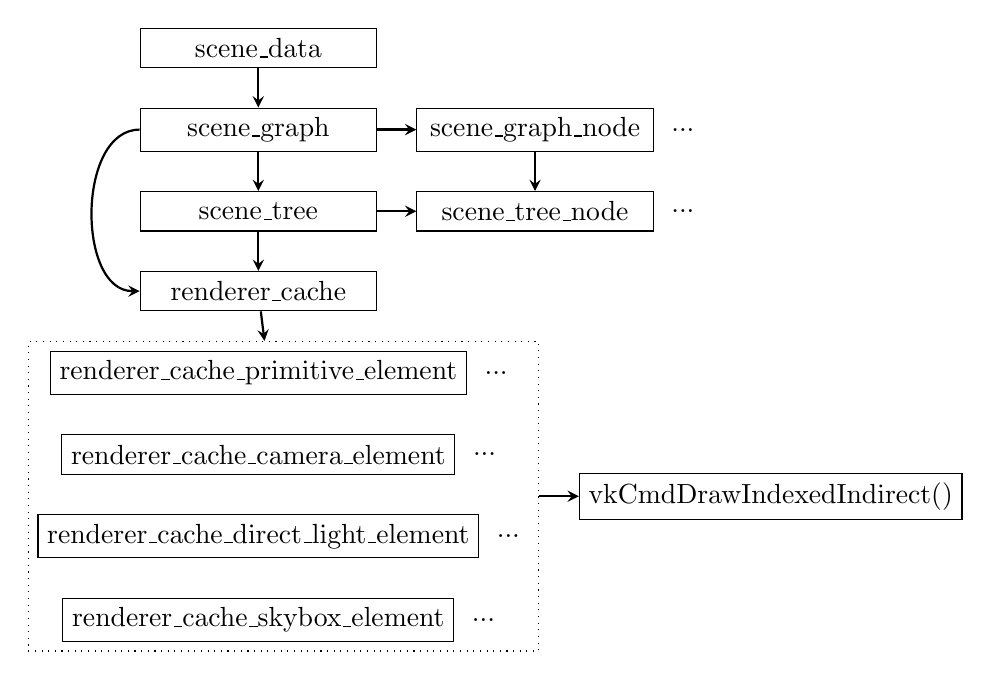
\begin{tikzpicture}[node distance=0.5cm]
		\tikzstyle{entity} = [rectangle, minimum width=3cm, minimum height=0.5cm,text centered, draw=black]
		\tikzstyle{flows} = [thick,->,>=stealth]
		
		\node (scene_data) [entity] {scene\_data};
		\node (scene_graph) [entity, below = of scene_data] {scene\_graph};
		\node (scene_tree) [entity, below = of scene_graph] {scene\_tree};
		\node (renderer_cache) [entity, below = of scene_tree] {renderer\_cache};
		
		\node (scene_graph_node) [entity, right = of scene_graph] {scene\_graph\_node};
		\node (scene_graph_node_dots) [right = 1mm of scene_graph_node] {...};
		\node (scene_tree_node) [entity, right = of scene_tree] {scene\_tree\_node};
		\node (scene_tree_node_dots) [right = 1mm of scene_tree_node] {...};
		
		\node (renderer_cache_primitive_element) [entity, below = of renderer_cache] {renderer\_cache\_primitive\_element};
		\node (renderer_cache_primitive_element_dots) [right = 1mm of renderer_cache_primitive_element] {...};
		\node (renderer_cache_camera_element) [entity, below = of renderer_cache_primitive_element] {renderer\_cache\_camera\_element};
		\node (renderer_cache_camera_element_dots) [right = 1mm of renderer_cache_camera_element] {...};
		\node (renderer_cache_direct_light_element) [entity, below = of renderer_cache_camera_element] {renderer\_cache\_direct\_light\_element};
		\node (renderer_cache_direct_light_element_dots) [right = 1mm of renderer_cache_direct_light_element] {...};
		\node (renderer_cache_skybox_element) [entity, below = of renderer_cache_direct_light_element] {renderer\_cache\_skybox\_element};
		\node (renderer_cache_skybox_element_dots) [right = 1mm of renderer_cache_skybox_element] {...};
		\node(renderer_cache_elements)[draw,dotted,fit=(renderer_cache_primitive_element) (renderer_cache_camera_element) (renderer_cache_direct_light_element) (renderer_cache_skybox_element) (renderer_cache_direct_light_element_dots)] {};
		
		\node (vkCmdDrawIndexedIndirect) [entity, right = of renderer_cache_elements] {vkCmdDrawIndexedIndirect()};
		
		\draw [flows] (scene_data) edge[out=-90,in=90] (scene_graph);
		\draw [flows] (scene_graph) edge[out=180,in=180] (renderer_cache);
		\draw [flows] (scene_graph) edge[out=-90,in=90] (scene_tree);
		\draw [flows] (scene_graph) edge[] (scene_graph_node);
		\draw [flows] (scene_graph_node) edge[] (scene_tree_node);
		\draw [flows] (scene_tree) edge[out=-90,in=90] (renderer_cache);
		\draw [flows] (scene_tree) edge[] (scene_tree_node);
		\draw [flows] (renderer_cache) edge[] (renderer_cache_elements);
		\draw [flows] (renderer_cache_elements) edge[] (vkCmdDrawIndexedIndirect);
		
	\end{tikzpicture}
	\caption{Obiekty biorące udział w procesie konwersji sceny (opracowanie własne)}
	\label{scene_process}
\end{figure}

\subsubsection{Dane sceny scene\_data}
Obiekt \textit{scene\_data} reprezentuje dane sceny wczytane z bazy zasobów. Jest one używany przez moduł sceny do konstrukcji grafu sceny \textit{scene\_graph}.

Obiekt utrzymuje listy dwukierunkowe zawierającą wszystkie utworzone obiekty zasobów, w tym ich domyślne warianty.
Przykładowo domyślny obraz \textit{asset\_image} to obraz 2D o rozmiarze 1x1 mający 4 8-bitowe komponenty o wartości 255.

Wśród wszystkich obiektów zasobów składających się na dane sceny dodatkowo wyróżnia się:
\begin{itemize}
	\item węzły główne: używane jako punkty początkowe podczas tworzenia grafu sceny,
	\item używany skybox: może być zmieniony w konfiguracji zasobów,
	\item aktywna czcionka: sterowana konfiguracją globalną,
	\item domyślna kamera: używana w przypadku braku węzła z przypisaną kamerą.
\end{itemize}

Metody \textit{serialize()} i \textit{deserialize()} podobnie jak analogiczne metody obiektów zasobów pozwalają na zapis i odczyt danych sceny do bazy zasobów.

Metoda \textit{create\_with\_gltf\_file()} jest wywoływana wyłącznie przez potok zasobów.
Jej wejściem jest nazwa tworzonej sceny i ścieżka do katalogu zawierającego zasób 3D w formacie \textit{glTF} wraz z konfiguracją zasobów.
Oba zasoby wejściowe są parsowane przy użyciu biblioteki \textit{cgltf} i obiektu \textit{config}.
Wynik parsowania jest używany do stworzenia i wypełnienia danych sceny.
Ta metoda wraz z metodą \textit{serialize()} stanowi główną częścią potoku zasobów - obiekt stworzony na podstawie zasobów wejściowych jest serializowany do zasobu wyjściowego (bazy zasobów).

Metoda \textit{create\_with\_asset\_db()} jest wywoływana w czasie wykonywania i wczytuje dane sceny o żądanej nazwie z bazy zasobów.

\subsubsection{Graf sceny scene\_graph i drzewo sceny scene\_tree}
Obiekty \textit{scene\_graph} i \textit{scene\_tree} reprezentują kolejno graf i drzewo sceny.
Są one tworzone na podstawie danych sceny używając metody \textit{create\_with\_scene\_data()}.

Implementacja została zainspirowana techniką modelowania hierarchicznego opracowaną w firmie Nvidia \cite{ADVANCEDSCENEGRAPH}.
Graf sceny jest konwertowany na formę pośrednią zwaną drzewem sceny w sposób zapewniający unikalną ścieżkę z korzenia drzewa do jego liści.
Uprasza to klasyczny proces konwersji sceny algorytmem \ref{RenderujGrafSceny} - podczas przechodzenia drzewa sceny każdy węzeł może być napotkany tylko raz.
Właściwość ta pozwala na wprowadzenie do węzła stanu nagromadzonego (struktura \textit{scene\_tree\_node\_accumulated}) zawierającego aktualny wynik działania algorytmu.
Konwersja sceny sprowadza się wtedy do całkowitej propagacji stanu nagromadzonego od korzenia do liści, w których jest on całkowicie wypełniony i tym samym zawiera wszystkie informacje wymagane do wyemitowania polecenia rysowania.

Diagramy \ref{triangles_scene_graph} i \ref{triangles_scene_tree} przedstawiają wygenerowane metodami \textit{debug\_print()} graf i drzewo sceny składającej się z dwóch trójkątów używających tej samej siatki, ale różniących się pozycją.
\begin{figure}[htbp]
	\centering
	\includegraphics[width=0.6\textwidth]{images/scene_graph.png}
	\caption{Przykładowy graf sceny zawierającej dwa trójkąty (opracowanie własne)}
	\label{triangles_scene_graph}
\end{figure}
Graf sceny składa się z czterech węzłów \textit{scene\_graph\_node}: korzenia oraz dwóch węzłów utworzonych na podstawie zasobów obiektów wskazujących na ten sam węzeł z zasobem prymitywu.
Węzły grafu sceny obserwują utworzone na ich podstawie podczas procesu konwersji węzły drzewa sceny, co pozwala na aktualizację i propagację ich stanu nagromadzonego po zmianach w węźle grafu sceny bez konieczności całkowitego odtworzenia drzewa sceny.
\begin{figure}[htbp]
	\centering
	\includegraphics[width=1.0\textwidth]{images/scene_tree.png}
	\caption{Przykładowe drzewo sceny zawierającej dwa trójkąty (opracowanie własne)}
	\label{triangles_scene_tree}
\end{figure}
Drzewo sceny składa się z pięciu węzłów \textit{scene\_tree\_node} posiadających stan nagromadzony:
\begin{itemize}
	\item korzeń: stan posiada lokalnym przekształceniem będącym macierz obrotu zmieniająca prawoskrętną przestrzeń modelu glTF na lewoskrętną przestrzeń używaną przez silnik;
	\item dwa węzły utworzone na podstawie węzłów z zasobami obiektów: stan posiada lokalne przekształcenie zmieniające pozycję trójkątów;
	\item dwa liście utworzone na podstawie węzłów z zasobami prymitywu: stan posiada wskaźnik do zasobu prymitywu.
\end{itemize}
Po zakończeniu propagacji stanu nagromadzonego liście posiadają informacje o prymitywie i jego globalnym przekształceniu.
Liście drzewa sceny są dodawane do pamięci podręcznej renderera.


\subsection{Renderer}

Główny moduł silnika odpowiedzialny za właściwy proces renderowania.
Moduł renderera jest używany do zaimplementowania aplikacji renderującej przykładową scenę.


\subsubsection{Renderer}
Obiekt \textit{renderer} to główny obiekt modułu odpowiedzialny za integrację wszystkich obiektów silnika w celu rozpoczęcia pętli głównej programu i wyrenderowanie sceny.
Obiekt tworzy i używa następujące obiekty:
\begin{itemize}
	\item konfiguracja globalna \textit{data\_config},
	\item baza zasobów \textit{asset\_db},
	\item dane sceny \textit{scene\_data},
	\item graf sceny \textit{scene\_graph},
	\item pamięć podręczna renderowania \textit{renderer\_cache},
	\item urządzenie \textit{device},
	\item łańcuch wymiany \textit{swap\_chain},
	\item stan renderera \textit{render\_state},
	\item graf renderowania \textit{render\_graph}.
\end{itemize}

Po stworzeniu obiektu aplikacja musi skonstruować i skompilować początkowo pusty graf renderowania.
Następnie może ona rozpocząć pętlę główną programu metodą \textit{run\_main\_loop()}, która renderuje pojedyncza klatkę w locie używając następujących kroków:
\begin{itemize}
	\item zaktualizuj stan renderera wejściową funkcją zwrotną \textit{updateFunc};
	\item czekaj aż ogrodzenie \textit{inFlightFences} obecnej klatki w locie zasygnalizuje zakończenie wykonywania poprzednio nagranego bufora poleceń i gotowość do ponownego nagrywania;
	\item pobierz prezentowalny obraz funkcją \textit{vkAcquireNextImageKHR()};
	\item odtwórz łańcuch wymiany jeśli jest nieaktualny i pomiń resztę iteracji pętli;
	\item zaktualizuj i skopiuj do GPU stan renderera i graf renderowania używając ich metod \textit{update()} i \textit{send\_to\_device()};
	\item zresetuj bufor poleceń i rozpocznij nagrywanie;
	\item dowiąż stan renderera (jednolite bufory, zbiór deskryptorów i stałe push);
	\item nagraj przebiegi renderowania używając grafu renderowania;
	\item zakończ nagrywania;
	\item wyślij bufor poleceń do kolejki graficznej funkcją \textit{vkQueueSubmit()} zapewniając synchronizację poprzez oczekiwanie na semafor \textit{imageAvailableSemaphores} oraz sygnalizację semafor \textit{renderFinishedSemaphores} i zresetowanego ogrodzenia \textit{inFlightFences};
	\item prezentuj wynik renderowania funkcją \textit{vkQueuePresentKHR()} zapewniając synchronizację poprzez oczekiwanie na semafor \textit{renderFinishedSemaphores}
	\item odtwórz łańcuch wymiany jeśli jest nieaktualny;
	\item przejdź do kolejnej klatki w locie (metoda \textit{advance\_to\_next\_frame()} obiektu \textit{sync}).
\end{itemize}

W dalszych sekcjach przybliżono obiekty renderera i używającą go przykładową aplikację.


\subsubsection{Pamięć podręczna renderera renderer\_cache}
Pamięć podręczna renderera \textit{renderer\_cache} jest niskopoziomową reprezentacją sceny pośredniczącą pomiędzy modułami sceny i renderera.
Obiekt jest podstawowym źródłem informacji o scenie używanym przez resztę obiektów modułu.

Inicjalizację pamięci podręcznej renderera można podzielić na dwie fazy - graf sceny wypełniania obiekt informacjami o scenie, który jest następnie używany do wypełnienia obiektów używanych przez renderer:
\begin{itemize}
	\item stan renderera,
	\item stany przebiegów renderowania,
	\item grup poleceniami rysowania.
\end{itemize}

Obiekt jest złożony z list elementów \textit{renderer\_cache\_*\_element}:
\begin{itemize}
	\item \textit{renderer\_cache\_primitive\_element}: element prymitywu;
	\item \textit{renderer\_cache\_camera\_element}: element kamery;
	\item \textit{renderer\_direct\_light\_element}: element światła bezpośrednie;
	\item \textit{renderer\_skybox\_element}: element skybox;
	\item \textit{renderer\_font\_element}: element czcionki.
\end{itemize}
Elementy są dodawane przez graf sceny używając metod \textit{add\_*\_element()}.

Obiekt jest używany do aktualizacji stanu renderera:
\begin{itemize}
	\item Metoda \textit{update\_geometry()} dodaje geometrię prymitywów do jednolitego bufora geometrii.
	\item Metoda \textit{update\_textures()} dodaje tekstury używane przez elementy do tekstur \textit{textures}.
\end{itemize}

\item Metoda \textit{add\_new\_primitive\_elements\_to\_batches()} dodaje polecenia rysowania prymitywów do grup poleceniami rysowania.

Aktualizacja stanu renderera i grup poleceń rysowania przy użyciu powyższych metod jest odzwierciedlana aktualizacją stanu elementu.
Przykładowo wywołanie metody \textit{update\_geometry()} aktualizuje strukturę \textit{vertex\_stream\_element} elementów prymitywów offsetami buforów strumienia wierzchołków.
Podobnie metoda \textit{update\_textures()} dodaje tekstury elementu skybox, których identyfikatory są zapamiętywane w elementach.

Zachowanie to pozwala stanom przebiegów renderowania na aktualizację jednolitego bufora stałych informacjami o scenie.
Przykładowo element skybox jest używany do aktualizacji zmiennej \textit{skyboxCubemapTextureId} używanej przez shadery renderujące skybox.


\subsubsection{Grupy poleceń rysowania batches}
Grupa poleceń rysowania \textit{batches} reprezentuje jedno optymalizowane polecenia rysowania utworzone na podstawie elementów prymitywów dodanych metodą \textit{add\_primitive\_element()}.

Metoda \textit{update()} sortuje i konsoliduje dodane elementy prymitywów tworząc tablicę pojedynczych grup poleceń rysowania \textit{batch}.
Pojedyncza grupa poleceń \textit{batch} zawiera wszystkie informacje wymagane do nagrania pojedynczego polecenia rysowania \textit{vkCmdDrawIndexed()} rysującego $n$ kopii mających tą samą geometrię, ale różniących się materiałem i macierzą modelu.

Metoda \textit{record\_draw\_command()} nagrywa do wejściowego bufora poleceń pojedyncze polecenie wielokrotnego rysowania pośredniego \textit{vkCmdDrawIndexedIndirect}, której bufora parametrów jest wypełniany wcześniej stworzoną tablicą obiektów \textit{batch}.
Bufor parametrów jest przekazywany do metody strukturą \textit{batches\_buffer}, która jest zarządzana przez stan przebiegów renderowania.


\subsubsection{Stan renderera renderer\_state i stan przebiegów renderowania render\_pass\_state}
Stan renderera \textit{renderer\_state} zawiera wszystkie obiekty renderera, które są niezależne od stanu przebiegów renderowania.
Są to:
\begin{itemize}
	\item strumień wierzchołków \textit{vertex\_stream},
	\item jednolity bufor geometrii \textit{unified\_geometry\_buffer} (dane globalne współdzielone przez klatki w locie),
	\item tekstury \textit{textures},
	\item jednolity bufor stałych \textit{unified\_constant\_buffer},
	\item deskryptory \textit{descriptors},
	\item synchronizacja \textit{sync}.
\end{itemize}

Podział ten jest spowodowany obsługą odtwarzania łańcucha wymiany - większość stanu przebiegów renderowania, w przeciwieństwie od stanu renderera, zależy od wielkości łańcucha wymiany i dlatego musi być niszczony i ponownie tworzony przez renderer wraz z łańcuchem wymiany.

Metody \textit{update()} i \textit{send\_to\_device()} wywołuje analogiczne metody obiektów renderera.

Stan przebiegów renderowania \textit{render\_pass\_state} jest obiektem analogicznym do stanu renderera i odpowiada za aktualizację jednolitego bufora stałych (dane instancji oraz dane globalne zależne od obecnej klatki w locie) oraz zarządzanie buforami parametrów poleceń rysowania pośredniego.


\subsubsection{Graf renderowania render\_graph}
Graf renderowania \textit{render\_graph} opisuje proces renderowania klatki w formie przebiegów renderowania i używanych przez nie obrazów.
Obiekt jest też odpowiedzialny za zarządzanie wszystkimi przebiegami renderowania \textit{render\_pass} i współdzielonym przez nie stanem przebiegów renderowania \textit{render\_pass\_state}.

Metoda \textit{add\_image\_resource()} jest używana przez aplikację do dodania wszystkich obrazów, które będą używane przez przebiegi renderowania. Wyjątkiem są prezentowalne obrazy, które są dodawane automatycznie.

Dodane obrazy są przechowywane w liście struktur \textit{render\_graph\_resource} posiadającej:
\begin{itemize}
	\item nazwę zasobu;
	\item typ obrazu;
	\item identyfikator tekstury pozaekranowej: obsługa klatek w locie wymaga wewnętrznej duplikacji używanych tekstury pozaekranowych, dlatego indeks obrazu należącego do obecnej klatki jest przekazywany w jednolitym buforze stałych do shaderów chcących je próbkować;
	\item harmonogram użycia \textit{image\_render\_pass\_usage\_timeline}
\end{itemize}

Harmonogram użycia obrazu \textit{image\_render\_pass\_usage\_timeline} opisuje sposób użycia (odczyt, zapis, odczyt i zapis), format i wartość czyszczenia obrazu na wskroś przebiegów renderowania.
Jest on wypełniony podczas kompilacji i używany do nagrania wymaganych przejść układów obrazów pomiędzy przebiegami renderowania.

Listing \ref{render_graph_images} przedstawia kod przykładowej aplikacji dodający obrazy (G-bufor, bufor głębi i bufor okluzji otoczenia) do grafu renderowania.
\lstset{language=C}
\begin{lstlisting}[caption={Dodawanie obrazów do grafu renderowania przykładowej aplikacji},captionpos=b,label={render_graph_images}]
render_graph_add_image_resource(renderer->renderGraph, "depthBuffer",
image_type_offscreen_depth_buffer);
render_graph_add_image_resource(renderer->renderGraph, "gBuffer0", image_type_offscreen_f16);
render_graph_add_image_resource(renderer->renderGraph, "gBuffer1", image_type_offscreen_f16);
render_graph_add_image_resource(renderer->renderGraph, "gBuffer2", image_type_offscreen_f16);
render_graph_add_image_resource(renderer->renderGraph, "aoBuffer", image_type_offscreen_r8);
\end{lstlisting}

Metoda \textit{add\_render\_pass()} jest używana przez aplikację do dodawania następujących po sobie przebiegów renderowania opisywanych strukturą \textit{render\_pass\_desc}.

Dodane przebiegi renderowania są przechowywane jako węzły grafu renderowania \textit{render\_graph\_render\_pass\_element} posiadające:
\begin{itemize}
	\item przebieg renderowania \textit{render\_pass};
	\item wskaźniki do zasobów \textit{render\_graph\_resource}, które będą używane przez przebieg renderowania:
	\begin{itemize}
		\item prezentowalny obraz: dołączenie koloru);
		\item tekstury pozaekranowe: dołączenia koloru lub próbkowany przez shader);
		\item bufor głębi: dołączenie głębi/szablonu używane do testów głębi z możliwością aktualizacji lub próbkowany przez shader;
	\end{itemize}
	\item stan kompilacji: struktura \textit{rendering\_info} używana nagrania przejść układów powyższych obrazów i rozpoczęcia przebiegu renderowania poleceniem \textit{vkCmdBeginRenderingKHR()}.
\end{itemize}
Wszystkie powyższe obiekty są tworzone na podstawie opisu przebiegu renderowania \textit{render\_pass\_desc}. Listing \ref{render_graph_deferred_geometry} przedstawia kod przykładowej aplikacji dodający przebieg geometrii, który:
\begin{itemize}
	\item używa shadera wierzchołków \textit{deferred\_geometry\_vertex.glsl};
	\item używa shadera fragmentów \textit{deferred\_geometry\_fragment.glsl};
	\item nie renderuje do prezentowalnego obrazu;
	\item używa trzech obrazów G-bufora, które są czyszczone wartością $0,0,0,1$ jeśli są używane po raz pierwszy oraz używane jako dowiązania kolorów;
	\item używa bufora głębi jako dołączenia głębi/szablonu, czyszczonego wartością $0,0$, używanego do testów głębi z operatorem porównania "większy lub równy" i włączonym zapisem;
	\item brak mieszania kolorów;
	\item nagrywa zoptymalizowane polecenie rysowania wszystkich elementów prymitywów podręcznej pamięci renderera.
\end{itemize}
\lstset{language=C}
\begin{lstlisting}[caption={Dodawanie przebiegu geometrii do grafu renderowania przykładowej aplikacji},captionpos=b,label={render_graph_deferred_geometry}]

void render_pass_record_primitive_geometry_draws(render_pass *renderPass, render_pass_frame_state *frameState, VkCommandBuffer commandBuffer) {
	batches_record_draw_command(renderPass->renderPassState->sharedState.rendererCacheBatches,
	commandBuffer, &frameState->rendererCacheBatchesData);
}

render_graph_add_render_pass(renderer->renderGraph, (render_pass_desc){
	.vertexShader = "deferred_geometry_vertex.glsl",
	.fragmentShader = "deferred_geometry_fragment.glsl",
	.useOnscreenColorAttachment = false,
	.offscreenColorAttachmentCount = 3,
	.offscreenColorAttachments =
	{
		{.name = "gBuffer0", .clearValue = {{0.0f, 0.0f, 0.0f, 1.0f}}},
		{.name = "gBuffer1", .clearValue = {{0.0f, 0.0f, 0.0f, 1.0f}}},
		{.name = "gBuffer2", .clearValue = {{0.0f, 0.0f, 0.0f, 1.0f}}},
	},
	.offscreenDepthAttachment =
	{
		.name = "depthBuffer",
		.depthWriteEnable = true,
		.depthTestEnable = true,
		.depthTestOp = VK_COMPARE_OP_GREATER_OR_EQUAL,
		.clearValue = {0.0f, 0.0f},
	},
	.colorBlendingType = color_blending_type_none,
	.recordFunc = render_pass_record_primitive_geometry_draws});
\end{lstlisting}

Metoda \textit{compile()} kompiluje graf renderowania.
Dla każdego węzła metoda oblicza harmonogramy użycia dla używanych przez niego obrazów i następnie używa ich do wypełnienia stanu kompilacji celami renderowania z wymaganymi przez nie przejściami układów obrazów.

Metoda \textit{record\_commands()} iteruje po węzłach używając ich stanu kompilacji do nagrania przebiegów renderowania.

Metody \textit{update()} i \textit{send\_to\_device()} aktualizuje i kopiuje do GPU stan przebiegów renderowania.


\subsubsection{Przebieg renderowania render\_pass}
Przebieg renderowania \textit{render\_pass} jest tworzony na podstawie opisu przebiegu renderowania \textit{render\_pass\_desc} i składa się z:
\begin{itemize}
	\item potoku graficznego \textit{VkPipeline},
	\item programu shaderów \textit{render\_pass\_shader\_program};
\end{itemize}

Potok graficzny jest tworzony na podstawie opisu \textit{render\_pass\_desc} oraz stanu renderowania (stan wejścia wierzchołków zależny od \textit{vertex\_stream}).
Moduły shaderów używane przez potok są tworzone przez program shaderów wywołujący generator shaderów \textit{render\_pass\_shader\_generator}.

Metoda \textit{record()} nagrywa dynamiczny przebieg renderowania z dowiązanym potokiem graficznym i poleceniami rysowania zdefiniowanymi polem \textit{recordFunc} opisu \textit{render\_pass\_desc}.


\subsubsection{Generator shaderów render\_pass\_shader\_generator}
Generator shaderów \textit{render\_pass\_shader\_generator} generuje kod źródłowy GLSL pojedynczego shadera.

Generacja kodu źródłowego sprowadza się do konkatenacji:
\begin{itemize}
	\item dyrektyw preprocesora deklarujących używane rozszerzenia,
	\item stałych preprocesora opisujących:
	\begin{itemize}
		\item używane atrybuty wierzchołka (\textit{IN\_POSITION}, \textit{IN\_NORMAL} itp.),
		\item typ shadera (\textit{SHADER\_VERTEX}, \textit{SHADER\_FRAGMENT}),
		\item wygenerowane stałe (np. \textit{MAX\_DIRECTIONAL\_LIGHT\_COUNT}),
		\item nazwy używanych tekstur pozaekranowych (np. \textit{OFFSCREEN\_TEXTURE\_gBuffer1}),
	\end{itemize}
	\item kwalifikatorów układów dla stałych push, buforów uniform i tablicy tekstur,
	\item zmiennych wejściowych i wyjściowych,
	\item współdzielonego kodu GLSL wczytanego z pliku tekstowego \textit{common.glsl},
	\item funkcji \textit{main()}:
	\begin{itemize}
		\item zmienne z indeksami tekstur pozaekranowych,
		\item kod GLSL wczytany z pliku tekstowego zdefiniowanego w opisie \textit{render\_pass\_desc}.
	\end{itemize}
\end{itemize}


\subsubsection{Przykładowa scena main}
Plik wykonywalny \textit{main} demonstruje działanie silnika poprzez wyrenderowanie sceny zdefiniowanej w konfiguracji globalnej używając grafu renderowania.

Diagram \ref{render_graph_final} przedstawia używany graf renderowania opisujący cieniowane odroczone zintegrowane z okluzję otoczenia \cite{PureDepthSSAO} i dwoma dodatkowymi efektami post-processingu: skybox i tekst debugujący.
\begin{figure}[H]
	\centering
	\begin{tikzpicture}[node distance=1cm]
		\tikzstyle{pass} = [rectangle, minimum width=3.5cm, minimum height=1cm,text centered, draw=black]
		\tikzstyle{resource} = [rectangle, rounded corners, minimum width=3.5cm, minimum height=1cm, text centered, draw=black]
		\tikzstyle{arrow} = [thick,->,>=stealth]
		\tikzstyle{relation} = [densely dotted,->]
		
		\node (gBuffor2) [resource] {Obraz G-bufor \#2};
		\node (gBuffor1) [resource, above = 6mm of gBuffor2] {Obraz G-bufor \#1};
		\node (gBuffor3) [resource, below = 6mm of gBuffor2] {Obraz G-bufor \#3};
		\node (depthResource) [resource, below = 6mm of gBuffor3] {Bufor głębi};
		\node (aoResource) [resource, below = 6mm of depthResource] {Bufor AO};
		\node (presentableImage) [resource, below = 6mm of aoResource] {Prezentowalny obraz};
		
		\node (geometryPass) [pass, right = 3cm of gBuffor1] {Przebieg geometrii};
		\node (aoPass) [pass, below = of geometryPass] {Okluzja otoczenia};		
		\node (lightingPass) [pass, below = of aoPass] {Przebieg oświetlenia};
		\node (skyboxPass) [pass, below = of lightingPass] {Skybox};
		\node (debugTextPass) [pass, below = of skyboxPass] {Tekst debugowania};
		
		\draw [relation] (geometryPass) edge (aoPass);
		\draw [relation] (aoPass) edge (lightingPass);
		\draw [relation] (lightingPass) edge (skyboxPass);
		\draw [relation] (skyboxPass) edge (debugTextPass);
		
		\draw [arrow] (geometryPass) edge[out=180-10,in=0,looseness=0] (gBuffor1);
		\draw [arrow] (geometryPass) edge[out=180-5,in=0,looseness=0] (gBuffor2);
		\draw [arrow] (geometryPass) edge[out=180+0,in=0+5,looseness=0] (gBuffor3);
		\draw [arrow] (geometryPass) edge[out=180+5,in=0+10,looseness=0] (depthResource);
		
		\draw [arrow] (gBuffor1) 		edge[out=0-5,in=180-10,looseness=0] (aoPass);
		\draw [arrow] (gBuffor3) 		edge[out=0,in=180-5,looseness=0] (aoPass);
		\draw [arrow] (depthResource) 	edge[out=0+5,in=180+0,looseness=0] (aoPass);
		\draw [arrow] (aoPass) 			edge[out=180+5,in=0+5,looseness=0] (aoResource);
		
		\draw [arrow] (gBuffor1) edge[out=0-10,in=180-10,looseness=0] (lightingPass);
		\draw [arrow] (gBuffor2) edge[out=0,in=180-5,looseness=0] (lightingPass);
		\draw [arrow] (gBuffor3) edge[out=0-5,in=180+0,looseness=0] (lightingPass);
		\draw [arrow] (depthResource) edge[out=0,in=180+5,looseness=0] (lightingPass);
		\draw [arrow] (aoResource) edge[out=0,in=180+10,looseness=0] (lightingPass);
		\draw [arrow] (lightingPass) edge[out=180+15,in=0+10,looseness=0] (presentableImage);
		
		\draw [arrow] (depthResource) edge[out=0-5,in=180-5,looseness=0] (skyboxPass);
		\draw [arrow] (presentableImage) edge[out=0+5,in=180+0,looseness=0] (skyboxPass);
		\draw [arrow] (skyboxPass) edge[out=180+5,in=0,looseness=0] (presentableImage);
		
		\draw [arrow] (presentableImage) edge[out=0-5,in=180-5,looseness=0] (debugTextPass);
		\draw [arrow] (debugTextPass) edge[out=180+5,in=0-10,looseness=0] (presentableImage);
		
	\end{tikzpicture}
	\caption{Graf renderowania przykładowej sceny (opracowanie własne)}
	\label{render_graph_final}
\end{figure}

Listing \ref{main_final} przedstawia kod funkcji \textit{main()} przykładowej aplikacji uruchamiający renderer.
\lstset{language=C}
\begin{lstlisting}[caption={Uruchomienie renderera w funkcji \textit{main()} przykładowej aplikacji},captionpos=b,label={main_final}]
void render_pass_record_draws(render_pass *renderPass, render_pass_frame_state *frameState, VkCommandBuffer commandBuffer) {
	batches_record_draw_command(renderPass->renderPassState->sharedState.rendererCacheBatches, commandBuffer, &frameState->rendererCacheBatchesData);
}

void update_func(renderer *renderer, double fps, double dt) {
	device *vkd = renderer->vkd;
	render_state *renderState = renderer->renderState;
	if (renderState->config->global.controlsEnabled == 1) { ... }
}

int main(int argc, char *argv[]) {
	platform_create(argc, argv);
	renderer *renderer = renderer_create();
	
	render_graph_add_image_resource(renderer->renderGraph, "gBuffer0", image_type_offscreen_f16);
	...
	render_graph_add_render_pass(
		renderer->renderGraph,
		(render_pass_desc){
			...
			.recordFunc = render_pass_record_primitive_geometry_draws
		}
	);
	...
	
	renderer_run_main_loop(renderer, update_func);
	
	renderer_destroy(renderer);
	platform_destroy();
	return 0;
}
\end{lstlisting}


\chapter{Badania}
\label{chap:research}

Ten rozdział zawiera zrzuty ekranu pokazujące wyrenderowane przykładowe sceny.
// HIRO więcej opis

\section{Przykładowe sceny}

Używane sceny zostały przygotowane na podstawie zebranych przez Khronos w repozytorium \cite{GLTFSAMPLEMODELS} następujących przykładowych modelów glTF przedstawiających:
\begin{itemize}
	\item \textit{MetalRoughSpheres}: różne wartości metalu i chropowatości materiałów używając sfer, patrz rys. \ref{screenshot_metalroughspheres};
	\item \textit{DamagedHelmet}: uszkodzony w walce hełm sci-fi, patrz rys. \ref{screenshot_damagedhelmet};
	\item \textit{Sponza}: wnętrze budynku inspirowane pałacem Sponza, często używane do testowania oświetlenia, patrz rys. \ref{screenshot_sponza}.
\end{itemize}

\begin{figure}[!htb]
	\centering
	\includegraphics[width=0.8\textwidth]{images/render_metalroughspheres.png}
	\caption{Wynik renderowania sceny MetalRoughSpheres (opracowanie własne)}
	\label{screenshot_metalroughspheres}
\end{figure}

\begin{figure}[!htb]
	\centering
	\includegraphics[width=0.8\textwidth]{images/render_damagedhelmet.png}
	\caption{Wynik renderowania sceny DamagedHelmet (opracowanie własne)}
	\label{screenshot_damagedhelmet}
\end{figure}

\begin{figure}[!htb]
	\centering
	\includegraphics[width=0.8\textwidth]{images/render_sponza.png}
	\caption{Wynik renderowania sceny Sponza (opracowanie własne)}
	\label{screenshot_sponza}
\end{figure}

\section{Przykładowe sceny}

// TODO: Prezentacja renderdoc
// TODO: Profiling różne sceny.
// TODO: test: technika filtrowanie anizotropowe, usuń TRANSIENT
// TODO: test: usuń mipmapy, usuń multidraw

\chapter{Podsumowanie}
\label{chap:summary}

// TODO

// TODO streaming
// TODO tekstury emissive
\include{chapters/7_wykazy}
\end{document}
